% Official template for
% https://topology.journals.yorku.ca/index.php/tp/about/submissions
% Version 2025-04-25


\documentclass{amsart}
\usepackage{proc}
\usepackage{hyperref}
\usepackage{wrapfig, subcaption}
\usepackage{amsmath, amsthm, amssymb, physics, bbm}
\usepackage{enumitem}

\DeclareMathOperator{\itr}{int}
\DeclareMathOperator{\id}{id}
\DeclareMathOperator{\Homeo}{Homeo}
\DeclareMathOperator{\mcg}{MCG}

\newtheorem*{formal}{Formal}
\newtheorem*{informal}{Informal}
\newtheorem*{comment}{Author comment}


%    Author info
%%%%%%%%%%%%%%%%%%%%%%%%%%%%%%%%%%%%%%%%%%%%%%%%%%%
%    First author:
\author{Olivia Hu}
\address{Department of Mathematics \& Statistics; Boston University;
Boston, Massachusetts 02215}
%    Current address (if needed):
%\curraddr{}
\email{rayh@bu.edu}
\thanks{This was largely inspired by an REU project under Beth Branman and Mark
Pengitore at UVa, organized by Thomas Koberda.}


%    Second author (if needed):
%\author{Author Two}
%\address{}
%\email{}
%\thanks{Support information for the second author.}
%%%%%%%%%%%%%%%%%%%%%%%%%%%%%%%%%%%%%%%%%%%%%%%%%%%




%    Title
%%%%%%%%%%%%%%%%%%%%%%%%%%%%%%%%%%%%%%%%%%%%%%%%%%%
\title[The Braid Symmetries of a Disk]%
{Boston University Society of Mathematics Colloquium Proceedings \\The Braid Symmetries of a Disk}
%%%%%%%%%%%%%%%%%%%%%%%%%%%%%%%%%%%%%%%%%%%%%%%%%%%




%    General info
%%%%%%%%%%%%%%%%%%%%%%%%%%%%%%%%%%%%%%%%%%%%%%%%%%%
%         https://mathscinet.ams.org/mathscinet/msc/msc2020.html
%         https://zbmath.org/classification/
\keywords{Mapping Class Groups, Geometric Group Theory, Group Theory, Algebraic
Topology, Homotopy, Introduction}
%%%%%%%%%%%%%%%%%%%%%%%%%%%%%%%%%%%%%%%%%%%%%%%%%%%




\begin{document}






\begin{abstract}
	A braid in math is not too far from how it sounds --- a
	collection of strands interlacing and intertwining as they travel through
	paths in space. These braids are interesting creatures.
	Some braids look complex, but are just one twist from being untied; other
	braids can look simple, but are in truth much more obstinate.
	However, the study takes an unexpected turn upon discovering braids, like
	numbers, can be multiplied and divided to create new braids: they
	form an abstract structure called a group. By studying this group, we will
	realize that by studying braids, we are actually also studying the
	symmetries of a disk.
\end{abstract}


\maketitle




\section{Preliminaries and Notation}
In this paper, we will assume a working knowledge of basic set theory and the
functions between them. The bare minimum assumptions on sets and functions are
listed further below. Additionally, we will assume continuity of multivariable
functions --- an understanding on the level of a first multivariate calculus
course should be enough to follow intuitively. Finally, we assume
elementary knowledge of matrices and determinants, though this is purely
contained in examples and informal discussions --- it is not strictly necessary
to understand the core content.

This is technically all the required prerequisites, but the reader without
any previous exposure to group theory may find this paper unfairly demanding.
Nonetheless, Section \ref{intro-to-groups} gives a primer on all the group
theory required from the beginning. We hope it is enough to fill in any gaps in
knowledge.

Throughout this paper, many of the definitions and proofs will come
with informal discussions alongside the full technical details. It is not
necessary to fully understand every technical detail, only to glean some
intuition. The formal proofs are generally not essential for the story, so feel
free to skip them. The
subject of this paper is
very visual, and the core ideas can nearly always be grasped by intuition alone.

Readers are encouraged to skip any sections they are already familiar with.

\subsection*{Notation}
\begin{tabular}{c l}
	\(\varnothing\) & The empty set\\
	\(s\in S\) & \(s\) is an element of the set \(S\)\\
	\(A\subset B\) & \(A\) is a subset of \(B\), or \(a\in A\) implies \(a\in B\)\\
	\(A \cup B\) & The union of \(A\) and \(B\) \(\{s : s\in A~\text{or}~s\in
	B\}\)\\
	\(A\cap B\) & The intersection of \(A\) and \(B\) \(\{s: s\in
	A~\text{and}~s\in B\}\)\\
	\(A\setminus B\) & The set difference of \(A\) and \(B\) \(\{s : s\in
	A~\text{and}~s\notin B\}\)\\
	\(A\times B\) & The cartesian product \(\{(a, b) : a\in A ~\text{and}~ b\in
	B\}\)\\
	\(S^n\) & The cartesian product \(\{(s_1,
	s_2, \ldots, s_n) : s_j\in S\}\)\\
	\(f: A\to B\) & A function from the set \(A\) to the set \(B\)\\
	\(a\mapsto b\) & (of a function) maps the element \(a\) to the element
	\(b\)\\
	\(\id: A\to A\) & The identity function that takes each point of \(A\) to
	itself.
\end{tabular}

\subsection*{Sets}
\begin{tabular}{c l}
   \(\mathbb{Z}\) & The set of integers \(\{\ldots, -2, -1, 0, 1, 2, \ldots\}\) \\
   \(\mathbb{R}\) & The set of real numbers \\
	\(D^n\) & The \(n\)-dimensional unit disk \(\left\{(x_1, \ldots,
		x_n)\in\mathbb{R}^n :
	\sum_{i=1}^n x_j^2 \le 1\right\}\)\\
	\(S^n\) & The \(n\)-dimensional unit sphere \(\left\{(x_1, \ldots,
		x_{n+1})\subset\mathbb{R}^{n+1} : \sum_{i=1}^{n+1}x_i^2 = 1)\right\}\).
\end{tabular}

\begin{definition}[Properties of functions]
   A function \(f: A\to B\) between sets is \textbf{injective} if for all \(a,
	a'\in A\) such that \(a\ne a'\), \(f(a) \ne f(a')\).

	Likewise, \(f\) is
	\textbf{surjective} if for all \(b\in B\), there exists \(a\in A\) such that
	\(f(a) = b\). If \(f\) is both injective and surjective, we say \(f\) is
	\textbf{bijective}.

	If there exists \(g: B\to A\) such that for all \(a\in A\) and \(b\in B\),
	\[
		(f\circ g)(b) = b ~\text{and}~(g\circ f)(a) = a,
	\] 
	we say \(f\) is \textbf{invertible}.
\end{definition}
\begin{theorem}
	Let \(f: A\to B\) be a function between sets. Then \(f\) is bijective if and
	only if \(f\) is invertible.
\end{theorem}

\section{Introduction to Groups}\label{intro-to-groups}
\begin{definition}[Groups, {\cite[p.~16]{df}}]\label{groups}
   \begin{informal}
      We can think of groups as a way to generalize adding and
		multiplying to more abstract settings. For example, in the familiar
		situation of adding integers together, we can think of addition as a
		function whose input is	an ordered pair \((a, b)\) and whose output is
		another integer we call \(a + b\). We call this a \emph{binary
		operation}, and the operation	\(+\) has the following nice properties in
		the integers:

		\begin{enumerate}[label=(\roman*)]
			\item for all \(a, b, c\in\mathbb{Z}\), \((a + b) + c = a +
			(b + c)\),
			\item for all \(a\in \mathbb{Z}\), \(a + 0 = a = 0 + a\),
			\item for all \(a\in\mathbb{Z}\), \(a + (-a) = 0 = (-a) + a\),
			\item for all \(a, b\in\mathbb{Z}\), \(a + b = b + a\).
		\end{enumerate}

		A group generalizes this idea to more abstract sets than the integers
		and more abstract operations than addition. For instance, we will see in
		Example \ref{D3} later that the symmetries
		of a triangle satisfy properties (i), (ii), and (iii). Further
		in the paper, we will see Mapping Class groups (Def. \ref{mcg}) and Braid
		groups
		(Def. \ref{braidgroup}). Any set
		with an operation that satisfies (i), (ii), and (iii), we call a
		\emph{group} under
		that operation. If we further have property (iv), that group is called
		\emph{abelian}.
	\end{informal} 

	\begin{formal}
		A \textbf{group} is a pair \((G, \ast)\) where \(G\) is a set and
		\(\ast\) is a \textbf{binary operation} 
		\[
		   \ast: G\times G\to G,
		\]
		where we denote \(\ast(g_1, g_2) = g_1\ast g_2\), satisfying the
		\textbf{group axioms}:
		\begin{enumerate}[label=(\roman*)]
			\item \textbf{Associativity}. For all \(g_1, g_2, g_3\in G\), \((g_1\ast
			g_2)\ast g_3 = g_1\ast(g_2\ast g_3)\).
			\item \textbf{Identity}. There exists \(e\in G\) such for all \(g\in G\),
			\(e\ast g = g = g\ast e\). We call \(e\) an \textbf{identity element}
			of \(G\), or simply an identity.
			\item \textbf{Inverses}. For all \(g\in G\), there exists \(h\in G\)
			such that
			\(h\ast g = e = g\ast h\). We call \(h\) an \textbf{inverse} of \(g\).
		\end{enumerate}
		A group that further satisfies 
		\begin{enumerate}[label=(\roman*)]
			\item[(iv)] \textbf{Commutativity}. For all \(g, h\in G\), \(g\ast h =
			h\ast g\)
		\end{enumerate} is called \textbf{abelian}.	
	\end{formal}
\end{definition}

\begin{proposition}[{\cite[p.~18]{df}}]\label{uniqueness}
   If \((G, \ast)\) is a group, then 
	\begin{enumerate}[label=(\roman*)]
		\item The identity of \(G\) is unique,
		\item For each \(g\in G\), the inverse of \(g\) is uniquely determined.
   \end{enumerate}
\end{proposition}
By Proposition \ref{uniqueness}, we can unambiguously denote the identity of a
group \((G, \ast)\) by \(1\) and the inverse of
an element \(g\in G\) by \(g^{-1}\). Then for any \(n\in\mathbb{Z}\) and \(g\in
G\), we define 
\[
   g^n = 
	\begin{cases}
		g^n = 1 & \text{if }n = 0,\\
		\underbrace{g\ast g\ast\cdots\ast g}_{n~\text{times}} &\text{if }n >0,\\
		(g^{-1})^{-n} & \text{if }n<0.
   \end{cases}
\]
If \((G, \ast)\) is abelian, we often
choose the symbols \(0\), \(-g\) and \(ng\) in place of \(1\), \(g^{-1}\), and
\(g^n\). Moving forward, we will refer to a group \((G, \ast)\) simply as \(G\)
if the operation is clear.

\begin{example}
	As discussed in the informal section of Definition \ref{groups}, the
	integers under addition form an abelian group. That is, \((\mathbb{Z}, +)\)
	is an abelian group.
\end{example}

\begin{example}\label{trivial-group}
   Any set \(G\) with just one element, \(G = \{e\}\), is a group by the binary
	operation \(e\ast e = e\). Indeed, this operation is associative, \(e\) is
	the identity, and \(e\) is its own inverse. This group is abelian as well.

	We call this the \textbf{trivial group}.
\end{example}

\begin{example}
   The integers under multiplication do not form a group because no elements
	besides \(0\), \(-1\), and \(1\) have multiplicative inverses. That is,
	\((\mathbb{Z}, \cdot)\) is not a group.
\end{example}

\begin{example}\label{Rtimes}
   The real numbers under addition, \((\mathbb{R}, +)\), forms a group for
	similar reasons to \((\mathbb{Z}, +)\). However, the real numbers
	under multiplication, \((\mathbb{R}, \cdot)\), does not form a group because
	\(0\) does not have a multiplicative inverse. However, if we define 
	\[
		\mathbb{R}^\times = \mathbb{R}\setminus\{0\},
	\] 
	then \((\mathbb{R}^\times, \cdot)\) forms an abelian group.
\end{example}

\begin{example}
   The integers under subtraction, \((\mathbb{Z}, -)\), is not a group.
	Although \(-\) admits an identity and inverses, \(-\) is not associative.
	For example,
	\[
		(1 - 2) - (-3) = 2
	\]
	while 
	\[
	   1-(2-(-3)) = -4.
	\]
\end{example}

\begin{example}\label{matrices}
   Fix a positive integer \(n\). The space \(M(n, \mathbb{R})\) of \(n\times
	n\) matrices is not a group under multiplication. Although the
	multiplication is associative and the diagonal matrix of \(1\)'s is an
	identity, not every matrix admits an inverse. For example, 
	\[
	   \begin{bmatrix}
			2 & 6\\
			1 & 3
	   \end{bmatrix}\in M(2, \mathbb{R})
	\]
	has determinant \(0\), thus is not invertible.

	If we restrict to the invertible matrices, \(GL(n, \mathbb{R})\subset M(n,
	\mathbb{R})\), then \(GL(n, \mathbb{R})\) is a group under multiplication.
	Note \((GL(n, \mathbb{R}), \cdot)\) is not abelian. For example, 
	\[
		\begin{bmatrix}
			1 & 1\\
			0 & 1
		\end{bmatrix} 
		\begin{bmatrix}
			1 & 0\\
			1 & 1
		\end{bmatrix}
		= 
		\begin{bmatrix}
			2 & 1\\
			1 & 1
		\end{bmatrix},
	\]
	but 
	\[
	   \begin{bmatrix}
			1 & 0\\
			1 & 1
	   \end{bmatrix}
		\begin{bmatrix}
			1 & 1\\
			0 & 1
		\end{bmatrix}
		= 
		\begin{bmatrix}
			1 & 1\\
			1 & 2
		\end{bmatrix}.
	\]
\end{example}

\begin{example}[Dihedral group]\label{D3}
   Our first unfamiliar example: the symmetries of a triangle, \(D_3\), form a
	group under composition \(\circ\).

	By symmetries of a triangle, we mean this. Given an equilateral triangle,
	counterclockwise rotations by \(0\), \(2\pi/3\), and \(4\pi/3\) about the
	center result in the same triangle with the vertices in different positions.
	We call these rotations \(e\), \(R\), and \(R^2\) respectively. In Figure
	\ref{D3elements}, these rotations correspond to (a), (b), and (c). 

	Another three symmetries are given by reflections across the three altitudes
	of the triangle. We call these reflections \(F_1\), \(F_2\), and \(F_3\),
	pictured in (d), (e), and (f) of Figure \ref{D3elements}. These symmetries
	comprise the elements of \(D_3\), making six in total.

	\begin{figure}[!ht]
		\begin{subfigure}{.5\textwidth}
			\centering
			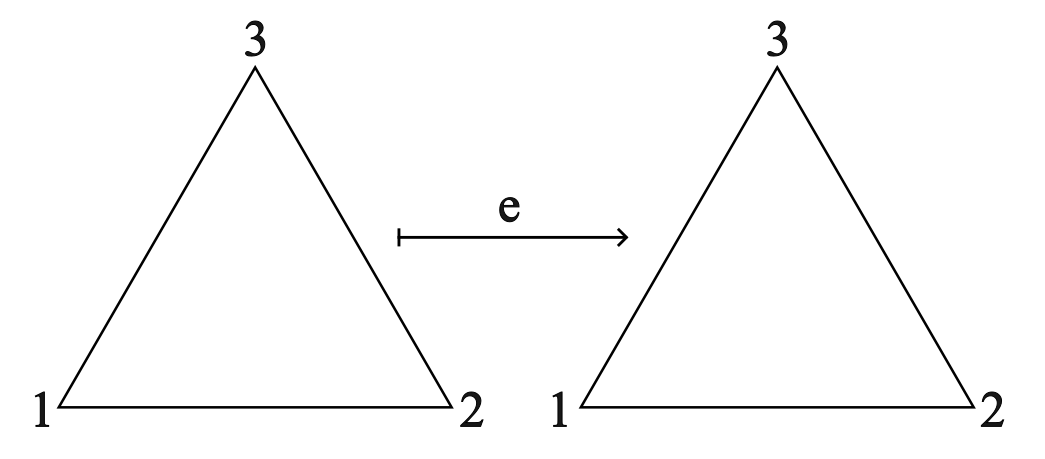
\includegraphics[width=.9\linewidth]{Inkscape Files/D3e.png}
			\caption{Rotation by \(0\).}
		\end{subfigure}%
		\begin{subfigure}{.5\textwidth}
			\centering
			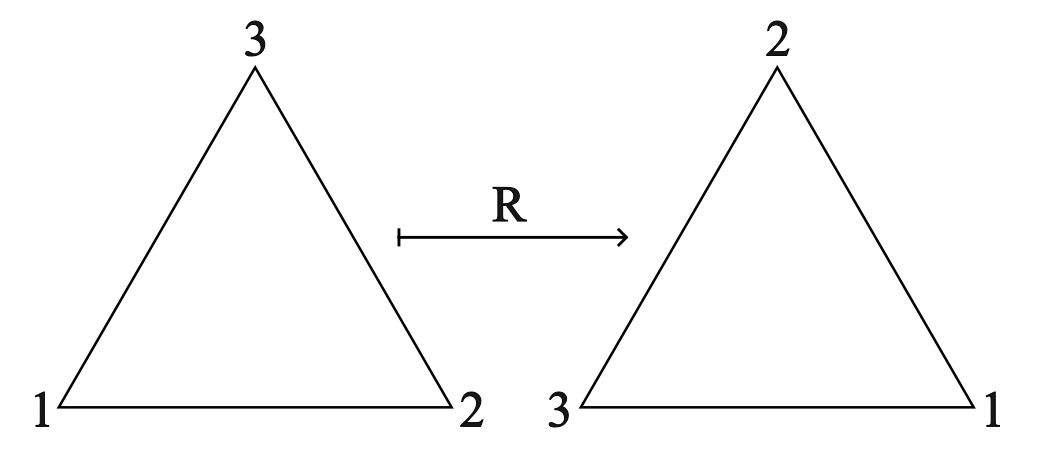
\includegraphics[width=.9\linewidth]{Inkscape Files/D3R1.png}
			\caption{Rotation counterclockwise by \(2\pi/3\)}
		\end{subfigure}%
		\\
		\begin{subfigure}{.5\textwidth}
			\centering
			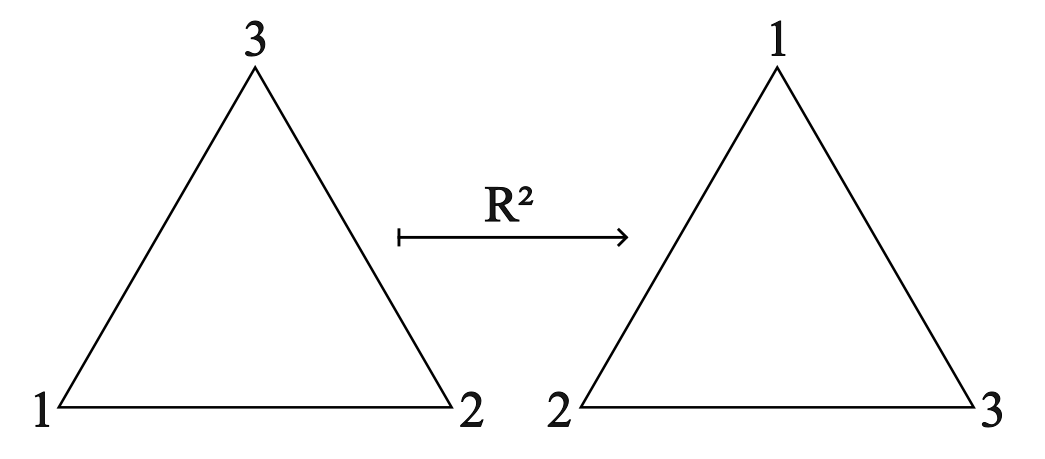
\includegraphics[width=.9\linewidth]{Inkscape Files/D3R2.png}
			\caption{Rotation counterclockwise by \(4\pi/3\).}
		\end{subfigure}%
		\begin{subfigure}{.5\textwidth}
			\centering
			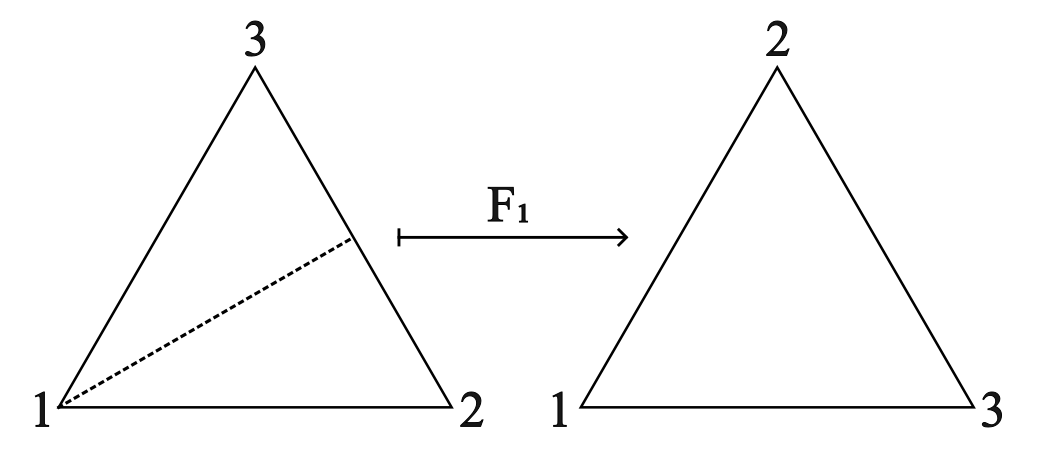
\includegraphics[width=.9\linewidth]{Inkscape Files/D3F1.png}
			\caption{Reflection over altitude from bottom left vertex.}
		\end{subfigure}%
		\\
		\begin{subfigure}{.5\textwidth}
			\centering
			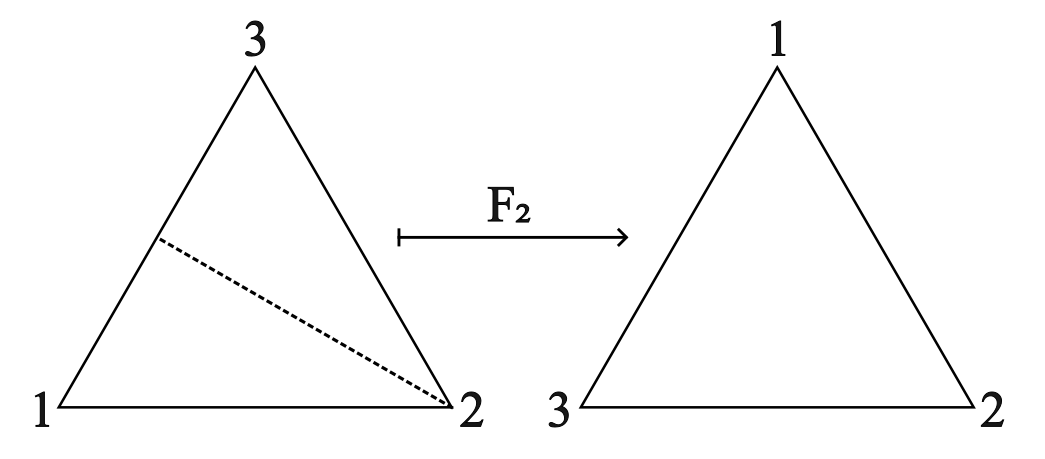
\includegraphics[width=.9\linewidth]{Inkscape Files/D3F2.png}
			\caption{Reflection over altitude from bottom right vertex.}
		\end{subfigure}%
		\begin{subfigure}{.5\textwidth}
			\centering
			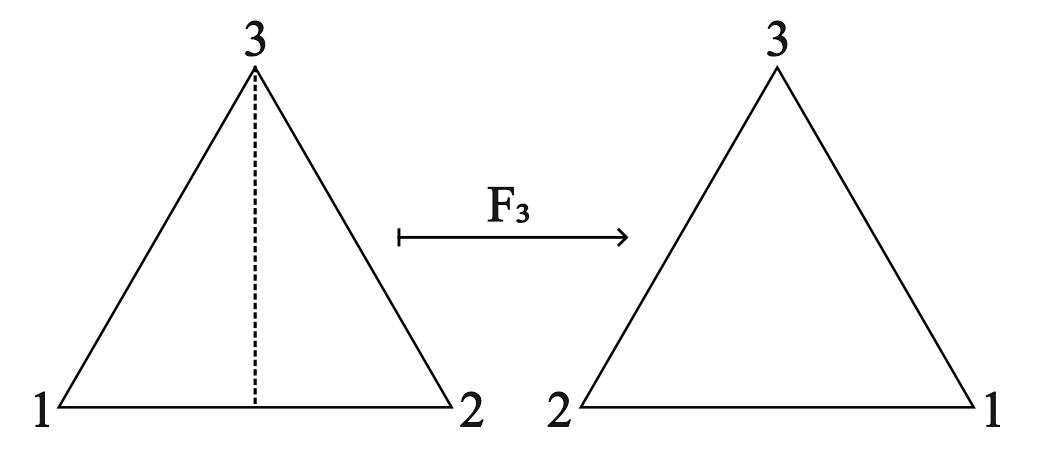
\includegraphics[width=.9\linewidth]{Inkscape Files/D3F3.png}
			\caption{Reflection over altitude from top vertex.}
		\end{subfigure}
		\caption{Symmetries of the triangle.}
		\label{D3elements}
	\end{figure}

	The operation is composition --- that is, if \(A, B\in D_3\), then \(A\circ
	B\) means apply \(B\) to the triangle, then apply \(A\) to the resulting
	triangle (see Examples in Figure	\ref{D3operations}). Note that \(R^2\) is
	simply \(R\circ R\), justifying the notation.
	\begin{figure}[!h]
		\centering
		\begin{subfigure}{.75\textwidth}
			\centering
			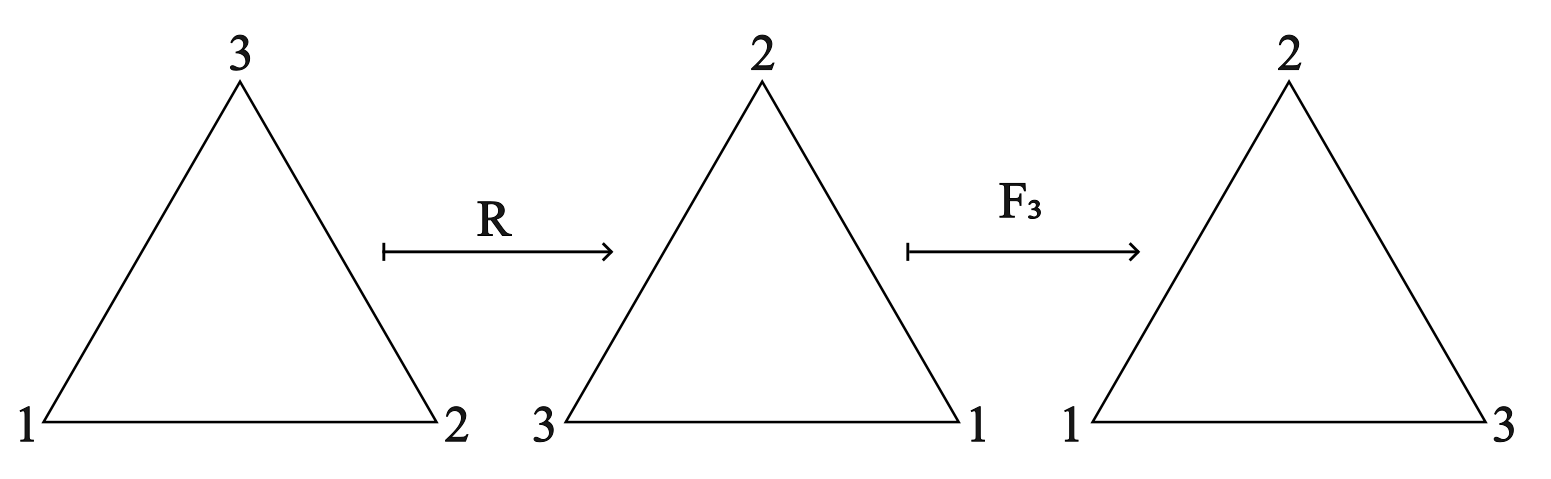
\includegraphics[width=.9\linewidth]{Inkscape Files/D3RF3.png}
			\caption{The composition \(F_3\circ R\). Note this is the same as
			\(F_1\).}
		\end{subfigure}%
		\\
		\begin{subfigure}{.77\textwidth}
			\centering
			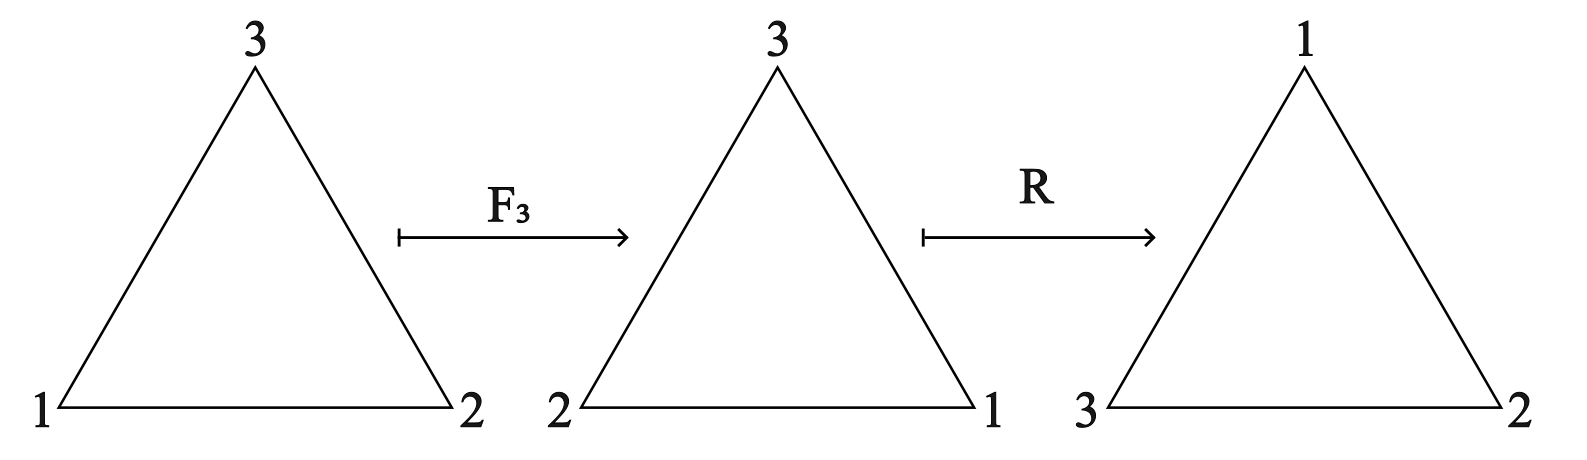
\includegraphics[width=.9\linewidth]{Inkscape Files/D3F3R.png}
			\caption{The composition \(R\circ F_3\). Note this is the same as
			\(F_2\).}
		\end{subfigure}%
		\caption{Examples of compositions in \(D_3\). Observe \(F_3\circ R\ne
		R\circ F_3\).}
		\label{D3operations}
	\end{figure}
	We can work out by force that	for any two elements \(A, B\in D_3\), \(A\circ
	B\in D_3\), so \(\circ\) is a well-defined binary operation \(D_3\times
	D_3\to D_3\).

	In fact, \(\circ\) is associative, \(e\) is the identity, and every element
	has an inverse (\(R^{-1} = R^2\), the remaining elements are their own
	inverses). It follows that	\((D_3, \circ)\) is a group. Note that \(D_3\) is
	not abelian by the Example in Figure \ref{D3operations}.

	In general, the symmetries of an \(n\)-gon is denoted \(D_n\), and \((D_n,
	\circ)\) is a group with \(2n\) elements. This is known as the
	\textbf{Dihedral group}.
\end{example}

\begin{example}[Symmetric group]\label{sym}
   Let \(n\in\mathbb{Z}\) be positive. A \textbf{permutation} on the set \(S =
	\{1, 2, \ldots, n\}\) is a bijection
	\(S\to S\). We denote by \(S_n\) the set of all permutations of \(S\). Note
	that the identity map \(\mathbbm{1}\in S_n\) that sends every element to
	itself is an identity
	under composition. That is, for every \(\sigma\in S_n\), 
	\[
		\sigma\circ\mathbbm{1} = \mathbbm{1}\circ\sigma = \sigma.
	\]
	Moreover, bijections are invertible, so \(\sigma\in S_n\) implies there
	exists \(\sigma^{-1}\in S_n\). Finally, function composition is associative,
	so \((S_n, \circ)\) is a group. We call this the \textbf{symmetric group on
	\(n\) indices}.
\end{example}


\begin{definition}\label{homiso}
	\begin{informal}
		Note that the Dihedral group \(D_3\) of Example \(\ref{D3}\) is kind of
		similar to the symmtric group \(S_3\) of Example \(\ref{sym}\). For example,
		note that the rotation \(R\) by \(2\pi/3\) of Figure \(\ref{D3elements}\)(b)
		maps the indices like
		\[
		   1\mapsto 3, \; 2\mapsto 1,\; 3\mapsto 2.
		\]
		But this is a permutation of \(\{1, 2, 3\}\), we can define a function
		\(D_3\to S_3\) that sends \(R\) to the permutation above and the other
		symmetries to their corresonding permutations. This hints at
		some deep similarity 
		between \(D_3\) and \(S_3\) --- in fact, we say they are
		\emph{isomorphic}, denoted \(D_3\cong S_3\).

		There are also weaker relationships between groups. For example, it is
		true that for any \(A, B\in GL(n, \mathbb{R})\) (see Example
		\ref{matrices}),
		\[
		   \det(AB) = \det(A)\det(B).
		\]
		That is, the determinant turns multiplication in \(GL(n,
		\mathbb{R})\) into multiplication in \(\mathbb{R}^\times\) (see Example
		\ref{Rtimes}).
		So somehow, the determinant is telling us the multiplications
		on \(GL(n, \mathbb{R})\) and \(\mathbb{R}^\times\) induce somewhat similar
		group structures. We say that \(\det\) is a \emph{homomorphism}. An
		isomorphism is a homomorphism that is really nice --- one that is
		invertible.
	\end{informal}

	\begin{formal}
	   Let \((G, \ast)\), \((G', \star)\) be groups. A \textbf{group homomorphism}
		from \(G\) to \(G'\)	is a map
		\[
		   \varphi: G\to G'
		\]
		such that for all \(a, b\in G\), 
		\[
		   \varphi(a\ast b) = \varphi(a)\star \varphi(b).
		\]
		A group homomorphism \(\varphi: G\to G'\) is a \textbf{group isomorphism}
		if \(\varphi\) is invertible. Then we denote \(G\cong G'\).
	\end{formal}
\end{definition}

\begin{example}\label{identity-homomorphism}
   Given any group \((G, \ast)\), the identity map \(\id: G\to G\), defined by
	\[
	   \id(g) = g
	\]
	for all \(g\in G\), is a group homomorphism. To see this, observe that
	for any \(a, b\in G\),
	\[
	   \id(a\ast b) = a\ast b = \id(a)\ast\id(b).
	\]
	In fact, \(\id\) is also its own inverse, thus an isomorphism.

	A concrete example of this is the familiar function \(f:
	\mathbb{R}\to\mathbb{R}\) defined by \(f(x) = x\).
\end{example}

\begin{example}
	Given any groups \((G, \ast)\), \((G', \star)\), where we denote the
	identity of \(G'\) by \(\mathbbm{1}'\), the function \(\varphi:
	G\to G'\) defined by 
	\[
		\varphi(g) = \mathbbm{1}'
	\]
	for all \(g\in G\) is a group homomorphism.
\end{example}

\begin{example}\label{determinant-map}
	As we discussed in Definition \ref{homiso}, the determinant 
	\[
	   \det: GL(n, \mathbb{R})\to \mathbb{R}^\times
	\]
	is a group homomorphism. In fact, one can show \(\det\) is a surjective
	but not injective	homomorphism.
\end{example}

\begin{example}\label{2Z}
	 The function \(\varphi: \mathbb{Z}\to\mathbb{Z}\) that maps 
	 \[
	    \varphi(a) = 2a
	 \]
	 for all \(a\in \mathbb{Z}\) is a group homomorphism. To see this,
	 observe that for any \(a, b\in\mathbb{Z}\), 
	 \[
	    \varphi(a+b) = 2(a + b) = 2a + 2b = \varphi(a) + \varphi(b).
	 \]
	 Additionally, if \(a\ne b\), then \(2a\ne 2b\), so \(\varphi\) is
	 injective. However, \(\varphi\) is not surjective as it does not reach any
	 odd numbers. Note though, that \(\varphi\) is bijective as a function from
	 \(\mathbb{Z}\) to \(2\mathbb{Z}\). We will see another example of this
	 occuring below.
\end{example}

\begin{example}\label{exp}
	A very interesting example is the exponential map \(\exp: \mathbb{R}\mapsto
	\mathbb{R}^\times\) given by 
	\[
	   \exp(x) = e^x
	\] 
	for all \(x\in\mathbb{R}\). Note that this is a homomorphism from
	\((\mathbb{R}, +)\) to \((\mathbb{R}^\times, \cdot)\) because for all \(x,
	y\in\mathbb{R}\), 
	\[
		\exp(x + y) = e^{x + y} = e^xe^y = \exp(x)\cdot\exp(y).
	\]
	Note that \(e^x\) is an invertible function from \(\mathbb{R}\) to the
	positive	real numbers \(\mathbb{R}^+\) (since the inverse is \(\log(x)\)),
	so \(\exp\) is injective, but only surjective on \(\mathbb{R}^+\).
	Ultimately,	\(\exp\) is not surjective on all of \(\mathbb{R}\).

	This leads in to our next topic.
\end{example}

\begin{definition}[Subgroups {\cite[p.~22]{df}}]\label{subgroup}
	\begin{informal}
		The homomorphisms examined in Examples \(\ref{2Z}\) and \(\ref{exp}\) were
		almost isomorphisms. For \(\varphi\) in Example \(\ref{2Z}\), \(\varphi\)
		was bijective as a function \(\mathbb{Z}\to2\mathbb{Z}\). For \(\exp\) in
		\(\ref{exp}\), \(\exp\) was bijective as a function
		\(\mathbb{R}\to\mathbb{R}^+\). In fact, we can show \((2\mathbb{Z}, +)\)
		and \((\mathbb{R}^+, \times)\) are groups in their own right, so
		\(\varphi\) and \(\exp\) give isomorphisms \(\mathbb{Z}\cong2\mathbb{Z}\)
		and \((\mathbb{R}, +)\cong(\mathbb{R}^+, \cdot)\) respectively. They give
		isomorphisms to groups that lie inside other groups.

		This sort of situation happens quite frequently: within a group are often
		other groups, which are in fact groups by the same operation. If a group
		\(G\) contains a group \(H\), we call \(H\) a \emph{subgroup} of \(G\).
	\end{informal}

	\begin{formal}
	   Let \((G, \ast)\) be a group, and let \(H\) be a nonempty subset of
		\(G\). If we have the properties: 
		\begin{enumerate}[label=(\roman*)]
			\item \textbf{Closure under inverses}. For all \(h\in H\), \(h^{-1}\in
			H\).
			\item \textbf{Closure under \(\ast\)}. For all \(h, k\in H\), \(h\ast
			k\in H\),
		\end{enumerate}
		then we say	\((H, \ast)\) is a \textbf{subgroup} of \(G\). We often
		denote this by	\(H\le G\).

		Note these conditions tell us \((H, \ast)\) is a group in its own right,
		independent of \(G\).
	\end{formal}
\end{definition}

\begin{example}\label{easy-subgroups}
   Let \(G\) be any group. Then \(\{1\}, G\le G\) are easy examples of
	subgroups.
\end{example}

\begin{example}
	As noted in Definition \(\ref{subgroup}\), \(2\mathbb{Z}\le \mathbb{Z}\) and
	\(\mathbb{R}^+\le\mathbb{R}^\times\).
\end{example}

\begin{example}
	The negative real numbers \(\mathbb{R}^-\) not a subgroup of
	\(\mathbb{R}^\times\) because \(-1\in\mathbb{R}^-\), but \((-1)(-1) =
	1\) is not in \(\mathbb{R}^\times\). Therefore, \(\mathbb{R}^-\) is not
	closed under multiplication.
\end{example}

\begin{example}\label{sl_n R}
	Recall the definition of \(GL(n, \mathbb{R})\) from Example \ref{matrices}.
	Let 
	\[
	   SL(n, \mathbb{R}) = \{A\in GL(n, \mathbb{R}) : \det(A) = 1\}.
	\] 
	This is a subgroup by some properties of matrices: 
	\begin{enumerate}[label=(\roman*)]
		\item for any \(A\in SL(n, \mathbb{R})\), \(\det(A^{-1}) = 1\) implies
		\(A^{-1}\in SL(n, \mathbb{R})\),
		\item for any \(A, B\in SL(n, \mathbb{R})\), \(\det(AB) = 1\) implies
		\(AB\in SL(n, \mathbb{R})\).
	\end{enumerate}
\end{example}

\begin{example}\label{D3-subgroups}
	From Example \ref{D3}, note that \(\{e, R_1, R_2\}\le D_3\). Indeed, the
	inverses of
	rotations are all rotations, and the compositions of rotations are rotations
	as well. 

	We also have \(\{e, F_i\}\le D_3\) for all \(i = 1, 2, 3\). This is because
	\(F_i\) is always its own inverse.
\end{example}

From the discussion in Definition \ref{subgroup}, we have managed to recover
isomorphisms from the homomorphisms in Examples \ref{2Z} and \ref{exp} by
considering subgroups. But can we do the same for a homomorphism like \(\det\)
in Example \ref{determinant-map}, which is surjective but not injective? We
would like to ``shrink'' the domain in such a way that no two elements take on
the same value, while still maintaining a group structure. To do something like
this, we will need to take a detour to set theory.

\begin{definition}[Partitions {\cite[p.~3]{df}}]\label{partitions}
  \begin{informal}
     If we're working with some set \(A\), it's often useful to separate the
	  elements of \(A\) into smaller subsets, maybe based on some property. For
	  example, \(\mathbb{Z}\) can be divided up into the subsets 
	  \begin{align*}
	     3\mathbb{Z} = \{\ldots, -6, -3, 0, 3, 6, \ldots\},\\
		  3\mathbb{Z} + 1 = \{\ldots, -5, -2, 1, 4, 7, \ldots\},\\
		  3\mathbb{Z} + 2 = \{\ldots, -4, -1, 2, 5, 8, \ldots\}.
	  \end{align*}
	  These subsets divide up \(\mathbb{Z}\) really nicely in the
	  sense that none of their elements overlap and their union is all of
	  \(\mathbb{Z}\). When we divide up a set \(A\) into subsets whose
	  intersections with each other are empty and union is the whole set, we get
	  a \emph{partition} of \(A\).
  \end{informal}
  \begin{formal}
     A \textbf{partition} of a nonempty set \(A\) is a collection \(\{A_i: i\in
	  I\}\) of
	  nonempty subsets of \(A\) (here, \(I\) is an \textbf{indexing set} that
	  helps us keep track of the sets in the collection. Common ones are
	  the positive integers \(\mathbb{Z}^+\) and \(\mathbb{R}\)) such that 
	  \[
		  A = \bigcup_{i\in I}A_i
	  \]
	  is the union of all the \(A_i\) and 
	  \[
	     A_i\cap A_j = \varnothing
	  \]
	  for all \(i, j\in I\) such that \(i\ne j\).
  \end{formal}
\end{definition}

\begin{example}\label{trivpart}
   Let \(A\) be a nonempty set. The partition consisting of just the subset
	\(A\subset A\) is technically a partition of \(A\).
\end{example}

\begin{example}\label{discpart}
	Let \(A\) be a nonempty set. The partition consisting of the one-element set
	\(\{a\}\subset A\) for all \(a\in A\) is a partition on \(A\).
\end{example}

\begin{example}\label{mod3part}
	From the discussion in Definition \ref{partitions}, \(\mathbb{Z}\) is
	partitioned by the subsets \(3\mathbb{Z}\), \(3\mathbb{Z} + 1\), and
	\(3\mathbb{Z} + 2\).
\end{example}

These partitions are intimately related to the next idea.
\begin{definition}[Equivalence relations {\cite[p.~3]{df}}]\label{equivrel}
   \begin{informal}
      Seemingly a departure from what we've been talking about, we would now
		like to generalize the idea of equality. Note that equality, \(=\), has
		the following properties in a set \(A\):
		\begin{enumerate}[label=(\roman*)]
			\item for all \(a\in A\), \(a = a\),
			\item for all \(a, b\in A\), \(a = b\) implies \(b = a\),
			\item for all \(a, b, c\in A\), \(a = b\) and \(b = c\) implies \(a =
			c\).
		\end{enumerate}
		We call any relationship of elements in a set satisfying the
		same types of properties is an \emph{equivalence relation}.
   \end{informal}
	\begin{formal}
	   A \textbf{relation} on a nonempty set \(A\) is a subset \(R\) of
	   \(A\times A\), and we write \(a\sim b\) if and only if \((a, b)\in R\). An
		\textbf{equivalence relation} on \(A\) is a relation on \(A\) satisfying:
		\begin{enumerate}[label=(\roman*)]
			\item \textbf{Reflexivity}. For all \(a\in A\), \(a\sim a\).
			\item \textbf{Symmetry}. For all \(a, b\in A\), \(a\sim b\) implies
			\(b\sim a\).
			\item \textbf{Transitivity}. For all \(a, b, c\in A\), \(a\sim b\) and
			\(b\sim c\) implies \(a\sim c\).
		\end{enumerate}
	\end{formal}
\end{definition}

\begin{example}\label{trivrel}
	An easy equivalence relation on a nonempty set \(A\) is the entire set \(R =
	A\times A\). This amounts to saying that for all \(a, b\in A\), \(a\sim b\).
\end{example}

\begin{example}\label{equals}
   The familiar \(=\) relation is given by the subset 
	\[
      R = \{(a, a)\in A\times A : a\in A\}.
   \]
	That is, every element is related only to itself.
\end{example}

\begin{example}\label{isomorphism}
   \(\cong\) is an equivalence relation on any set of groups. If \(G\) is any
	group, then \(\id: G\to G\) (see Example \ref{identity-homomorphism}) is an
	isomorphism, so \(G\cong G\). Symmetry comes from the fact
	inverses of bijective group homomorphisms are themselves group
	homomorphisms. Transitivity comes from the fact compositions of
	homomorphisms are still group homomorphisms. We will omit the proofs of
	these.
\end{example}

\begin{example}
   \(\le\) is not an equivalence relation on \(\mathbb{Z}\). Although \(\le\)
	is reflexive and transitive, \(\le\) fails symmetry. For example, \(4\le
	5\), but \(5\not\le 4\).
\end{example}

\begin{example}\label{mod3rel}
  Define a relation on \(\mathbb{Z}\) via \(a\sim b\) if and only if \(a\) has
  the same remainder as \(b\) when divided by \(3\). This is an equivalence
  relation:
  \begin{enumerate}[label=(\roman*)]
	  \item For all \(a\in\mathbb{Z}\), \(a\) has the same remainder mod 3 as
	  itself.
	  \item For all \(a, b\in\mathbb{Z}\), if \(a\) has the same remainder as
	  \(b\) mod \(3\), then \(b\) has the same remainder as \(a\) mod \(3\).
	  \item For all \(a, b, c\in\mathbb{Z}\), \(a\sim b\) and \(b\sim c\)
	  means \(a\) has the same remainder as \(b\) when divided by \(3\), but
	  \(c\) also has the same remainder as \(b\) when divided by \(3\). Thus,
		\(a\) must have the same remainder as \(c\) when divided by \(3\), hence
	  \(a\sim c\).
  \end{enumerate}
\end{example}

\begin{definition}[{\cite[p.~3]{df}}]
   \begin{informal}
		Given an equivalence relation \(\sim\) on a set \(A\) and an element
		\(a\in A\),
		we can think about the subset of elements that relate to \(A\). This is
		called the \emph{equivalence class} of \(a\) with respect to \(\sim\). We
		denote this by \([a]_{\sim}\).
	\end{informal}
	\begin{formal}
		Let \(A\) be a nonempty set, \(\sim\) an equivalence relation on \(A\).
		Then for all \(a\in A\), the \textbf{equivalence class of \(a\)} with
		respect to \(\sim\) is defined as 
		\[
			[a]_\sim = \{b\in A : a\sim b\}.
		\]
	\end{formal}
\end{definition}

\begin{example}\label{trivclasses}
	In Example \ref{trivrel}, the equivalence class of any element is the whole
	set. That is, for all \(a\in A\), 
	\[
		[a]_\sim = A.
	\]
	Note this gives the sets for the partition for \ref{trivpart}.
\end{example}

\begin{example}\label{discclasses}
	In Example \ref{equals}, the equivalence class of any element is the set
	containing just itself. That is, for all \(a\in A\), 
	\[
		[a]_\sim = \{a\}.
	\]
	Note this gives the sets in the partition for Example \ref{discpart}.
\end{example}

\begin{example}\label{mod3classes}
	In Example \ref{mod3rel}, the equivalence class of any element is one of
	\(3\mathbb{Z}\), \(1 + 3\mathbb{Z}\), and \(2 + 3\mathbb{Z}\) depending on
	if the remainder of that element mod 3 is \(0\), \(1\), or \(2\)
	respectively. Note that the equivalence classes
	give precisely the subsets for the partition in \ref{mod3part}. 
\end{example}

In Examples \ref{trivclasses}, \ref{discclasses}, and \ref{mod3classes}, we see
that equivalence relations induce partitions via equivalence classes.
Interestingly, this pattern always holds, and in fact goes both ways.
\begin{theorem}[{\cite[p.~3]{df}}]
   Let \(A\) be a nonempty set. 
	\begin{enumerate}[label=(\roman*)]
	  \item If \(\sim\) is an equivalence relation on \(A\), then the set of
	  equivalence classes \(\sim\) forms a partition of \(A\). 
	  \item Conversely, if \(\{A_i: i\in I\}\) is a partition of \(A\), then
		there is an equivalence relation on \(A\) whose equivalence classes give
		that partition.
	\end{enumerate}
\end{theorem}
\begin{proof}
	(i): Let \(A\) be a nonempty set, and suppose \(\sim\) is an equivalence
	relation on \(A\). Then we will show set of equivalence classes of \(A\) with
	respect to \(\sim\) form a partition of \(A\). 
	\begin{enumerate}[label=(\alph*)]
		\item First, 
		\[
			A = \bigcup_{a\in A}[a]_\sim
		\]
		because for all \(a\in A\), \(a\in [a]_\sim\).
		\item Second, if \([a]_\sim = [b]_\sim\) for some \(a, b\in A\), then
		\(a\in [a]_\sim\) implies \(a\in [b]_\sim\). But this means \(a\sim b\).
		We can then show this means \([a]_\sim\) and \([b]_\sim\) are actually
		the same set. Therefore, equivalence classes that are different from each
		other must have empty intersection, lest they actually be equal.
	\end{enumerate}

	(ii): Let \(A\) be a nonempty set, and suppose \(\{A_i: i\in I\}\) is a
	partition of \(A\). Then define the relation \(\sim\) on \(A\) where for all
	\(a, b\in A\), \(a\sim
	b\) if and only if \(a, b\in A_i\) for some \(i\in I\). We will show this is
	an equivalence relation. 
	\begin{enumerate}[label=(\alph*)]
		\item For all \(a\in A\), by the definition of a partition of \(A\),
		\(a\in A_i\) for some \(i\in I\), so \(a\sim a\).
		\item For all \(a, b\in A\), \(a, b\in A_i\) implies \(b, a\in A_i\)
		pretty self-evidently. Thus, \(a\sim b\) implies \(b\sim a\).
		\item For all \(a, b, c\in A\), \(a, b\in A_i\) and \(b, c\in A_j\) for
		some \(i, j\in I\) implies \(b\in A_i\cap A_j\). Thus, \(A_i\cap
		A_j\ne\varnothing\), which means \(i = j\), so \(a\sim c\).
	\end{enumerate}
	Now we will show the equivalences classes of \(\sim\) give the desired
	partition. Given any \(i\in I\), we have 
	\[
		A_i = [a]_\sim
	\] 
	for any \(a\in A_i\) by definition of \(\sim\). Likewise, for any \(a\in
	A\), \(a\in A_i\) for some \(i\in I\), so 
	\[
		[a]_\sim = A_i.
	\]
	We conclude the equivalence classes of \(\sim\) give the desired
	partition \(\{A_i : i\in I\}\).
\end{proof}
So partitions and equivalence relations are really equivalent ideas. We will
now circle back to groups. The strategy will be to ``shrink down'' a group by
partitioning that group, then turning the set of subsets in that partition into
a new group. First, we will need the following more technical definitions.

\begin{definition}[Normal subgroup {\cite[p.~82]{df}}]
	Let \(G\) be a group, \(N\le G\) a subgroup of \(G\). We call \(N\) a
	\textbf{normal subgroup} of \(G\) if for all \(n\in N, g\in G\),
	\(gng^{-1}\in N\). We denote this \(N\trianglelefteq G\).
\end{definition}
\begin{example}\label{3Z-coset}
   \(3\mathbb{Z}\le\mathbb{Z}\) is a normal subgroup because given any
	\(a\in3\mathbb{Z}\), \(b\in \mathbb{Z}\), 
	\[
		b + a + (-b) = a\in 3\mathbb{Z}.
	\]
	In fact, the same method shows that subgroups of abelian groups are
	normal.
\end{example}

\begin{example}\label{not-normal}
	Recall the subgroup \(\{e, F_1\}\le D_3\) in Example \ref{D3-subgroups}.
	This is not a normal subgroup because 
	\[
	   R_2\circ F_1\circ R_1 = F_3\notin \{e, F_1\}.
	\]
\end{example}

\begin{example}\label{sl-normal}
	Recall from Example \ref{sl_n R} that \(SL(n, \mathbb{R})\) is a subgroup of
	\(GL(n, \mathbb{R})\). In fact, \(SL(n, \mathbb{R})\) is a normal subgroup
	of \(GL(n, \mathbb{R})\). To see this, let \(A\in SL(n, \mathbb{R}), B\in
	GL_n(\mathbb{R})\) be
	arbitrary. Then 
	\[
		\det(BAB^{-1}) = \det(B)\det(A)\det(B)^{-1} = \det(A) = 1,
	\]
	so \(A\in SL(n, \mathbb{R})\). The subset 
	\[
	   SL(n, \mathbb{R}) = \{A\in GL(n, \mathbb{R}) : \det(A) = 1\}
	\]
	is a normal subgroup.
\end{example}

\begin{definition}[Cosets {\cite[p.~77]{df}}]
	Let \((G, \ast)\) be a group, \(H\le G\) a subgroup of \(G\). For any
	\(g\in G\),	define the set 
	\[
		gH = \{g\ast h\in G: h\in H\}.
	\]
	We call these left \textbf{cosets} of \(H\) in \(G\). Any element of a
	coset is a called a \textbf{representative} for the coset.

	If \((G, +)\) is abelian, we often write \(g + H\) in place of \(gH\).
\end{definition}

\begin{example}\label{easy-subgroups-normal}
	Let \(G\) be a group. Recall that \(\{1\}, G\le G\) are subgroups. In fact,
	\(\{1\}, G\trianglelefteq G\) are normal subgroups as well.
\end{example}

\begin{example}\label{3z-normal}
	The sets \(3\mathbb{Z}\), \(1 + 3\mathbb{Z}\), and \(2 + 3\mathbb{Z}\)
	defined in Definition \ref{partitions} are cosets of the subgroup
	\(3\mathbb{Z}\le\mathbb{Z}\). Numbers like \(1, -2, 10\) are all
	representatives of \(1 + 3\mathbb{Z}\). Note the name representative makes
	sense, since
	\[
	   1 + 3\mathbb{Z} = -2 + 3\mathbb{Z} = 10 + 3\mathbb{Z}.
	\]
\end{example}

\begin{example}\label{det-iso}
	The cosets of \(SL(n, \mathbb{R})\) (see Example \ref{sl_n R}) are precisely
	the sets of elements with the same determinant. That is, suppose \(A\in
	GL(n, \mathbb{R})\) has determinant \(u\) for some \(u\in \mathbb{R}\). Then
	every element of \(A(SL(n, \mathbb{R}))\) has determinant \(u\). Conversely,
	if another matrix \(B\in GL(n)\) has determinant \(n\), then 
	\[
	   B = A(A^{-1}B)
	\]
	where \(\det(A^{-1}B) = 1\) implies \(B\in A(SL(n, \mathbb{R}))\).
	Therefore, we can say \(\det\) is injective on the cosets of \(SL(n,
	\mathbb{R})\). Then to salvage an isomorphism out of \(\det\), we need only
	create a new group whose elements are the cosets of \(SL(n, \mathbb{R})\).
	We will show how to do this.
\end{example}

\begin{proposition}\label{cosets-partition}
  Let \(G\) be a group, \(H\le G\) any subgroup. Then the cosets of \(H\) in
  \(G\) partition \(G\). 
\end{proposition}
\begin{proof}
   Let \(\sim\) be the equivalence relation on \(G\) defined by \(a\sim b\) if
	and only if \(a\) and \(b\) are in the same coset of \(H\) for all \(a, b\in
	G\). This is an equivalence relation because 
	\begin{enumerate}[label=(\roman*)]
		\item for any \(a\in G\), \(a\in aH\), so \(a\sim a\),
		\item for any \(a, b\in G\), \(a, b\in gH\) implies \(b, a\in gH\), so
		\(b, a\in G\).
		\item for any \(a, b, c\in G\), \(a, b\in gH\) and \(b, c\in g'H\)
		implies there exist \(h, h'_1, h'_2\in H\) such that 
		\[
		  b = gh, \; b = g'h_1', \; c = g'h_2'.
		\]
		We deduce using inverses that 
		\[
			g' = bh_1'^{-1} = ghh_1',
		\]
		so 
		\[
		   c = ghh_1'h_2'\in gH.
		\]
		Thus, \(a\sim c\).
	\end{enumerate}
	Since \(\sim\) is an equivalence relation, the equivalence classes of
	\(\sim\) partition \(G\). Note these equivalence classes are precisely the
	cosets of \(H\).
\end{proof}

\begin{proposition}\label{well-defined}
   Let \(G\) be a group, \(N\trianglelefteq G\) a normal subgroup. Then for any
	two cosets \(aN, bN\), the coset \(abN\) is independent of the choice of
	representatives. That is, given any other representatives \(a', b'\) of
	\(aN\) and \(bN\) respectively, \(a'b'N = abN\).
\end{proposition}
\begin{proof}
   Let \(g\in abN\). Then we can write \(g = abn\) for some \(n\in N\). If
	\(a'\in aN\), \(b'\in bN\), then we can also write \(a' = an_1\), \(b' =
	bn_2\) for \(n_1, n_2\in N\). Then 
	\[
		g = abn = (a'n_1^{-1})(b'n_2^{-1})n = a'(b'b'^{-1})n_1^{-1}b'n_2^{-1}n =
		a'b'(b'^{-1}n_1^{-1}b')n_2^{-1}n \in a'b'N
	\]
	because \(b'^{-1}n_1b'\in N\) by \(N\) being normal. By the same
	argument the other direction, \(abN = a'b'N\).
\end{proof}

\begin{definition}[Quotient groups]\label{quotient-group}
   \begin{informal}
      By putting a partition \(\{A_i: i\in I\}\) on a group \(G\), we can form
		a new group \(\overline{G}\) whose elements are the subsets \(A_i\)
		themselves. A concrete example is helpful. Recall the partition of
		\ref{mod3classes} on \(\mathbb{Z}\) by the cosets \(3\mathbb{Z}\), \(1 +
		3\mathbb{Z}\), and \(2 + 3\mathbb{Z}\). The elements of our new group,
		which we denote \(\mathbb{Z}/3\mathbb{Z}\), are as follows: 
		\[
		   \mathbb{Z}/3\mathbb{Z} = \{3\mathbb{Z}, 1 + 3\mathbb{Z},
			2+3\mathbb{Z}\}.
		\]
		We emphasize that the sets themselves have become elements.
		\(\mathbb{Z}/3\mathbb{Z}\) is a group in the following way. If we define
		the sum of cosets of \(3\mathbb{Z}\) by 
		\[
			(a + 3\mathbb{Z}) + (b + 3\mathbb{Z}) = (a + b) + 3\mathbb{Z},
		\]
		then 
		\begin{align*}
		   3\mathbb{Z} + 3\mathbb{Z} = 3\mathbb{Z}, \; 3\mathbb{Z} + (1 +
			3\mathbb{Z}) = 1 + 3\mathbb{Z}, \; (1 + 3\mathbb{Z}) + (2 +
			3\mathbb{Z}) = 3\mathbb{Z},~\text{etc.}
		\end{align*}
		Note the ``niceness'' here. The sums of the sets in
		\(\mathbb{Z}/3\mathbb{Z}\) always give another element in
		\(\mathbb{Z}/3\mathbb{Z}\). Moreover, the result stays the same
		regardless of which representative we choose for each coset. All in all,
		we get a group structure on \(\mathbb{Z}/3\mathbb{Z}\), which we call a
		the \emph{quotient group} of \(\mathbb{Z}\) with respect to
		the subgroup \(3\mathbb{Z}\). This only works because \(3\mathbb{Z}\) is
		normal.
   \end{informal}
	\begin{formal}
	   Let \((G, \ast)\) be a group, \(N\trianglelefteq G\) be a normal subgroup of
		\(G\). Then define \(G/N\) to be the set of cosets of \(N\) in \(G\).
		That is,
		\[
		   G/N = \{gN: g\in G\}.
		\]
		The operation is as follows: for all \(a, b\in G\), 
		\[
			(aN)\ast (bN) = (a\ast b)N.
		\]
		By Propositions \ref{cosets-partition} and \ref{well-defined}, the
		definition of this operation is unambiguous --- every element uniquely
		represents a coset and the operation is independent of which
		representative we choose. We can show \((G/N, \ast)\) forms a
		group, which we call the \textbf{quotient group} of \(G\) with respect to
		\(N\).
	\end{formal}
\end{definition}

\begin{example}
	We needed \(N\) to be normal in Definition \(\ref{quotient-group}\) because
	otherwise, the group operation is not well-defined. For instance, we showed in
	Example \ref{not-normal} that \(\{e, F_1\}\le D_3\) is not a normal. Call this
	subgroup \(\Delta\). Then 
	\[
		R_2\Delta = F_2\Delta = \{R_2, F_2\}, 
	\] 
	but then
	\[
		R_2\Delta\circ(R_2\Delta) = R_1\Delta = \{1, F_3\},
	\]
	while 
	\[
		F_2\Delta\circ F_2\Delta = \Delta = \{1, F_1\}.
	\]
	Therefore, the operation is not independent of the representative we choose
	for the cosets, and so does not have a well-defined output. This is rectified
	by our choice of \(N\) to be normal.  
\end{example}

\begin{remark}
   In fact, if \((G, \ast)\) is a group with subgroup \(H\le G\), then \((G/H,
	\ast)\) is a group if and only if \(H\) is normal in \(G\).
\end{remark}

\begin{example}
	Recall \(\{1\}, G\trianglelefteq G\) are normal subgroups. Then \(G/G\) has
	just one element, while \(G/\{1\}\) is isomorphic to \(G\). That is, \(G /
	G\cong \{1\}\), \(G/\{1\}\cong G\).
\end{example}

\begin{example}
	By taking the determinant homomorphism (Example \ref{determinant-map}) on
	the quotient \(GL(n, \mathbb{R})/SL(n, \mathbb{R})\) (Example
	\ref{sl-normal}), we get \(\overline{\det}: GL(n, \mathbb{R})/SL(n,
	\mathbb{R})\to\mathbb{R}^\times\) via 
	\[
		\overline{\det}(A(SL_n(\mathbb{R}))) = \det(A)
	\]
	for all \(A(SL_n(\mathbb{R}))\in GL(n, \mathbb{R})/SL(n, \mathbb{R})\).
	We can check that \(\overline{\det}\) is independent of the choice of
	representative, and in fact, is a group isomorphism. Thus, \(GL(n,
	\mathbb{R})/SL(n, \mathbb{R})\cong\mathbb{R}^\times\).
\end{example}

\begin{example}
	\(\mathbb{Z}/3\mathbb{Z}\), as discussed in Definition \ref{quotient-group},
	is a quotient group. This group represents arithmetic modulo \(3\), where we
	only distinguish elements up to their remainder when divided by \(3\). This
	idea can be generalized to \(\mathbb{Z}/n\mathbb{Z}\) for any
	\(n\in\mathbb{Z}\) a positive integer.
\end{example}

\section{Homotopy}\label{homotopy-section}
Before getting to braids, there is one more thing we need --- that is the
notion of a ``continuous deformation.'' For example, if we are to talk about
braids, there must be a bit of wiggle room in what makes a braid. To
illustrate, these messy strands 
\begin{center} 
	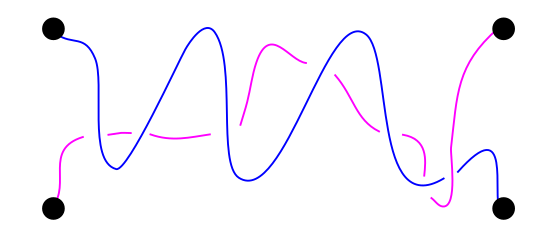
\includegraphics[width = 0.4\textwidth]{Inkscape Files/messy-strands.png} 
\end{center}
can easily be turned into the braid 
\begin{center}
	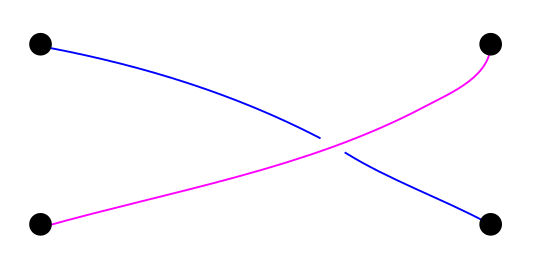
\includegraphics[width = 0.4\textwidth]{Inkscape Files/unmessy-strands.png}
\end{center}
just by nudging the blue strand up a bit and nudging the pink
strand down a bit. Maybe it would be a bit unfair or unproductive to say these
are different braids, simply because their strands do not strictly occupy the
same coordinates in space. But to speak about this precisely, we must make
precise what we mean by ``nudging.'' 

\begin{definition}[Homotopy]\label{homotopy}
   \begin{informal}
		The most basic form of a ``nudge'' is a \emph{homotopy}. To illustrate,
		suppose \(f\)  and \(g\) are functions that parameterize a line segment in
		\(\mathbb{R}^2\). So \(f, g\) can be a continuous functions \([0,
		1]\to\mathbb{R}^2\) as below in Figure \ref{2paths}: 
		\begin{figure}[!h]
		   \centering
			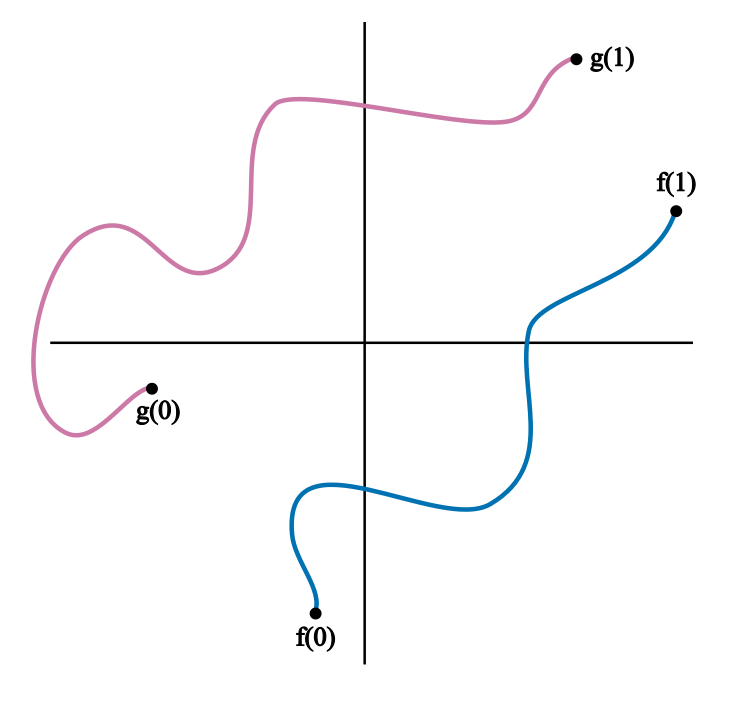
\includegraphics[width = 0.5\textwidth]{Inkscape Files/2lines.png}
			\caption{Continuous functions \(f, g: [0, 1]\to \mathbb{R}^2\)}
			\label{2paths}
		\end{figure}    

		We call these \textbf{paths} in \(\mathbb{R}^2\). Now let's say we want
		to ``nudge'' the path \(f\) to be the path \(g\). Intuitively, this is
		something we can do, say if \(f\) and \(g\) represent strings on a table.
		To express this mathematically, we must write a function that
		parameterizes the paths themselves.

		At time \(0\), the function must output the path \(f\), and at time
		\(1\), the function must output the path \(g\). All this must be done
		continuously, without skipping any space or breaking the strings, as
		below in Figure \ref{interpolated-paths}:
		\begin{figure}[!h]
		   \centering
			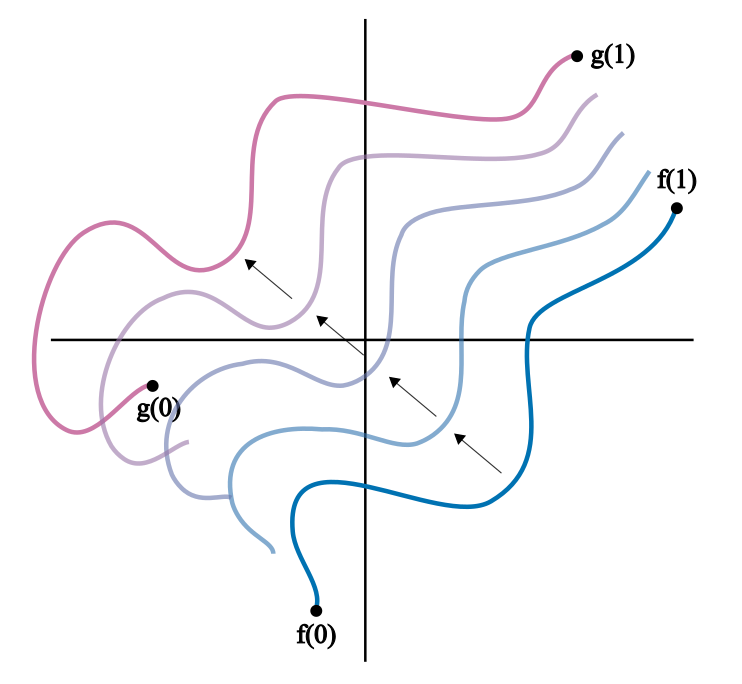
\includegraphics[width = 0.5\textwidth]
			{Inkscape Files/interpolated-paths.png}
			\caption{A homotopy from \(f\) to \(g\).}
			\label{interpolated-paths}
		\end{figure}

		Perhaps this is easier to do than it sounds. In this case, the function
		is given by \(F: [0,1]^2\to\mathbb{R}^2\) where for all \((s, t)\in[0,
		1]^2\), 
		\[
		   F(s, t) = f(s)(1-t) + g(s)t.
		\]
		Observe that at time \(t=0\), \(F(s, 0)\) gives the path \(f(s)\), and
		at time \(t=1\), \(F(s, 1)\) is the desired path \(g(s)\). As \(F\) is a
		sum of products of continuous functions, \(F\) is itself continuous, so
		no breaking or skipping occurs.
	\end{informal}
	\begin{formal}
	   Let \(U\subset \mathbb{R}^n\), \(V\subset\mathbb{R}^m\) be arbitrary
		subsets, and \(f, g: U\to V\) continous functions. A \textbf{homotopy}
		from \(f\) to \(g\) is a continuous function 
		\[
			F: U\times [0, 1]\to V
		\]
		such that 
		\begin{align*}
		   F(x, 0) = f(x),\\
			F(x, 1) = g(x).
		\end{align*}
		When such a homotopy exists, we say \(f\) and \(g\) are
		\textbf{homotopic}.

		To simply notation, we often denote \(F(x, t) = F_t(x)\) for all \(t\in
		[0, 1]\), where \(F_t\) is a function \(U\to V\).
	\end{formal}
\end{definition}

Moving forward, we assume all functions are continuous.
	
\begin{proposition}
	Let \(\sim\) denote the relation on functions \(U\to V\) where \(f\sim g\)
	if and only if there exists a homotopy from \(f\) to \(g\). Then \(\sim\) is
	an equivalence relation (Def. \ref{equivrel}).
\end{proposition}
\begin{proof}
	\begin{informal}
	   Homotopy behaves quite like equality, on many many levels. But it all
		starts with homotopy being an equivalence relation. Every function is
		homotopic to itself simply by a homotopy that keeps it still for all
		\(t\in[0, 1]\). Moreover, if \(f\) can be deformed to \(g\) by a
		homotopy, then it makes sense we can deform \(g\) back to \(f\) by
		reversing the motion. And, if we can deform \(f\) to \(g\), then \(g\) to
		\(h\), we can  \(f\) deform to \(h\) in the same time frame just by
		performing both deformations twice as fast in succession.
	\end{informal}

	\begin{formal} 
   We must prove \(\sim\) is reflexive, symmetric, and transitive.
	\begin{enumerate}[label=(\roman*)]
		\item To see \(\sim\) is reflexive, let \(f: U\to V\) be arbitrary. Then
		the function 
		\[
			F: U\times [0, 1]\to V
		\]
		defined by 
		\[
		   F(x, t) = f(x)
		\]
		is a homotopy from \(f\) to itself. Thus \(f\sim f\).

		\item To see \(\sim\) is symmetric, suppose we have \(f, g: U\to V\) such
		that \(f\sim g\). That is, there is
		a homotopy 
		\[
			F: U\times [0, 1]\to V.
		\] 
		Then we define 
		\[
			\overline{F}: U\times [0, 1]\to V
		\]
		by
		\[
		   \overline{F}(x, t) = F(x, 1-t).
		\] 
		Then
		\begin{align*}
			\overline{F}(x, 0) &= F(x, 1) = g(x),\\
			\overline{F}(x, 1) &= F(x, 0) = f(x)
		\end{align*}
		shows \(\overline{F}\) is indeed a homotopy from \(g\) to
		\(f\), so \(g\sim f\).

		\item To see \(\sim\) is transitive, suppose \(f, g, h: U\to V\) satisfy
		\(f\sim g\), \(g\sim h\). Then there exist 
		\[
			F, G: U\times [0, 1]\to V
		\]
		where \(F\) is a homotopy from \(f\) to \(g\) and \(G\) is a homotopy
		from \(g\) to \(f\). Then define 
		\[
			H: U\times [0, 1]\to V
		\]
		via
		\[
		   H(x, t) = 
			\begin{cases}
				F(x, 2t) &\text{if } 0\le t\le \frac{1}{2},\\
				G(x, 2t-1) & \text{if } \frac{1}{2}\le t\le 1.
		   \end{cases}
		\] 
		One can check \(H\) is a homotopy from \(f\) to \(h\), so \(f\sim h\).
	\end{enumerate}
\end{formal}
\end{proof}

	Since \(H\) is an equivalence relation, it is unambiguous to say \(f\) and
	\(g\) are homotopic if \(f\sim g\).

\begin{remark}
   For readers who know topology, the definition of homotopy
	extends to any maps \(f: X\to Y\). The other definitions in this section
	will also have natural topological generalizations.
\end{remark}

\begin{example}
	As may be evident from the discussion in Definition \ref{homotopy}, given
	any paths \(f, g: [0, 1]\to \mathbb{R}^2\), there is is a homotopy from
	\(f\) to \(g\) given by \(F: [0, 1]^2\to\mathbb{R}^2\), 
	\[
	   F(s, t) = f(s)(1-t) + g(s)t.
	\]
\end{example}

\begin{example}
	The existence of homotopies depends on the choice of
	codomain. Given the paths \(f, g: [0, 1]\to
	\mathbb{R}^2\setminus\{(0, 0)\}\) defined by 
	\begin{align*}
	   f(t) = (\sin(2\pi t), \cos(2\pi t)),\\
		g(t) = f(t) + (1, 1),
	\end{align*}
	pictured in Figure \ref{circles} below, there is no function
	that can move \(f\) to \(g\) without breaking or skipping at the origin.

	\begin{figure}[!h]
	   \centering
		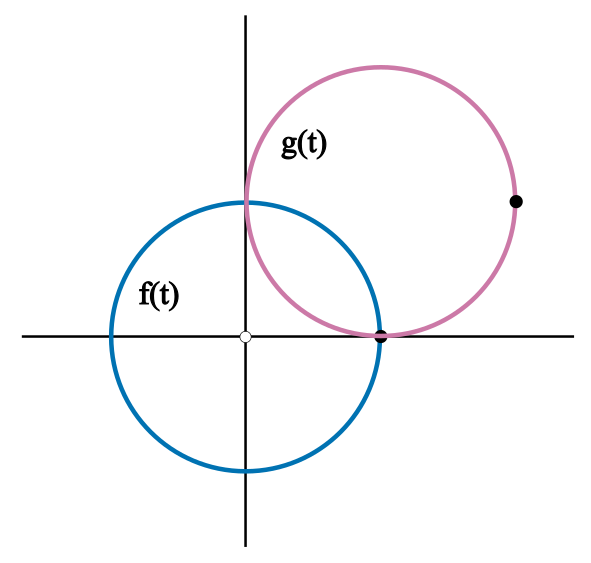
\includegraphics[width = 0.4\textwidth]{Inkscape Files/circles.png}
		\caption{\(f\) and \(g\) are homotopic as paths in \(\mathbb{R}^2\), but
		not as paths in \(\mathbb{R}^2\setminus\{(0, 0)\}\). There is no way to
		move \(f\) to \(g\) without \(f\) at the origin.}
		\label{circles}
	\end{figure}
\end{example}

\begin{example}\label{first-squishing}
    Here's a more interesting example. Let \(C\) denote the hollow cylinder
	 \(S^1\times [0, 1]\subset\mathbb{R}^3\). Let the functions \(\id:
	 C\to C\), \(r:C\to C\) be defined by 
	 \begin{align*}
	    \id(x, s) = (x, s),\\
		 r(x, s) = (x, 0).
	 \end{align*}
	 They are both continuous. 
	 Observe that \(r\) is collapsing all of \(C\) onto the base circle
	 \(S^1\times\{0\}\). We claim there is a homotopy from \(\id\) to \(r\).

	 Let \(F: C\times [0, 1]\to C\) be defined by 
	 \[
	    F((x, s), t) = (x, s(1-t)).
	 \] 
	 This function is continuous and indeed, 
	 \begin{align*}
		 F((x, s), 0) =
		 (x, s) = \id(x, s),\\
		 F((x, s), 1) = (x, 0).
	 \end{align*}
	 This gives \(r\) a nice physical interpretation. We can think of \(\id\) as
	 representing the cylinder \(C\) in its original state, not changing the
	 positions of any points. Then, to apply \(r\), we squish \(C\) down to a
	 circle in accordance to \(F\) until we reach \(r\). So \(r\) can be
	 interpreted squishing \(C\) down. This is pictured below in Figure
	 \ref{squishing}.
	 \begin{figure}[!h]
		 \centering
		 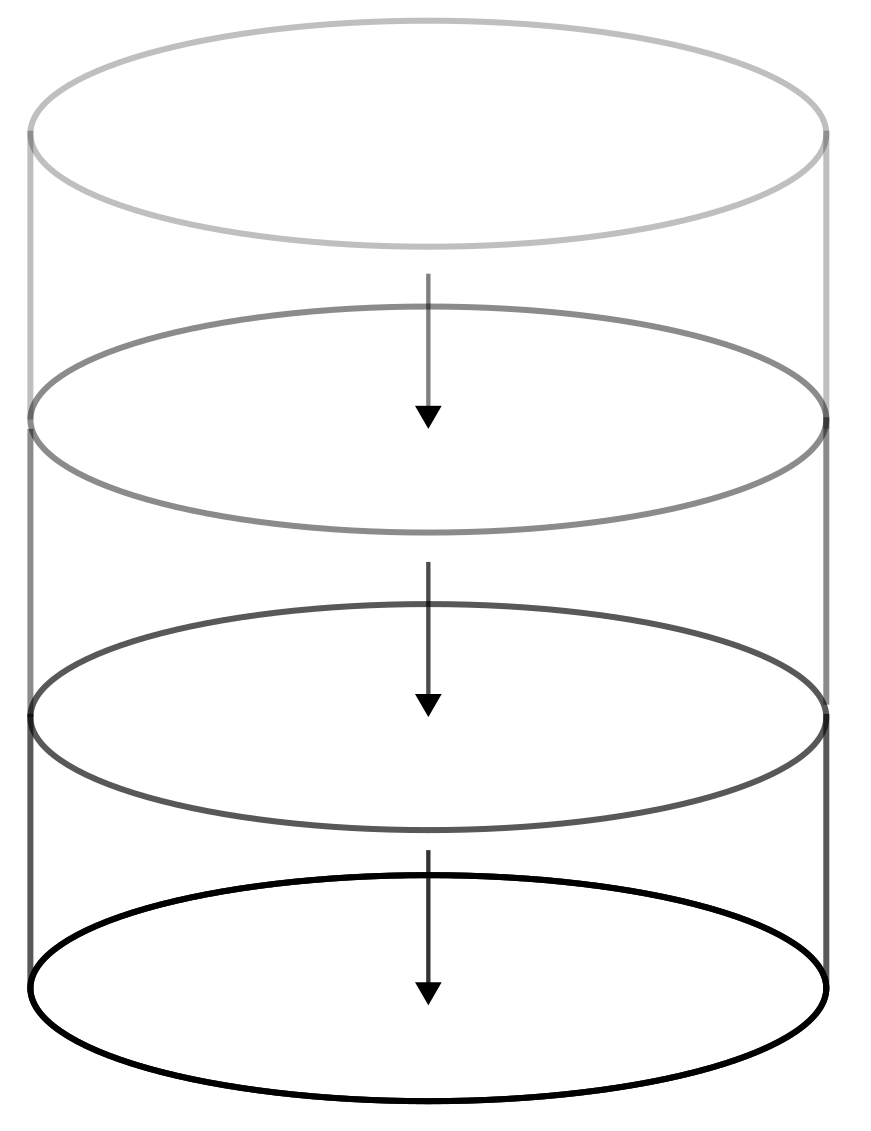
\includegraphics[width = 0.3\textwidth]{Inkscape Files/squishing.png}
		 \caption{Physical interpretation of \(r\) from Example
		 \ref{first-squishing} via the homotopy from \(\id\)
		 to \(r\). As time progresses from \(t=0\) to \(t=1\), we move the points
		 of \(C\) in accordance to where they are mapped by \(f\) until we get
		 \(r\).}
		 \label{squishing}
	 \end{figure}
\end{example}

We will set up some more terminology.
\begin{definition}
	Let \(U\subset\mathbb{R}^n, V\subset\mathbb{R}^m\), and let \(f: U\to V\) be a
	continuous function. If \(f\) is a  
	continuous function with a continuous inverse, we say \(f\) is a
	\textbf{homeomorphism}. If there is a homeomorphism
	between \(U\) and \(V\), we say \(U\) and \(V\) are \textbf{homeomorphic}
	and write \(U\cong V\).
\end{definition}

Like homotopy, homeomorphism defines an
equivalence relation. Hence, it is unambiguous to say two spaces are
homeomorphic.

\begin{example}
   Let \(U\subset\mathbb{R}^n\). The identity map \(U\to U\) is continuous and
	is its own
	inverse. Hence, it is a homeomorphism. We say \(U\cong U\), or \(U\) is
	homeomorphic to itself.
\end{example}

\begin{example}
   The function \(f: \mathbb{R}\to\mathbb{R}\) defined by \(f(x) = x^3\) is a
	homeomorphism because \(f^{-1}: \mathbb{R}\to\mathbb{R}\), \(f^{-1}(x) =
	x^{1/3}\) is continuous.
\end{example}

\begin{example}
   The function \(f: \mathbb{R}\to\mathbb{R}\) defined by \(f(x) = x^2\) is not
	a homeomorphism because \(f\) is not injective, hence has no inverse
	\(\mathbb{R}\to\mathbb{R}\).
\end{example}

\begin{example}\label{not-bicont}
	It is not true in general that if a function is continuous and invertible,
	that its inverse is continuous.
	For example define \(f: [0, 1)\to S^1\) via 
	\[
	   f(x) = (\cos(2\pi x), \sin(2\pi x))
	\] 
	(pictured in Figure \ref{circle-wrap}).

	\begin{figure}[!h]
	   \centering
		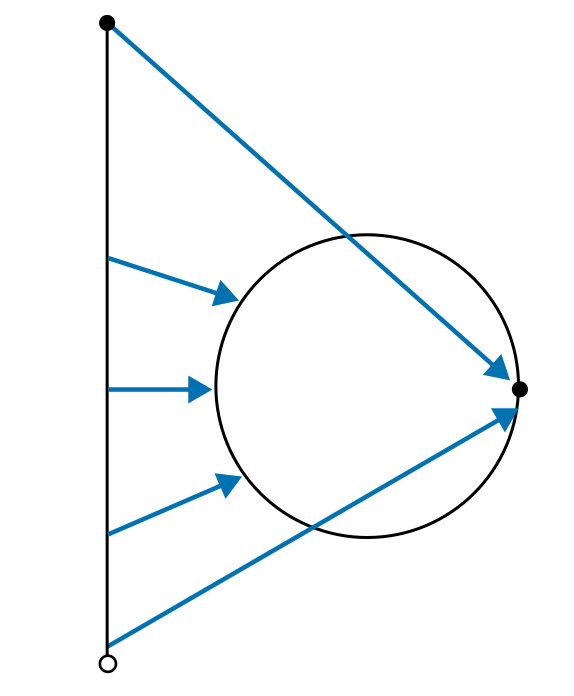
\includegraphics[width = 0.25\textwidth]{Inkscape Files/circlewrapping.png}
		\caption{\(f\) of Example \ref{not-bicont} is something like this.
		The interval \([0, 1)\) maps bijectively and continuously onto \(S^1\),
		but reversing this function will break \(S^1\).}
		\label{circle-wrap}
	\end{figure}

	Observe \(f\) wraps the interval
	\([0, 1)\) into a circle. This is
	continuous and
	bijective, hence invertible. However, the inverse requires the circle to
	taken to the interval \([0, 1)\). This breaks the circle, hence is not
	continuous.
\end{example}

\begin{definition}
  Let \(f: U\to V\) be a continuous function, and let \(W\subset V\) be the
  image of \(f\). If the function \(f:U\to W\) given by \(f\) is a
  homeomorphism, we call \(f\) an \textbf{embedding}.
\end{definition}

\begin{example}
   Embeddings are not as restrictive as homeomorphisms, but give more
	well-behaved functions than with just continuity. For example, the curve in
	Figure \ref{not-embedding} is continuous, but not an embedding. Likewise,
	the curves in Figure \ref{circles} are not embeddings (though they can be
	rewritten as embeddings \(S^1\to\mathbb{R}^2\)).

	Meanwhile, the curves of Figure \ref{2paths} are embeddings.
	\begin{figure}[!h]
	   \centering
		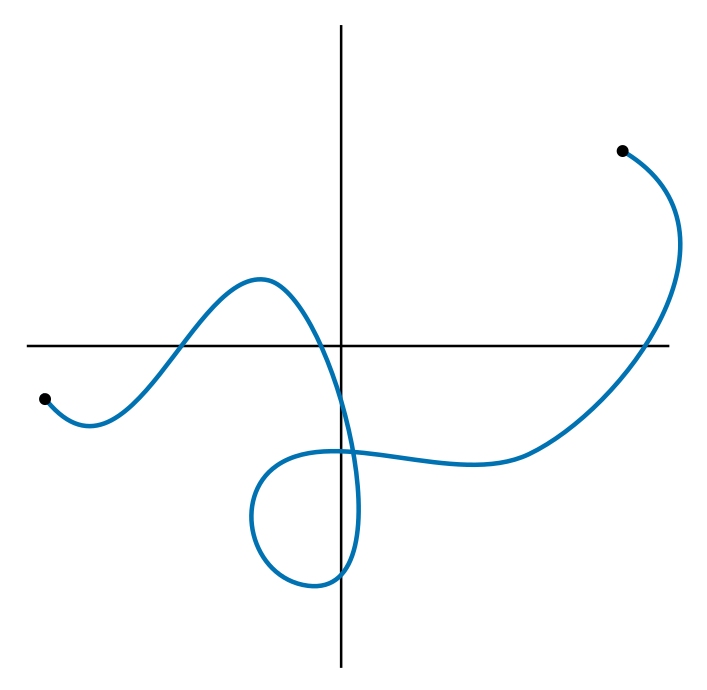
\includegraphics[width=0.4\textwidth]{Inkscape Files/not-embedding.png}
		\caption{Continuous, but not embedded path \([0, 1]\to\mathbb{R}^2\).}
		\label{not-embedding}
	\end{figure}
\end{example}

This allows us to define a stronger type of homotopy.
\begin{definition}
   Let \(U\subset\mathbb{R}^n\), \(V\subset\mathbb{R}^m\), and \(f, g: U\to V\)
	be embeddings. Then a homotopy \(F: U\times I\to V\) from \(f\) to \(g\) is
	an \textbf{isotopy} if \(F(s, t)\) is an embedding for all fixed \(t\in [0,
	1]\). If there is an isotopy between two embeddings, then we say they are
	\textbf{isotopic}.
\end{definition}
In short, an isotopy is a homotopy that is particularly nice.

Like homotopy and homeomorphisms, isotopy defines an equivalence relation.
Hence it is unambiguous to say two embeddings are isotopic.

\section{Introduction to Braids}\label{introduction-to-braids}
We are finally ready to study braids. We will see quickly that this study
puts to good use the accumulated knowledge of the previous sections.

\begin{definition}[Braid {\cite[p.~3]{mk1999}},	{\cite[p.~240]{primer}}]
	\label{braids}
	\begin{informal}
		To construct a mathematical braid with \(n\) strands,	pick \(n\)
		points on a disk in \(3\)-dimensional space. Then pick a parallel
		disk with the same distinguished points. We obtain a \textbf{braid on
		\(n\) strands} by drawing non-intersecting lines between the points
		on the two planes. The lines are not allowed to go backward.
	\end{informal}
	\begin{formal}
		Fix a positive integer \(n\). Let \(p_1, \ldots, p_n\) be points in the
		2-disk \(D^2\).
		A \textbf{braid on \(n\) strands}, or \textbf{n}-braid, is a collection
		of \(n\) paths \(f_i: [0,
		1]\to D^2\times [0, 1], 1\le i\le n\), called \textbf{strands}, and a
		permutation \(\overline{f}\in S_n\) such that each of the following holds: 
		\begin{enumerate}[label=(\roman*)]
			\item the strands \(f_i([0, 1])\) are disjoint,
			\item \(f_i(0) = (p_i, 0)\),
			\item \(f_i(1) = (p_{\overline{f}(i)}, 1)\),
			\item \(f_i(t)\in D^2\times\{t\}\) for all \(t\in[0, 1]\).
		\end{enumerate}
	\end{formal}
\end{definition}

Moving forward, we fix points \(p_1, \ldots, p_n\) for all positive integers
\(n\). We will assume every \(n\)-braid has these starting/ending points.
Moreover, when we say \(\beta = \{f_i : 1\le i\le n\}\) is an \(n\)-braid, we
will also use \(\beta\) to mean the subset of strands in \(D^2\times[0, 1]\)
given by \(\beta\). Therefore, if we have a function \(f\) whose domain is
\(D^2\times[0, 1]\), the expression \(f(\beta)\) makes sense.

To simplify notation, we will denote \(\mathbb{D} =
D^2\times[0, 1]\).

\begin{example}
	In Figure \ref{3-braids}, we have two examples of braids on \(3\) strands,
	which we refer to as \(3\)-braids. These braids are a subset of the
	cylinder formed by the parallel disks, or \(\mathbb{D}\). Moving
	forward, we omit the disks in figures.

	\begin{figure}[!h]
		\begin{subfigure}{.5\textwidth}
			\centering
			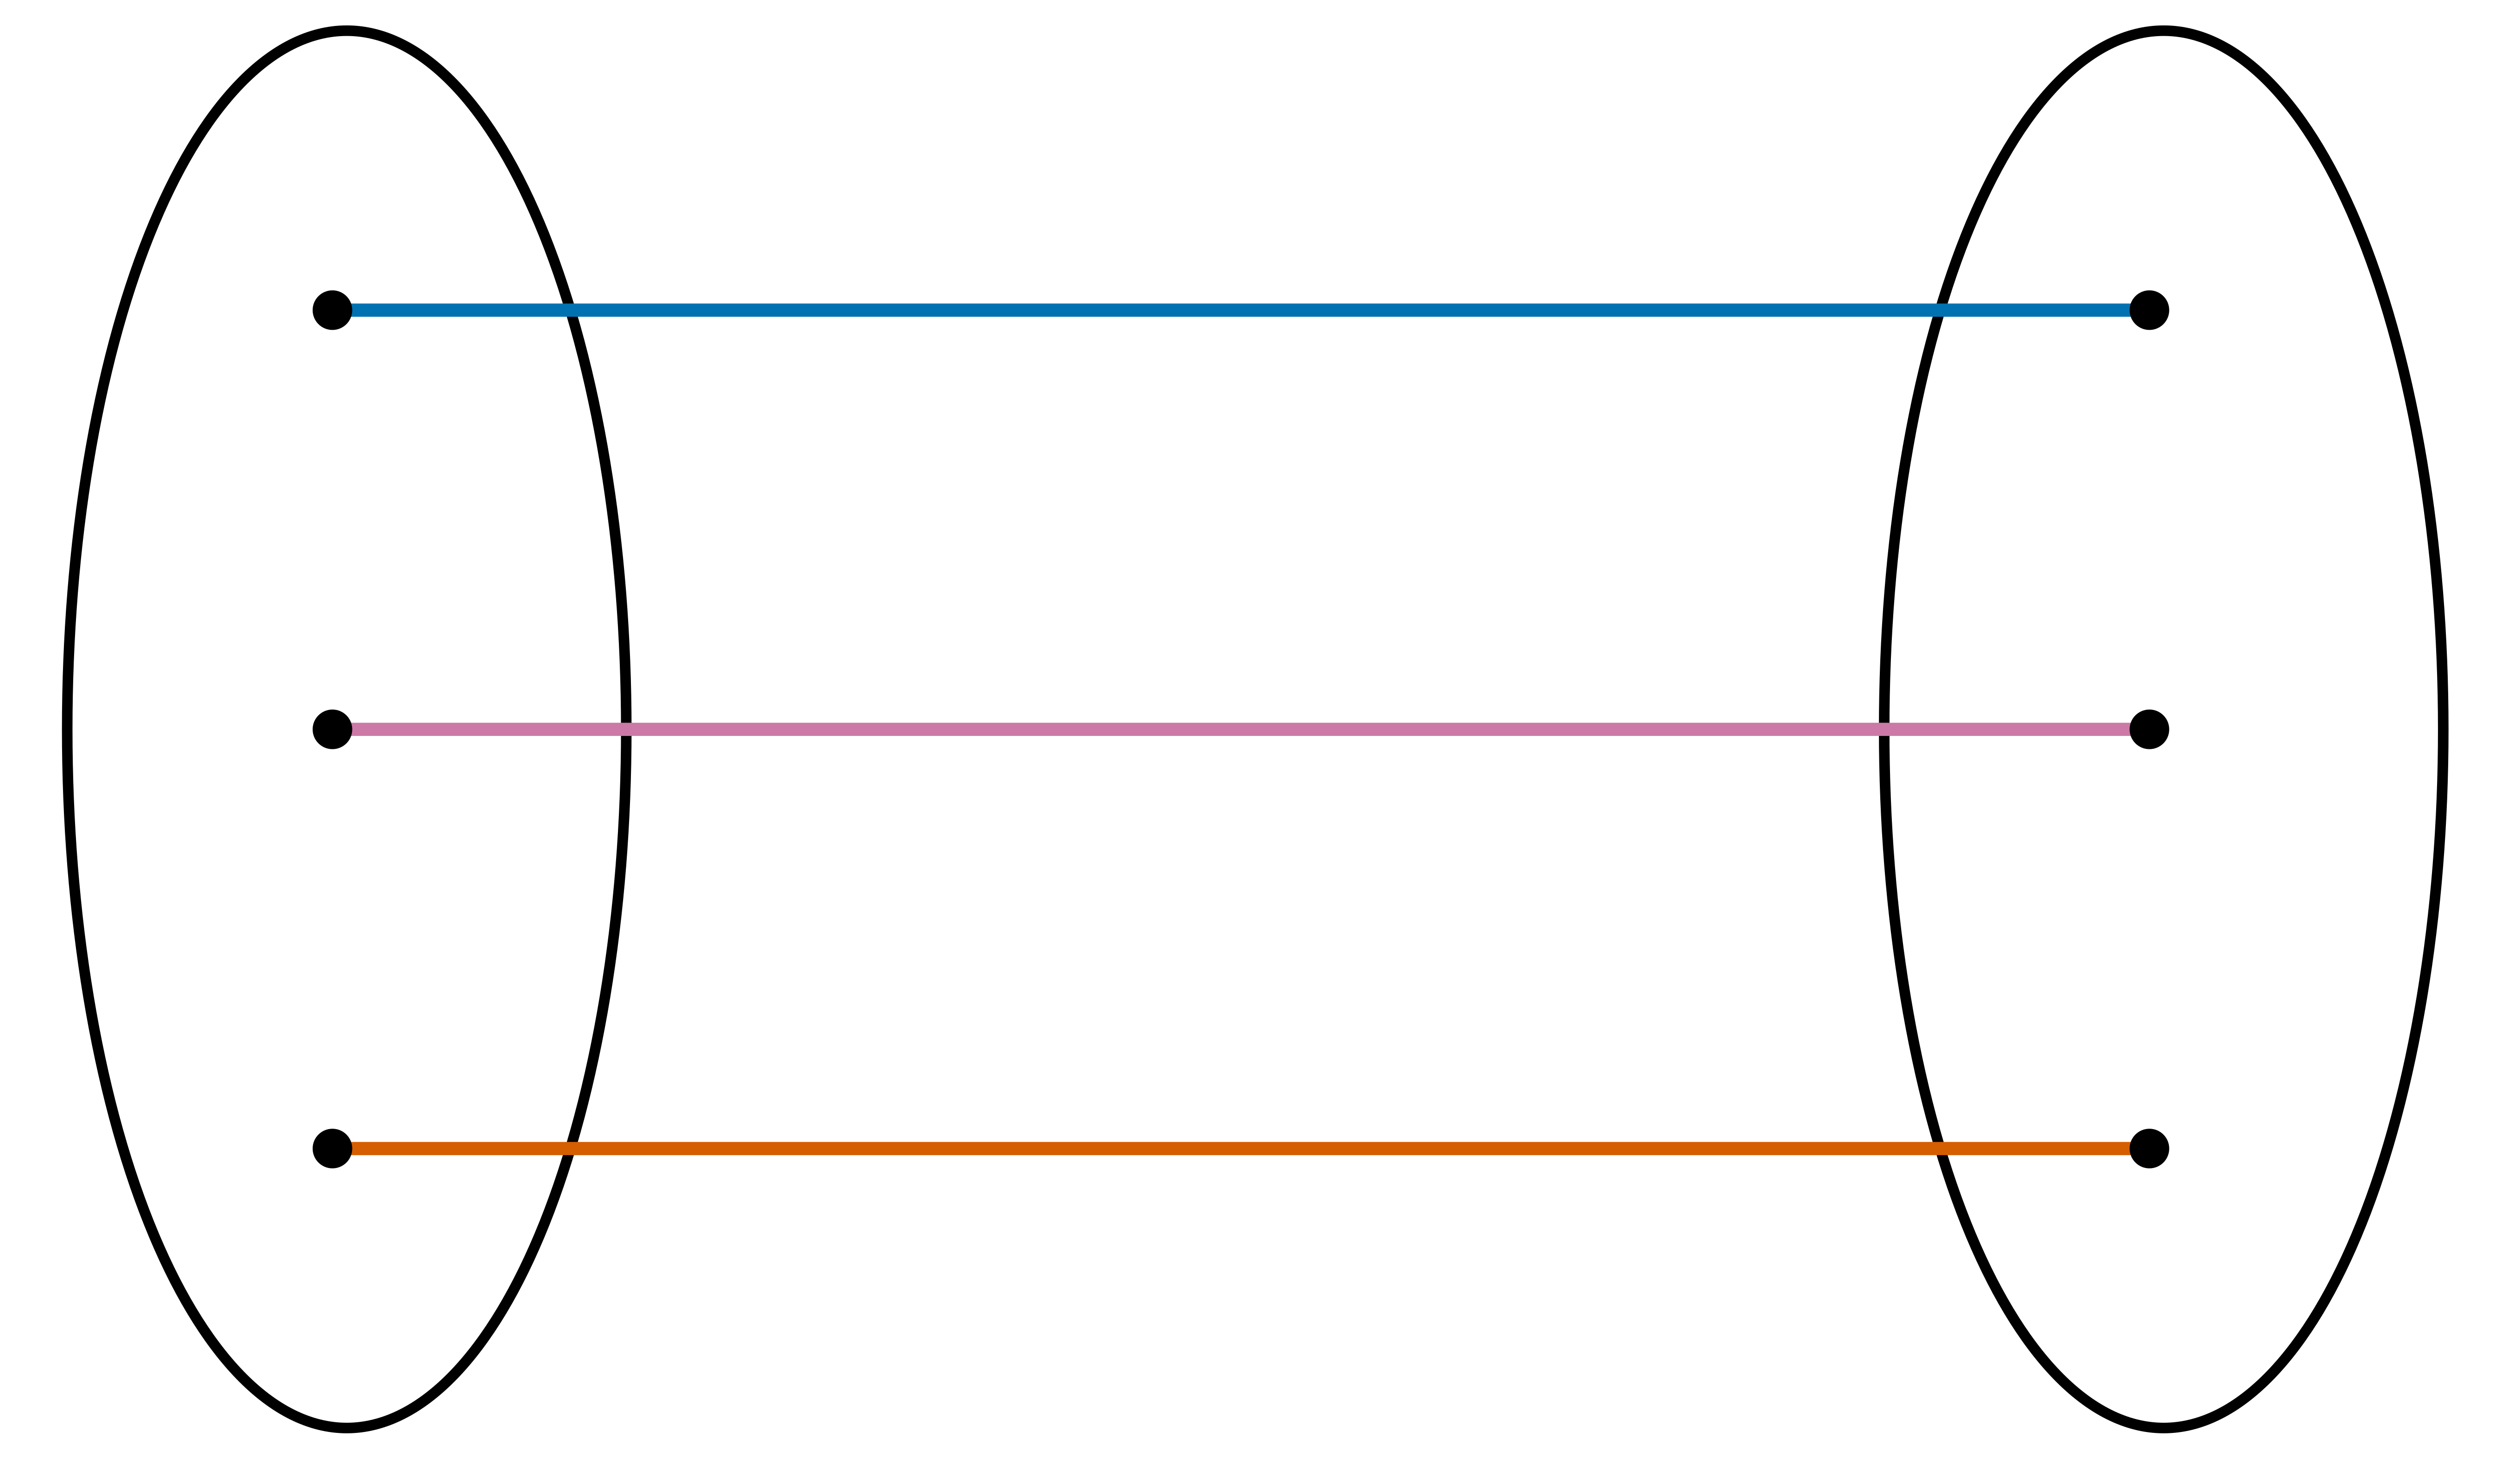
\includegraphics[width=.9\linewidth]{Inkscape Files/identityonthree.png}
			\caption{}
		\end{subfigure}%
		\begin{subfigure}{.5\textwidth}
			\centering
			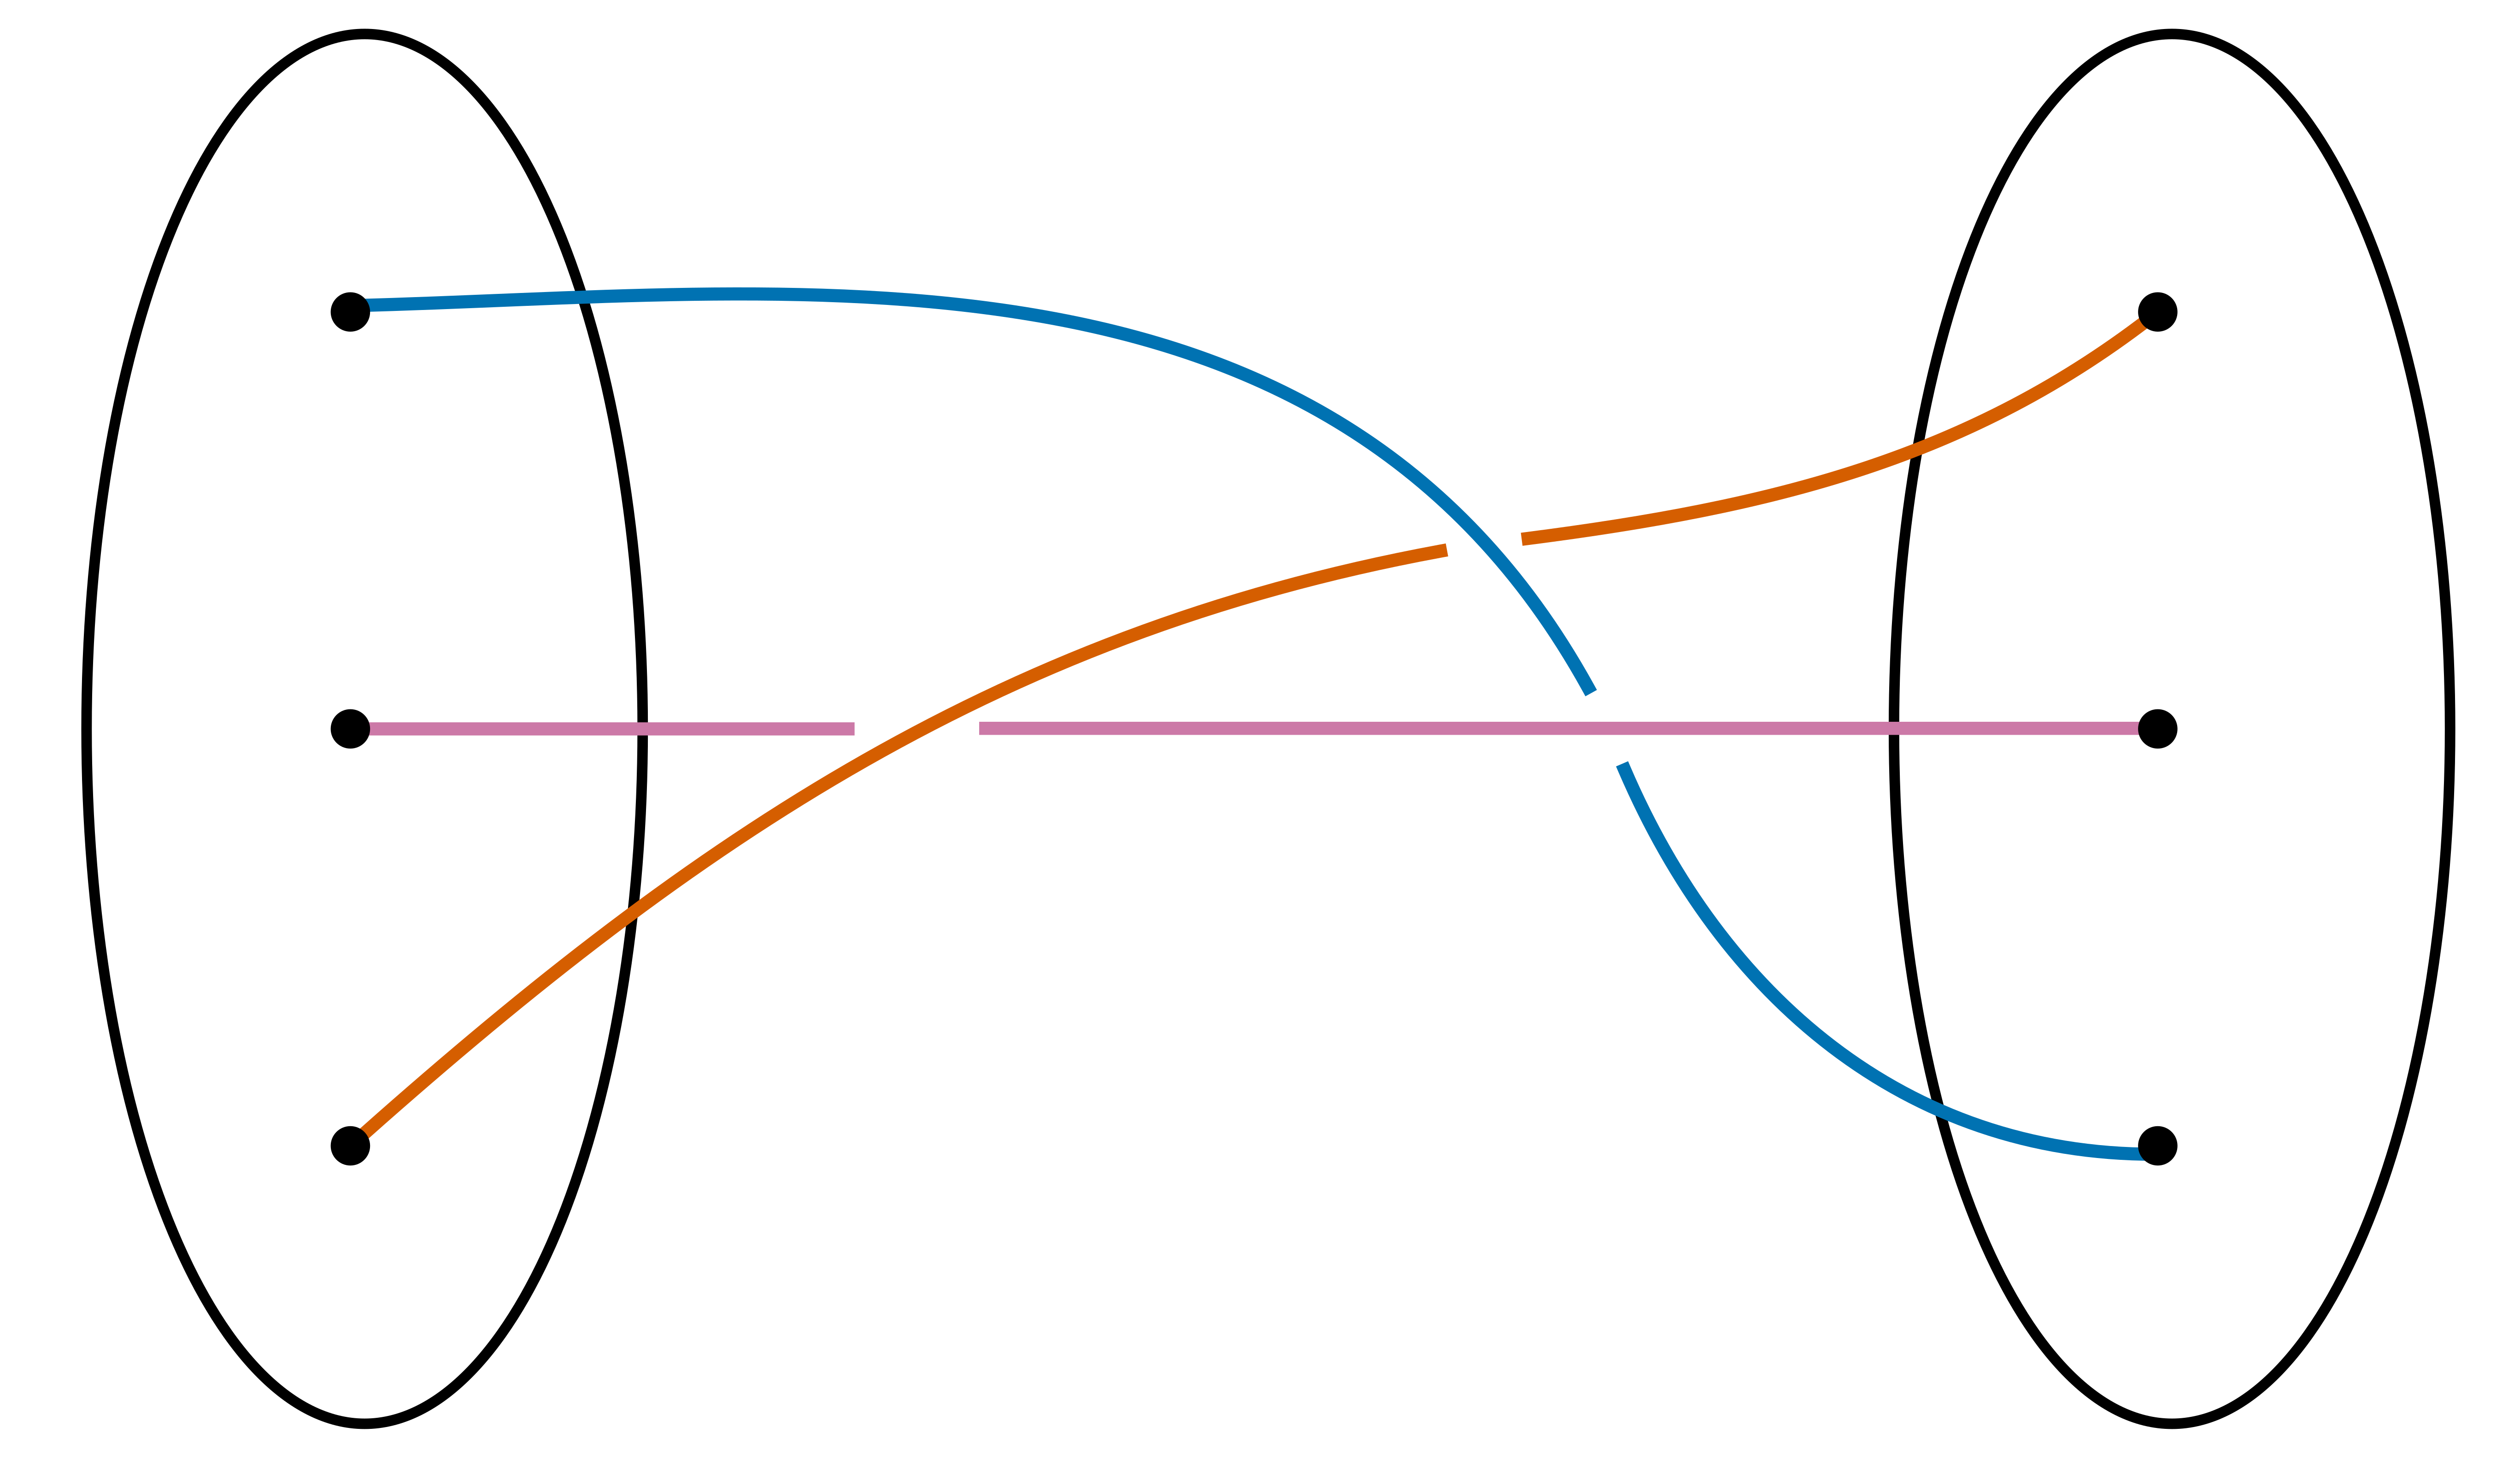
\includegraphics[width=.9\linewidth]{Inkscape Files/threebraid1.png}
			\caption{}
		\end{subfigure}%
		\caption{(a): On the left, we have what's technically a braid on 3
		strands. We can describe this by the paths \(f_i(t) = p_i\) for all
		\(t\in [0, 1]\). (b): On the right, a slightly more interesting braid on
		3 strands.}
		\label{3-braids}
	\end{figure}
\end{example}

\begin{example}
	In Figure \ref{falsebraids}, we have three non-example of braids.
	\begin{figure}[!h]
		\begin{subfigure}{.33\textwidth}
			\centering
			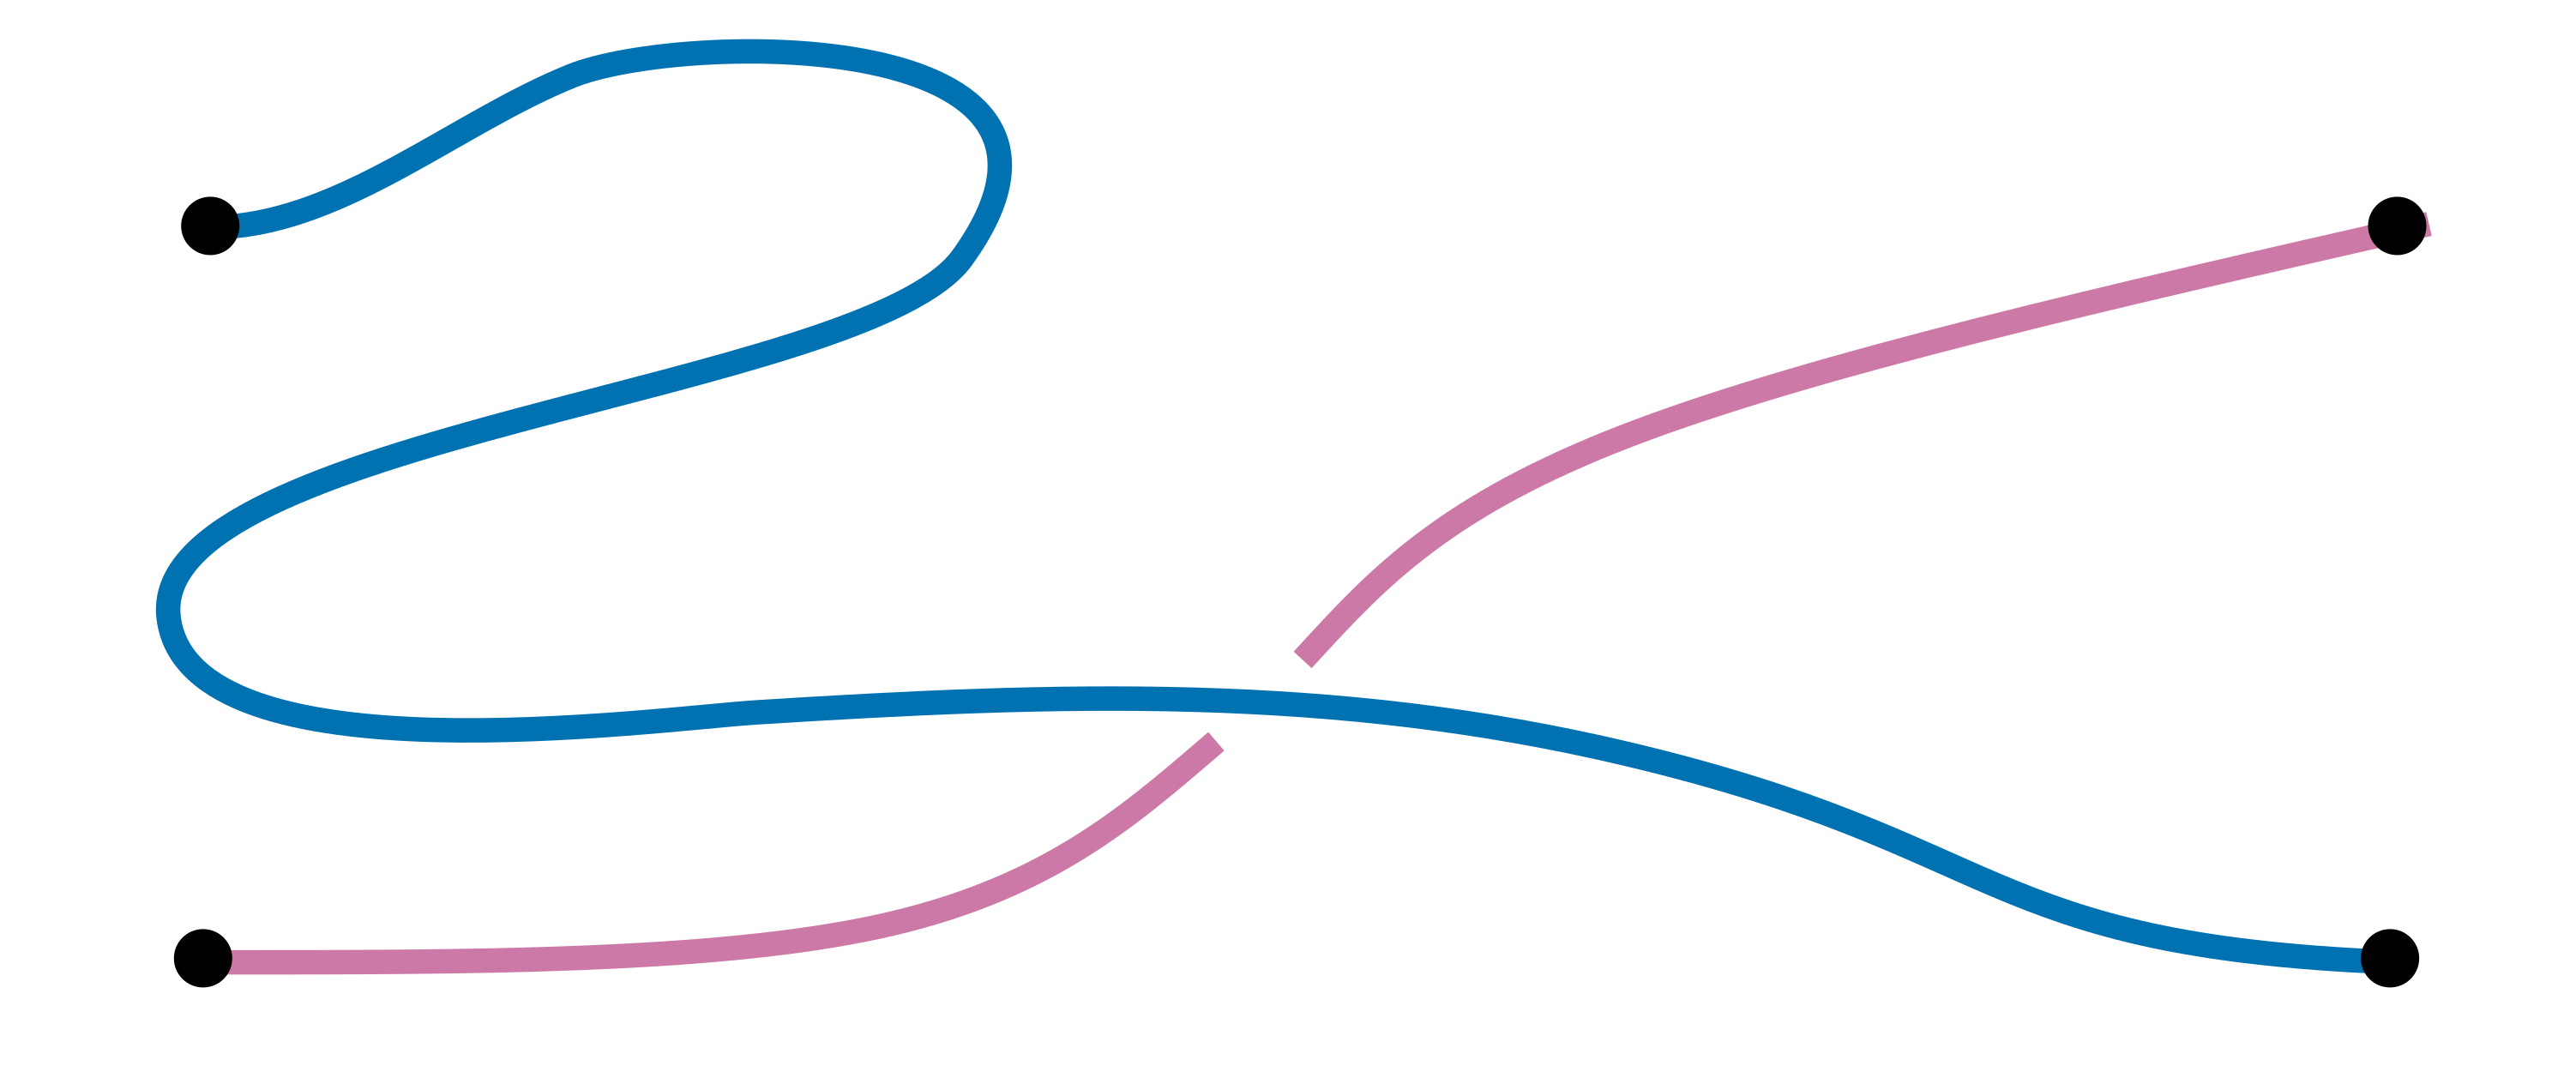
\includegraphics[width=.9\linewidth]{Inkscape Files/notbraid.png}
			\caption{}
		\end{subfigure}%
		\begin{subfigure}{.33\textwidth}
			\centering
			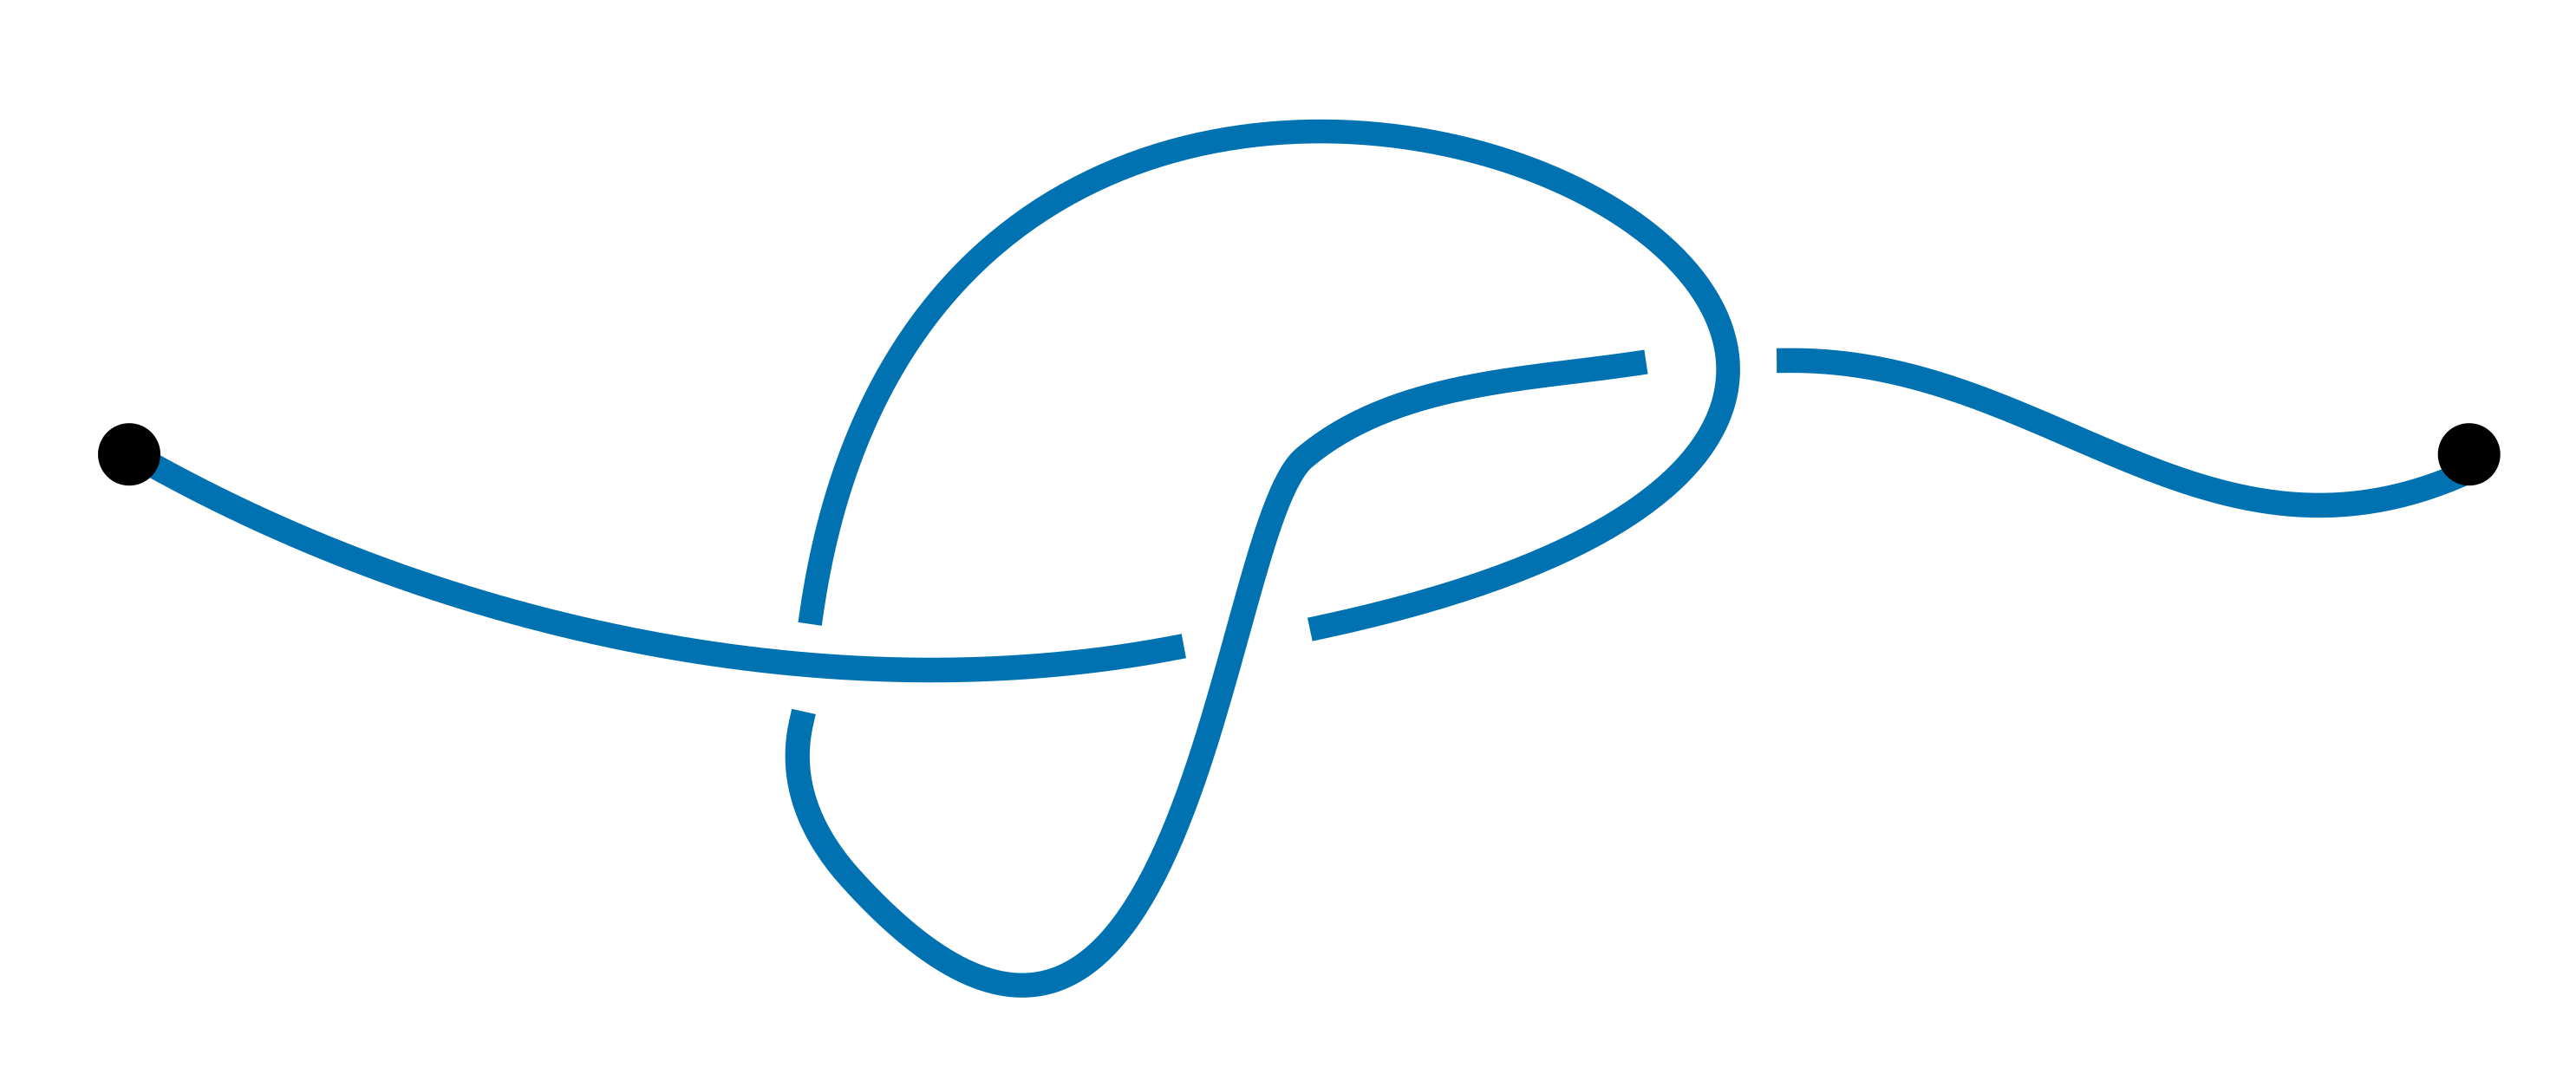
\includegraphics[width=.9\linewidth]{Inkscape Files/fancynotbraid.png}
			\caption{}
		\end{subfigure}%
		\begin{subfigure}{.33\textwidth}
			\centering
			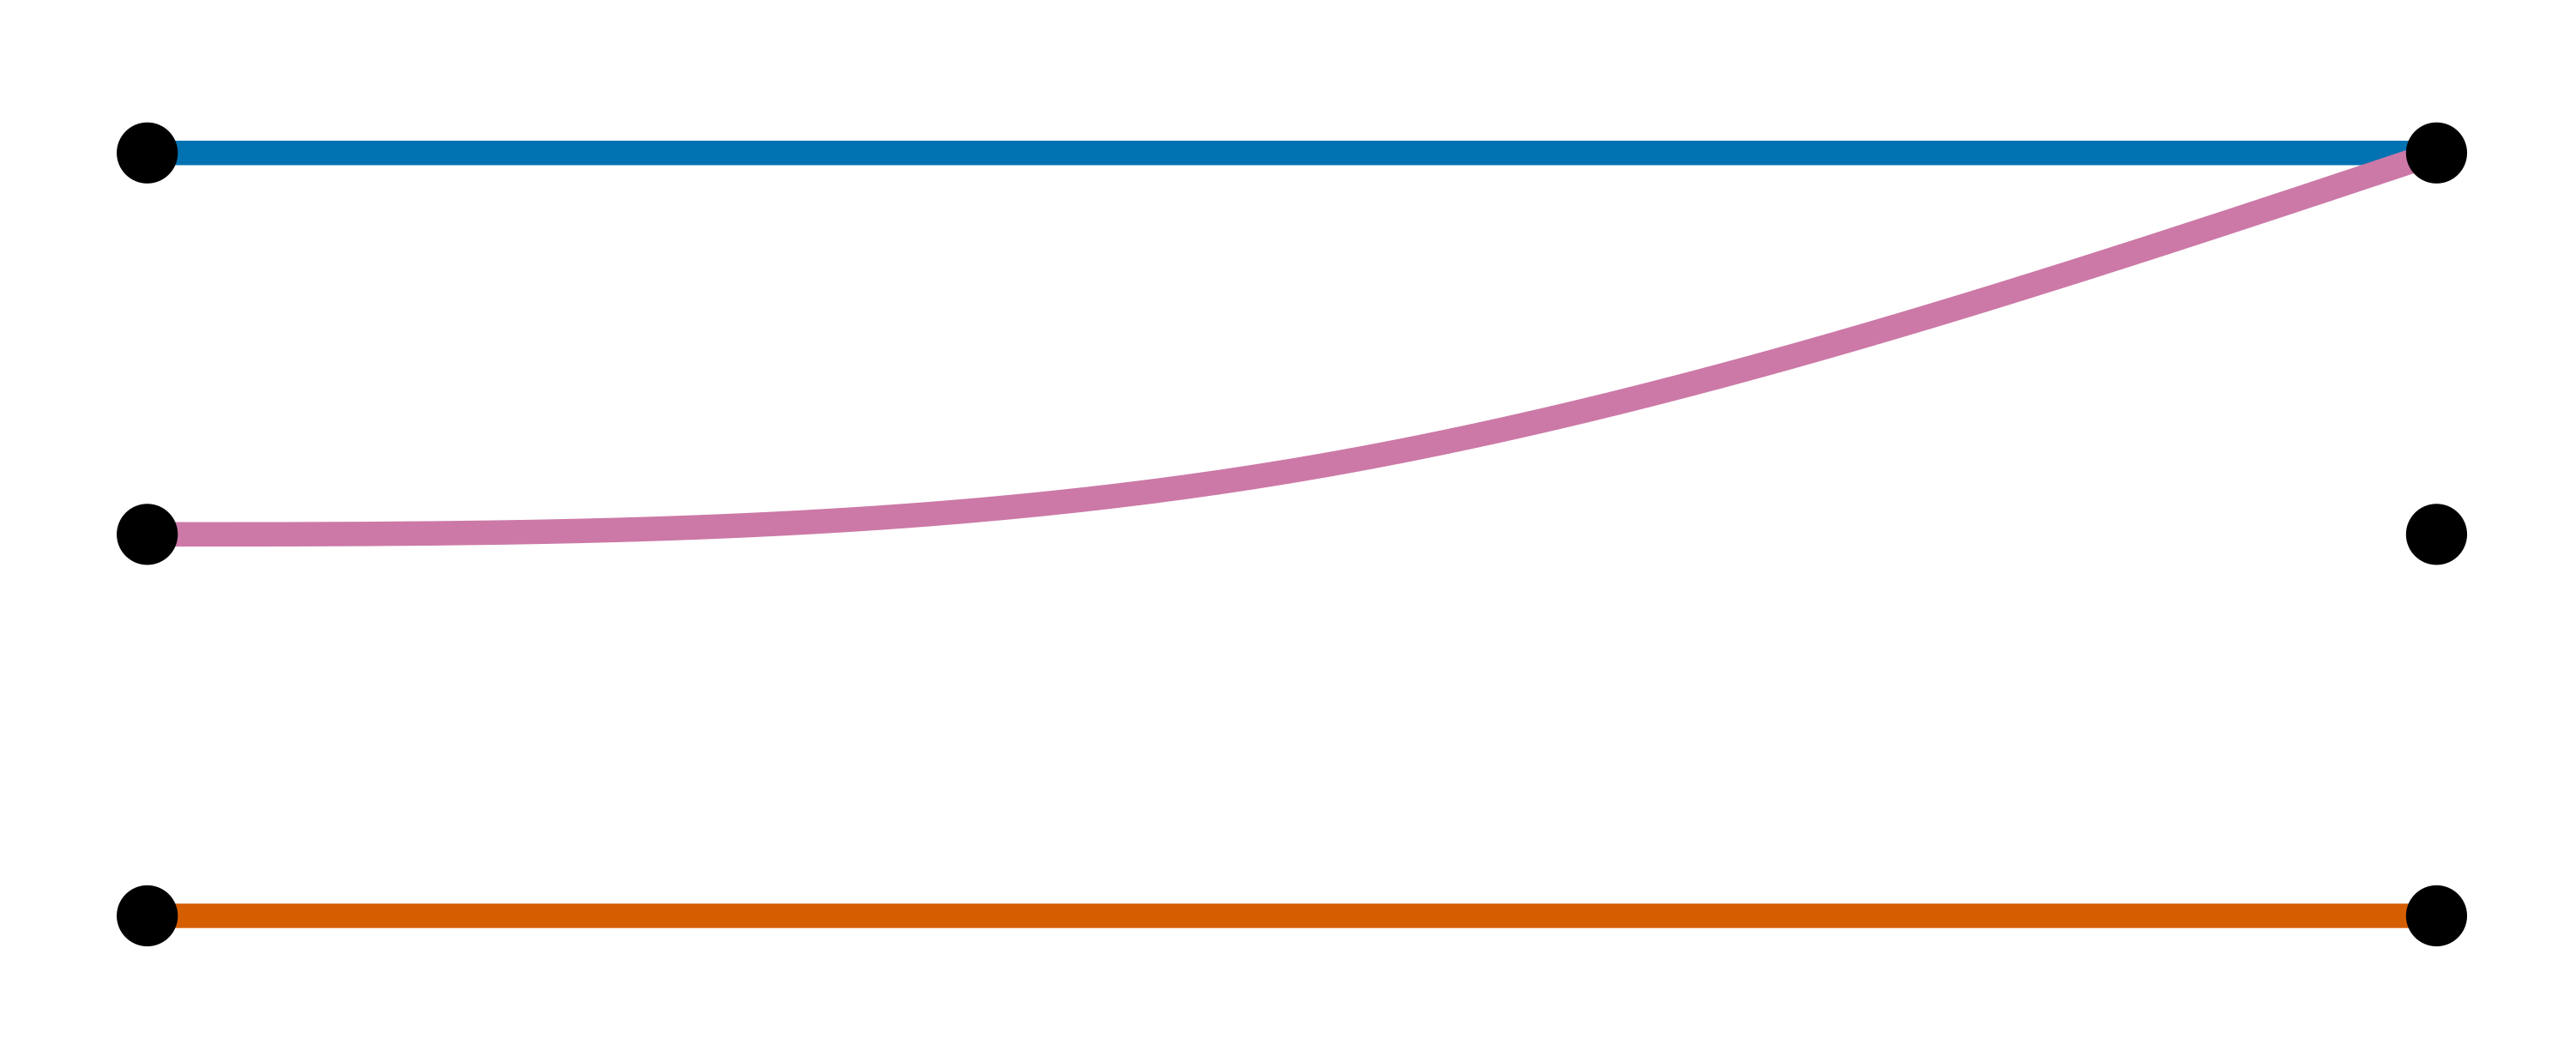
\includegraphics[width=.9\linewidth]{Inkscape Files/notbraid2.png}
			\caption{}
		\end{subfigure}
		\caption{(a) and (b) are not braids because they turn back on theselves. (c)
		is not a braid because the points are not permuted.}
		\label{falsebraids}
	\end{figure}
\end{example}

\begin{definition}[Braid equivalence
	{\cite[p.~96]{mk1999}}]\label{equivalentbraids}
	\begin{informal}
	   We want to say two braids are the same if we can pull the strands around
		so that they are equal. For example, we want to say the three braids in
		Figure \ref{equiv-2-braids} are the same. The rules are, strands cannot
		cross each other
		and the starting/ending points cannot change. They are like infinitely
		elastic rubber bands.
		\begin{figure}
			\begin{subfigure}{.33\textwidth}
				\centering
				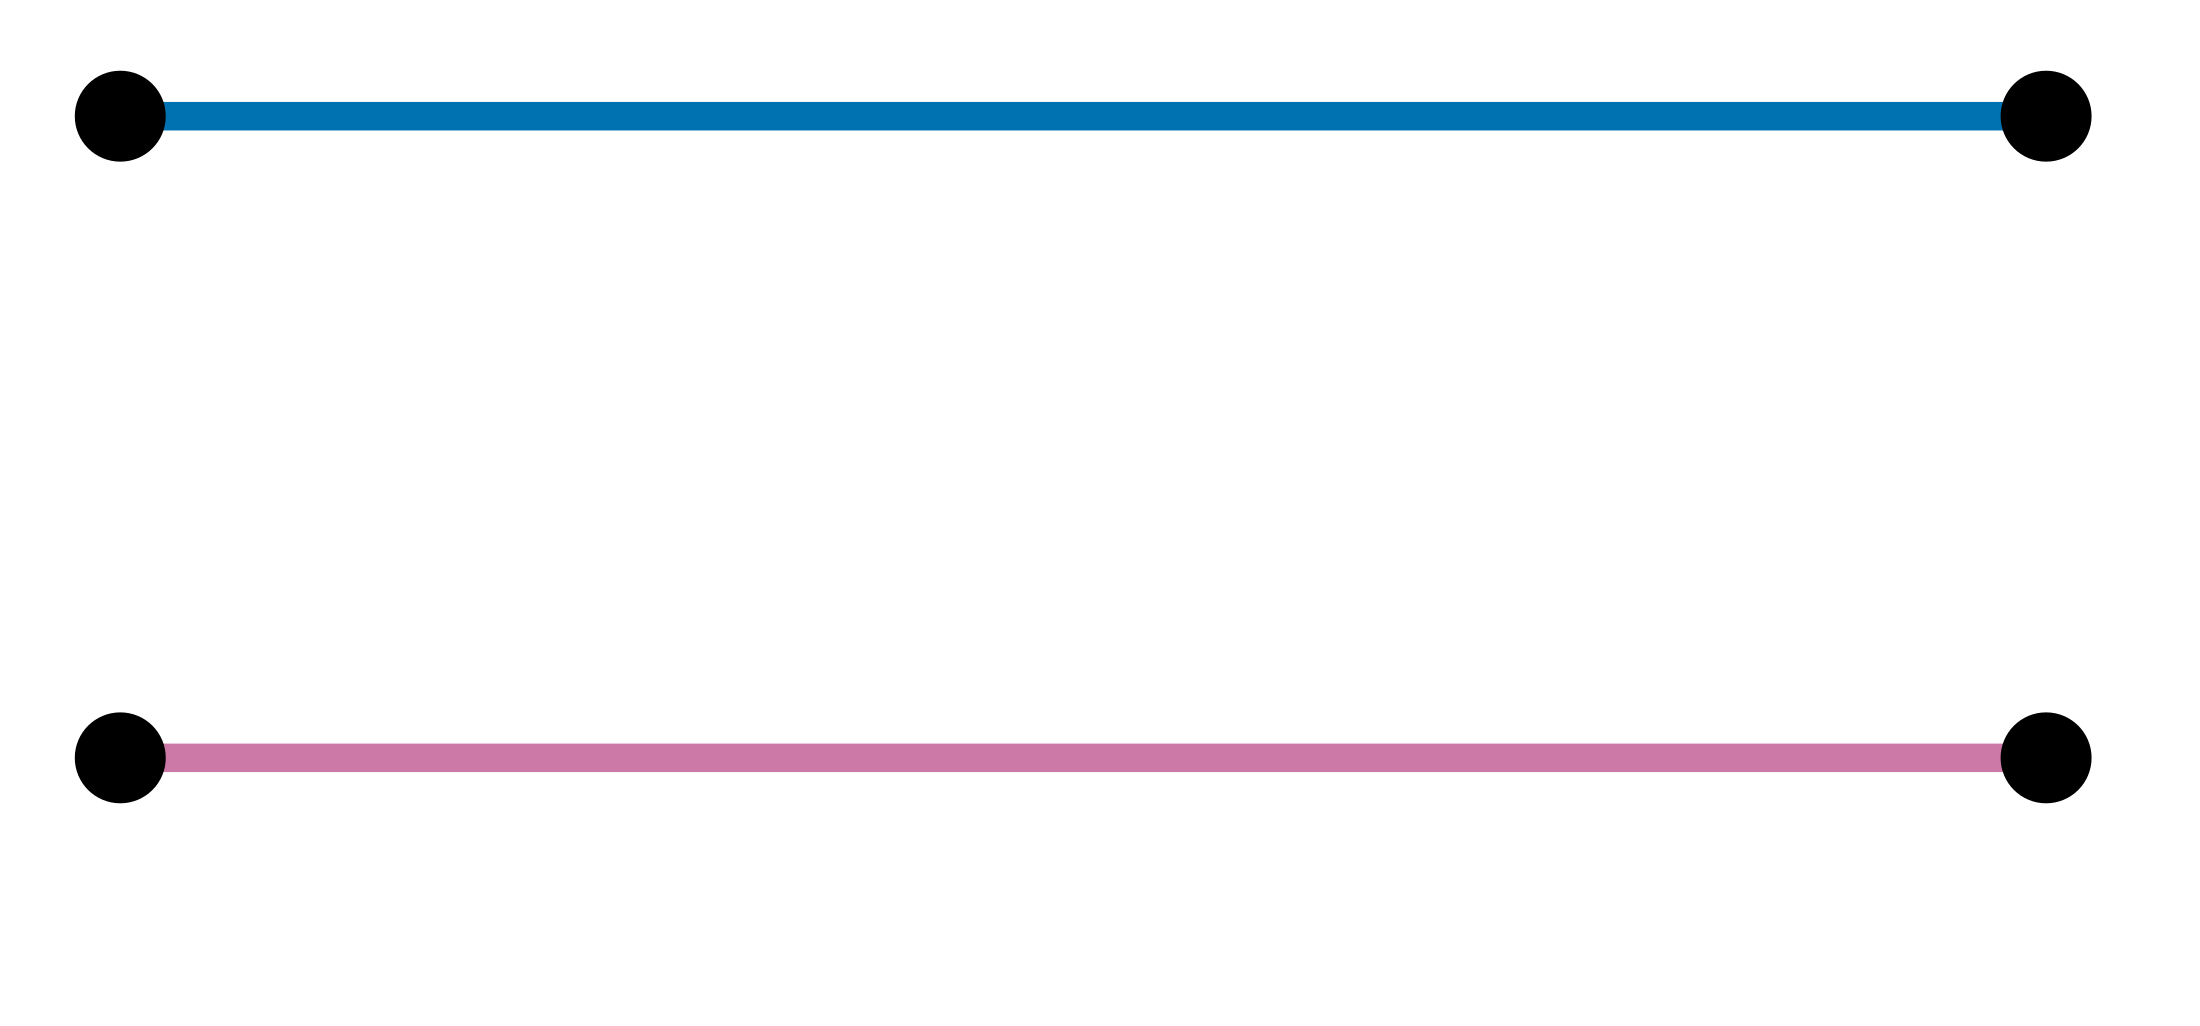
\includegraphics[width=.9\linewidth]{Inkscape Files/identityontwo.png}
			\end{subfigure}%
			\begin{subfigure}{.33\textwidth}
				\centering
				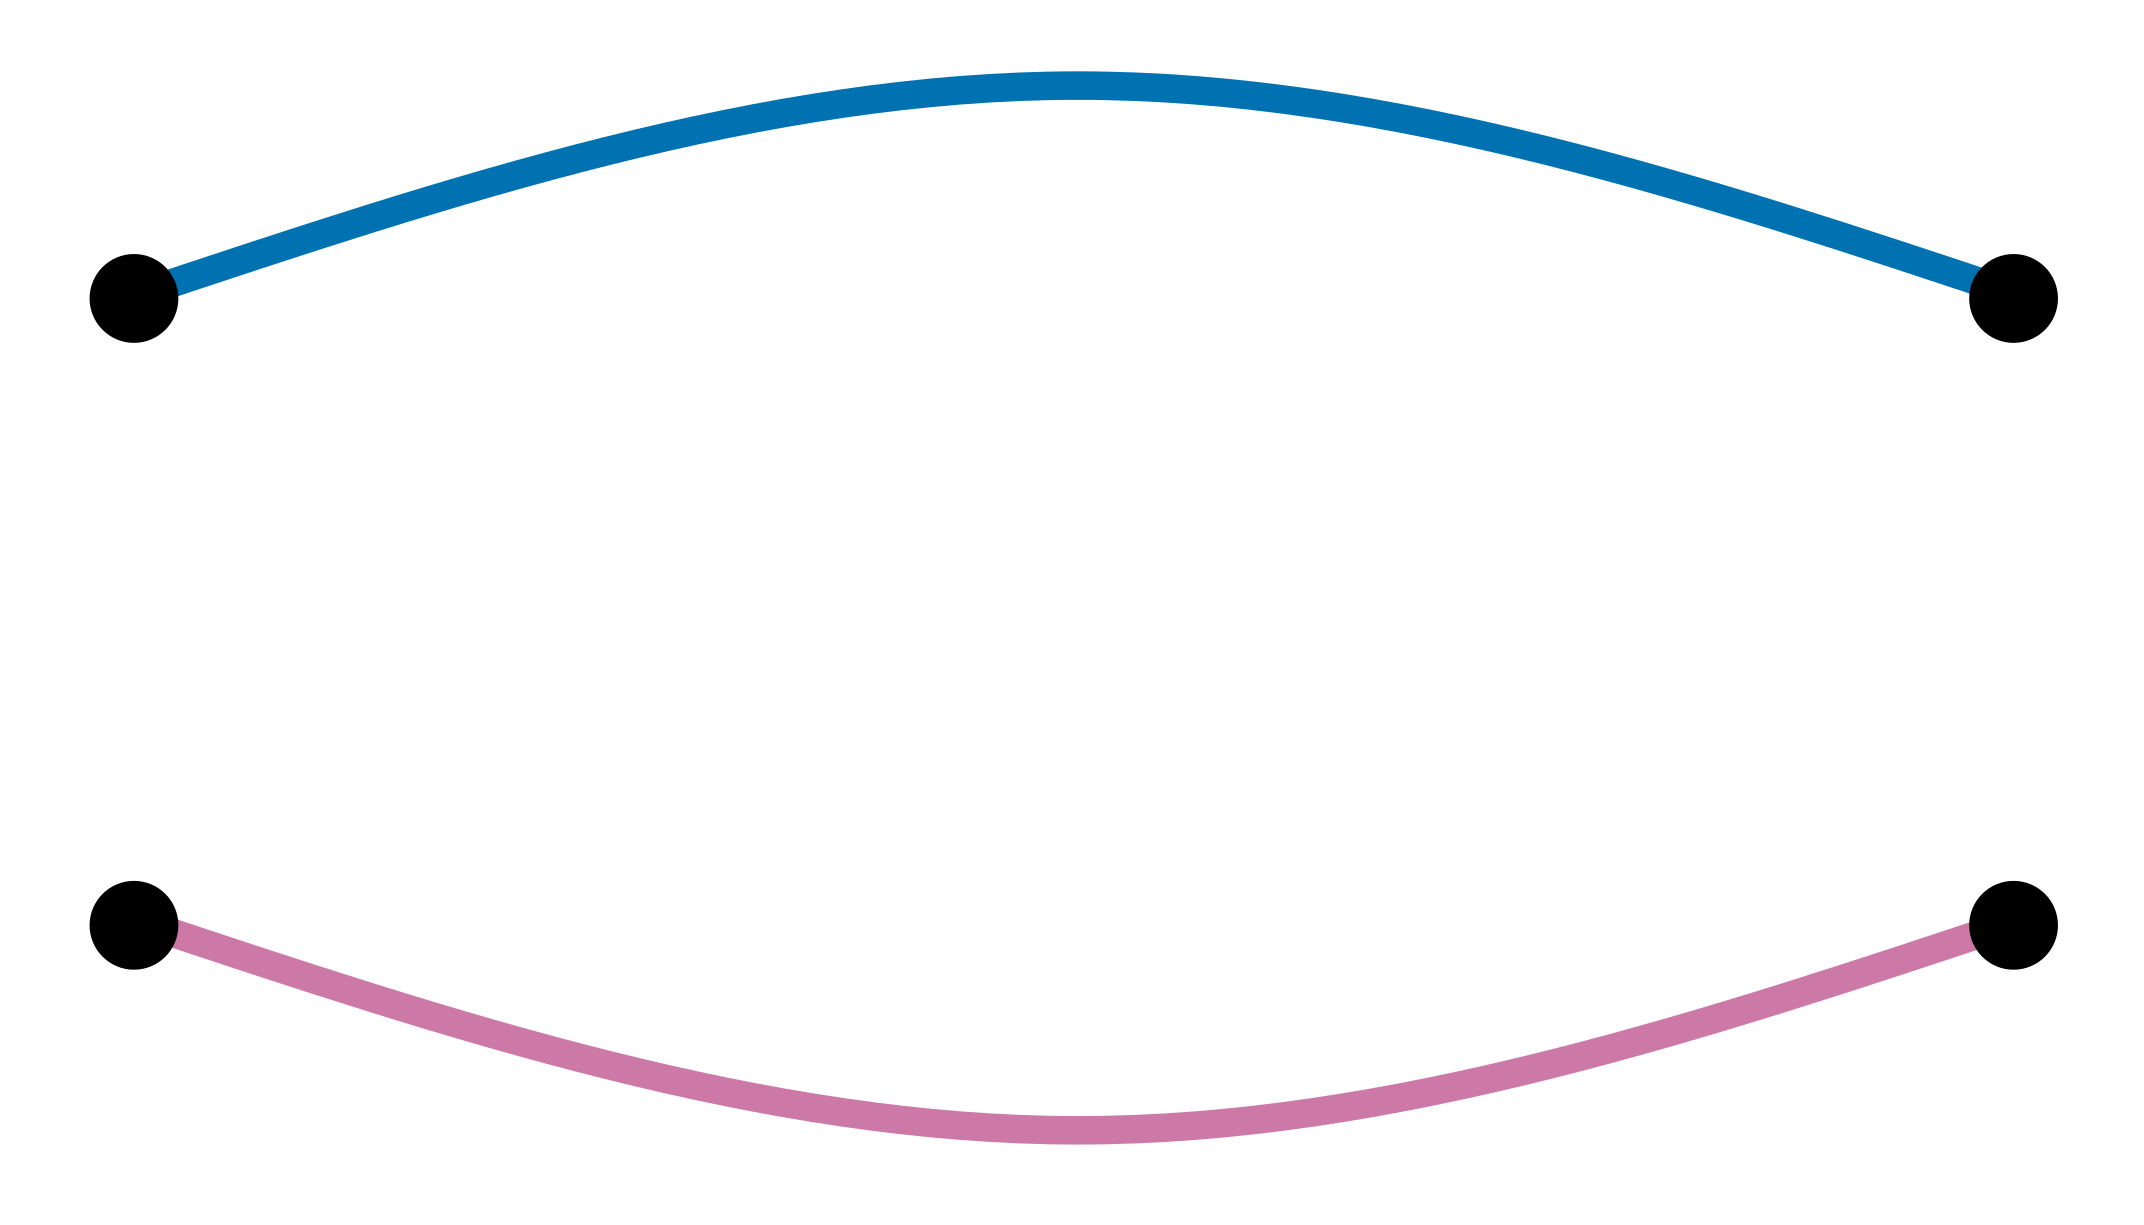
\includegraphics[width=.9\linewidth]{Inkscape
				Files/identityontwo2.png}
			\end{subfigure}%
			\begin{subfigure}{.33\textwidth}
				\centering
				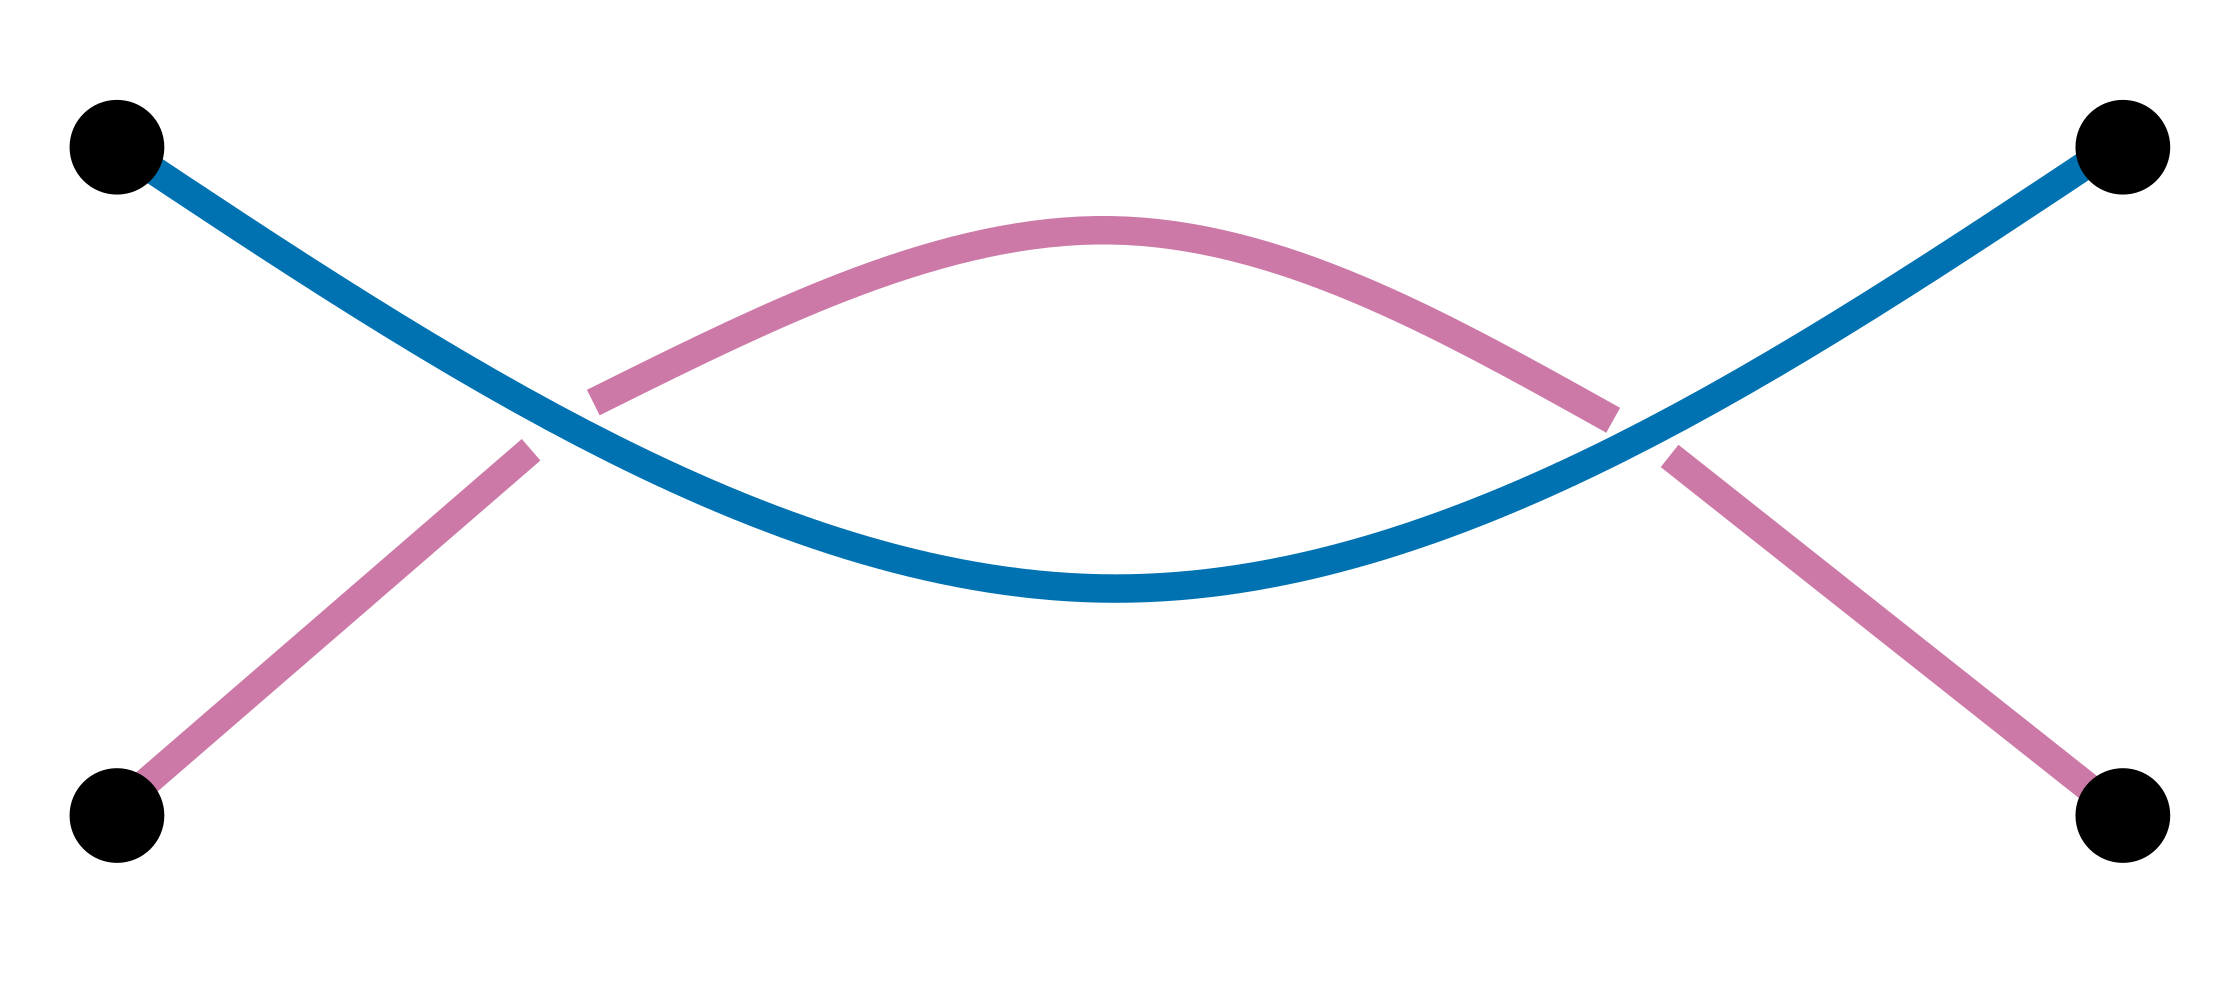
\includegraphics[width=.9\linewidth]{Inkscape
				Files/identityontwo3.png}
			\end{subfigure}
			\caption{These three 2-braids are equivalent.}
			\label{equiv-2-braids}
		\end{figure}
	\end{informal}
	\begin{formal}
		Denote \(\mathbb{D} = D^2\times[0, 1]\). We declare two braids \(\beta\)
		and \(\beta'\) \textbf{equivalent}
		if there	exists a continuous map 
		\[
			h: \mathbb{D}\times[0, 1]\to\mathbb{D}
		\]
		such that: 
		\begin{enumerate}[label=(\roman*)]
			\item for all \(t\in[0, 1]\), \(h_t:\mathbb{D}\to\mathbb{D}\) is a
			homeomorphism,
			\item for all \(t\in[0, 1]\), \(h_t\) is the identity on the 
			cylindrical boundary of \(\mathbb{D}\). That is, \(h_t\) fixes
			the boundary pointwise.
			\item \(h_0\) is the identity and \(h_1(\beta) = \beta'\). We call \(h\)
			an \textbf{ambient isotopy}. 		
		\end{enumerate} 
	\end{formal}
\end{definition}
An ambient isotopy is even stronger than an isotopy. In the previous definition
(Def. \ref{equivalentbraids}), we obtain an isotopy from \(\beta\) to
\(\beta'\) by hitching a ride on an isotopy of homeomorphisms of the entire
space \(\mathbb{D}\). It is quite strict, but the ambient isotopy is equivalent
to the intuitive notion of pulling and nudging the strands without breaking
them or crossing them through each other.

\begin{comment}
   In truth, I do not know why an ambient isotopy is required as opposed to
	simply an isotopy of the map \(\beta :\{p_1, \ldots,
	p_n\}\times I\to\mathbb{D}\) that fixes the endpoints. Although I understand
	how all knots can be isotoped to the unknot, I have not seen similar
	arguments for braids. If anyone has an explanation or counterexample, I
	would very grateful to hear it!
\end{comment}

\begin{remark}
   There is also a much more easy notion of braid equivalence formulated in
	terms in elementary moves. It takes no fancy math to understand, and the
	interested reader can find it in {\cite[p.~4]{mk1999}}.
\end{remark}

\begin{example}
	The braids in Figure \ref{equivalent4braids} are equivalent.
	\begin{figure}[h]
		\begin{subfigure}{.5\textwidth}
			\centering
			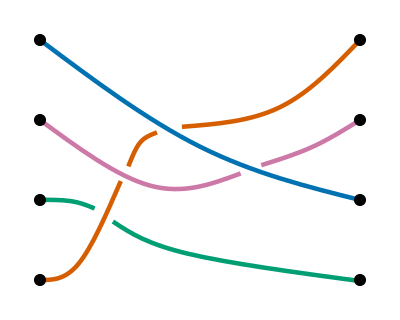
\includegraphics[width=.9\linewidth]{Inkscape Files/4braid1.png}
			\caption{}
		\end{subfigure}%
		\begin{subfigure}{.5\textwidth}
			\centering
			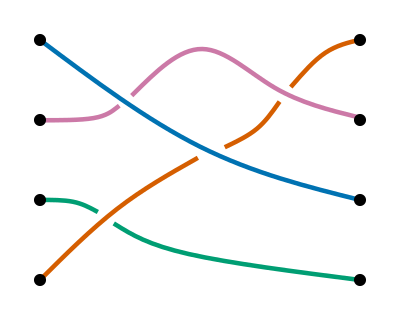
\includegraphics[width=.9\linewidth]{Inkscape Files/4braid2.png}
			\caption{}
		\end{subfigure}
		\caption{These 4-braids are equivalent. From (a), shift the pink line upward
		and nudge the orange line down to get (b).}
		\label{equivalent4braids}
	\end{figure}
\end{example}

\begin{example}
 	The braids in Figure \ref{unequal2braids} are not equivalent. 
	\begin{figure}[h]
		\begin{subfigure}{.5\textwidth}
			\centering
			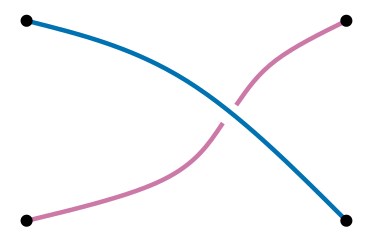
\includegraphics[width=.9\linewidth]{Inkscape Files/2braid.png}
		\end{subfigure}%
		\begin{subfigure}{.5\textwidth}
			\centering
			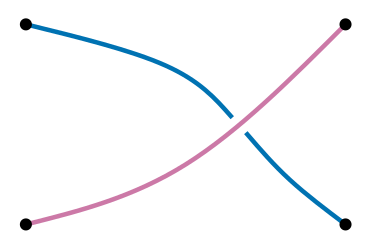
\includegraphics[width=.9\linewidth]{Inkscape Files/2braid2.png}
		\end{subfigure}
		\caption{These 2-braids are not equivalent}
		\label{unequal2braids}
	\end{figure}
\end{example}

The braid equivalence we have defined turns out to be an equivalence relation
(Def. \ref{equivrel}). But arguably this is what we would expect: after all, we
\emph{want} to partition big collections of braids into subsets of braids that are
equivalent. As desired, the equivalence class of any braid ends up being the
set of all braids equivalent to it.

From now on, when we say braid, we will actually
be referring to the whole class of braids we have deemed equivalent. When we
say, for example, that \(\beta\) is a braid, remember \(\beta\) is a
representative of some class of equivalent braids.


\begin{definition}\label{braidgroup}
	\begin{informal}
	   Now that we have put our intuition of equivalent braids into mathematics,
		we can see this structure is truly a very natural one, despite the
		complicated formalisms. We can now define a product on the set of braids
		that is nice enough to form a group structure. 

		The product of braids \(\beta\) and \(\beta'\) with the same number of
		strands is simply	connecting \(\beta'\) to the end of \(\beta\).
		Technically, braids must be parameterized by the interval \([0, 1]\), so
		the new braid will have	to be reparameterized to travel the two braids
		twice as fast.

		Therefore, we can now form a \emph{braid group}, whose elements are
		equivalence classes of braids with the some fixed number of strands, and
		where the multiplication is concatenating the braids.
	\end{informal}

	\begin{formal}
	   We define the \textbf{braid group on \(n\) strands} \(B_n\) to be the set of
		equivalence classes of braids where the product of any two braids
		\(\{f_i : 1\le i\le n\}\), \(\{g_i : 1\le i\le n\}\) is \(\{h_i: 1\le i\le
		n\}\) where for all \(1\le i\le n\), 
		\[
			h_i(t) = f_i(t)\ast g_i(t) = 
			\begin{cases}
				f_i(2t)&\text{if }0\le t\le \frac{1}{2},\\
				g_{\overline{f}(i)}(2t-1)&\text{if }\frac{1}{2}\le t\le 1.
			\end{cases}
		\] 
	\end{formal}
\end{definition}
Indeed, we can verify the braid product \(\ast\) is well-defined. That is,
if we have \(\beta_i\) and \(\beta_i'\) are equivalent for \(i = 1, 2\), then
\(\beta_1\ast\beta_2\) and \(\beta_1'\ast\beta_2'\) are equivalent: there is no
ambiguity in choice of representatives. Moreover, we can verify \(\ast\) is
associative, that the braid given by \(f_i(t) = p_i\) for all \(1\le i\le n\)
gives an identity element in \(B_n\), and that the mirror image of every braid
is its inverse.

Every one of these properties can be seen by just drawing pictures. In the
process, we would also realize that the notion of equivalence was essential
here.
\begin{example}\label{idinv}
   In Figure \ref{productbraids}, we see two examples of braid products.
	Observe in (a) that when we take the product of a braid with the identity,
	we can pull the braid back to the 
	\begin{figure}[h!]
		\begin{subfigure}{.575\textwidth}
			\centering
			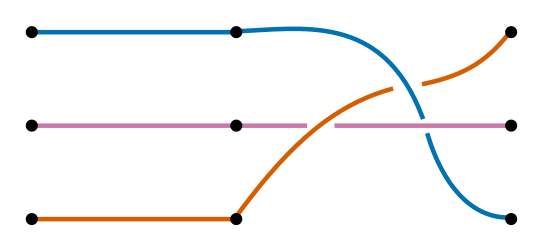
\includegraphics[width=.9\linewidth]{Inkscape Files/productbraid2.png}
		\end{subfigure}%
		\begin{subfigure}{.425\textwidth}
			\centering
			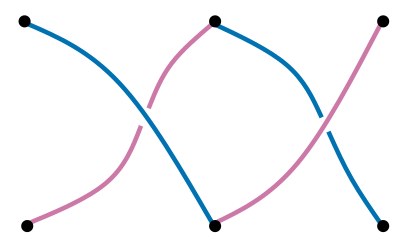
\includegraphics[width=.9\linewidth]{Inkscape Files/braidsum.png}
		\end{subfigure}
		\caption{(a): On the left is the product of the 2 braids of Figure
		\ref{3-braids}, denote it \(e\ast\sigma\). Note that \(e\ast\sigma =
		\sigma = \sigma\ast e\), since we can always pull the product strand back to
		\(\sigma\). (b): On the
		right is the product of the braids of Figure \ref{unequal2braids}. Note
		their product can be deformed to the identity, so they are inverses.}
		\label{productbraids}
	\end{figure}
\end{example}
None of these identities or inverses of the last example (Example \ref{idinv})
would have worked without the liberty to
pull strands around. Associativity similarly relies on this as well, since
different parenthesis placement results in the component braids taking up
different shares of space in their product. If the author's shady reasoning is
to be believed, then we well and truly have a group!

\begin{example} 
	Figure \ref{more-braid-mult} showcases more braid multiplication in \(B_2\),
	just for fun!
	\begin{figure}[h!]
		\begin{subfigure}{.5\textwidth}
			\centering
			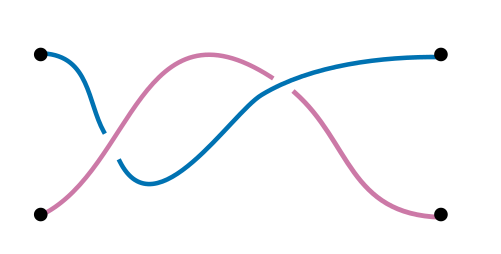
\includegraphics[width=.9\linewidth]{Inkscape Files/sigma1.png}
			\caption{\(\sigma_1\)}
		\end{subfigure}%
		\begin{subfigure}{.5\textwidth}
			\centering
			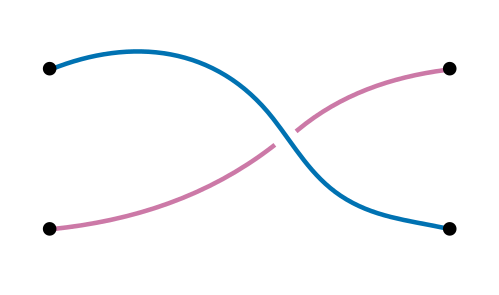
\includegraphics[width=.9\linewidth]{Inkscape Files/sigma2.png}
			\caption{\(\sigma_2\)}
		\end{subfigure}%
		\\  
		\begin{subfigure}{.5\textwidth}
			\centering
			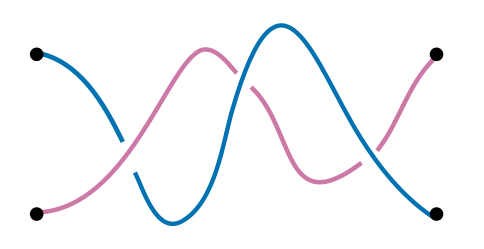
\includegraphics[width=.9\linewidth]{Inkscape Files/sigma1sigma2.png}
			\caption{\(\sigma_1\ast\sigma_2 = \sigma_2^{-1}\) by pulling up the pink
			through\\ and pushing down the blue crest.}
		\end{subfigure}%
		\begin{subfigure}{.5\textwidth}	  
			\centering
			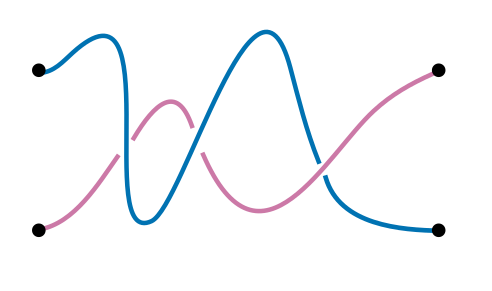
\includegraphics[width=.9\linewidth]{Inkscape Files/sigma2sigma1.png}
			\caption{\(\sigma_2\ast\sigma_1 = \sigma_2^{-1}\) by pulling up the blue
			through and pushing down the pink crest.}
		\end{subfigure}%
		\caption{Braids in \(B_2\).}
		\label{more-braid-mult}
	\end{figure}
\end{example}

\begin{example}
   The braid group on \(1\) strand has just one element: the braid
	given by just a single straight line. Therefore, \(B_1\cong\{e\}\) where
	\(\{e\}\) is the trivial group (Def. \ref{trivial-group}).

	One can show the braid group on \(2\) strands is isomorphic to
	\((\mathbb{Z}, +)\).
\end{example}

\begin{example}
   One thing we can observe about \(B_n\) is that none of the braid groups
	for \(n > 2\) are abelian.	The strategy is simple: each braid \(\{f_i: 1\le
	i\le n\}\) has a corresponding permutation \(\overline{f}\in S_n\). Then
	given two braids \(\beta, \beta'\in B_n\) with permutations \(\sigma,
	\sigma'\in S_n\), the permutation of \(\beta\ast\beta'\) must be
	\(\sigma'\circ\sigma\). Likewise, \(\beta'\ast\beta\) must have permutation
	\(\sigma\circ\sigma'\).

	However, \(S_n\) is not abelian for \(n > 2\), so \(B_n\) cannot be abelian
	for \(n>2\) as well. One neat way to see this is to recall the Dihedral
	group \(D_3\) from Example \ref{D3}, where from Figure \ref{D3operations},
	\(F_3\circ R \ne R\circ F_3\). But from the discussion in Definiton
	\ref{homiso}, elements of \(D_3\) can be regarded as elements in \(S_3\).
	Thus, take any braids \(\beta, \beta'\in B_n\) that permute the first three
	points \(p_1, p_2, p_3\) via \(R\) and \(F_3\) respectively (we can prove
	these exist simply by drawing an example). Then it cannot possibly be that
	\(\beta\ast\beta' = \beta'\ast\beta\).
\end{example}

\section{Mapping Class Groups}\label{mapping-class-groups}
Now we have finally defined braid groups, but how do they relate to the
symmetries of a disk? Like how we considered braids to be same up to
``nudging,'' we now want to do the same for functions. Doing so will be a much
more straightforward applications of the definitions from Section
\ref{homotopy-section}.

\begin{definition}
   Let \(U\subset\mathbb{R}^n\) be an arbitrary subset of \(\mathbb{R}^n\),
	\(V\subset U\) an arbitrary subset of \(U\). We define 
	\[
		\Homeo(U, V) = \{f: U\to U \mid f~\text{a homeomorphism such
		that}~f(v)=v~\text{for all}~v\in V\}.
	\] 
	In other words, \(\Homeo(U, V)\) is the set of all homeomorphisms of
	\(U\) to itself that fix \(V\) pointwise. Under composition, \(\Homeo(U,
	V)\) is a group.
\end{definition}
\begin{remark}
   As with homotopies, this definition extends to arbitrary topological spaces.
\end{remark}

We will now use this group to define a relation.
\begin{definition}\label{isotopic-in-homeo}
	Let \(f, g\in \Homeo(U, V)\) be arbitary. We say \(f\) and \(g\) are
	\textbf{isotopic in \(\Homeo(U, V)\)} if there is an isotopy 
	\[
		F: U\times [0, 1]\to U
	\]
	from \(f\) to \(g\) such that for all \(t\in [0, 1]\),
	\(F_t\in\Homeo(U, V)\).
\end{definition}
Note that the use of isotopy rather than homotopy in the last definition (Def.
\ref{isotopic-in-homeo}) is unnecessary since the only allowed \(F_t\) are
homeomorphisms anyway. Nonetheless, it is standard to say isotopy.

Isotopy in \(\Homeo(U, V)\) defines an equivalence relation, which
gives a partition of the set \(\Homeo(U, V)\) into subsets of functions that are
isotopic in \(\Homeo(U, V)\). Like with braids, we would like to regard
isotopic functions as equivalent and work with the equivalence classes. But do
the resulting equivalence classes form another group?

The answer lies in the subset 
\[
	\Homeo_0(U, V) = \{f\in\Homeo(U, V) : f~\text{is isotopic
	to}~\id~\text{in}~\Homeo(U, V)\}.
\]

\begin{proposition}
  \(\Homeo_0(U, V)\) is a normal subgroup of \(\Homeo(U, V)\).
\end{proposition}
\begin{proof}
	First, we will show \(\Homeo_0(U, V)\) is a subgroup of \(\Homeo(U, V)\).
	Suppose \(f, g\in\Homeo_0(U, V)\). Then there exist isotopies \(F, G:
	U\times [0, 1]\to U\) from \(f\) and \(g\) to the identity such that for all
	\(t\in[0, 1]\), \(F_t, G_t\) are
	homeomorphisms that fix \(V\) pointwise. It follows that the function
	defined by 
	\begin{align*}
		H: U\times [0, 1]\to U,\\
		H(x, t) = F(G(x, t), t)
	\end{align*}
	is a homotopy from \(f\circ g\) to \(\id\) such that for all
	\(t\in [0, 1]\), \(v\in V\), \(H_t(v) = v\).
	Moreover, the function defined by 
	\begin{align*}
		J: U\times [0, 1]\to U,\\
		J(x, t) = F_t^{-1}(x)
	\end{align*}
	is a homotopy from \(f^{-1}\) to \(\id\) that also fixes
	\(V\) pointwise. It follows that \(\Homeo_0(U, V)\) is a subgroup.

	Next, we will show \(\Homeo_0(U, V)\le\Homeo(U, V)\) is normal. Let
	\(f\in\Homeo_0(U, V)\), \(g\in\Homeo(U, V)\) be arbitrary. Then let \(F:
	U\times [0, 1]\to U\) be an isotopy of \(f\) to the identity in \(\Homeo(U,
	V)\). It follows that the function defined by 
	\begin{align*}
		H: U\times [0, 1]\to U,\\
		\quad H(x, t) = (g\circ F)(g^{-1}(x), t)
	\end{align*} 
	is a homotopy from \(g\circ f\circ g^{-1}\) to \(\id\) in
	\(\Homeo(U, V)\). Thus, \(g\circ f\circ g^{-1}\in\Homeo_0(U, V)\), so
	\(\Homeo_0(U, V)\trianglelefteq\Homeo(U, V)\).
\end{proof}

We will now see why the normality of \(\Homeo_0(U, V)\) is essential to
creating our desired group.
\begin{proposition}
   Let \(\sim\) be the relation on \(\Homeo(U, V)\) where for all \(f,
	g\in\Homeo(U,V)\), \(f\sim g\) if and only if \(f\) and \(g\) are isotopic
	in \(\Homeo(U, V)\). Then the equivalence classes of \(\sim\) are exactly
	the cosets \(\Homeo_0(U, V)\) in \(\Homeo(U, V)\).
\end{proposition}
\begin{proof}
   It is sufficient to show that given any \(f\in\Homeo(U, V)\), 
	\[
		[f]_\sim = f\Homeo_0(U, V).
	\] 
	Suppose \(g\in [f]_\sim\). Then \(g\) is isotopic to \(f\) in
	\(\Homeo(U, V)\). Let \(F: U\times [0, 1]\to U\) be an isotopy from \(g\) to
	\(f\) in \(\Homeo(U, V)\). Then
	observe the function 
	\begin{align*}
		H: U\times [0, 1]\to U,\\
		H(x, t) = (f^{-1}\circ F)(x, t)
	\end{align*} 
	is an isotopy from \(f^{-1}\circ g\) to \(\id\) in \(\Homeo(U,
	V)\).
	This means that \(f^{-1}\circ g\in\Homeo_0(U, V)\). But then 
	\[
		g = f\circ (f^{-1}\circ g) \in f\Homeo_0(U, V).
	\] 
	Conversely, suppose \(g\in f\Homeo_0(U, V)\). Then \(g = f\circ h\)
	where \(h\in\Homeo_0(U, V)\). Let \(F: U\times [0, 1]\to U\) be an isotopy
	from \(h\) to \(\id\) in \(\Homeo_0(U, V)\). It follows that the function
	\begin{align*}
		H: U\times [0, 1]\to U,\\
		H(x, t) = (f\circ F)(x, t)
	\end{align*}
	is an isotopy from \(f\circ h = g\) to \(f\) in \(\Homeo_0(U,
	V)\). Thus, \(g\in[f]_\sim\). We conclude 
	\[
		[f]_\sim = f\Homeo_0(U, V).
	\] 
	Therefore, the equivalence classes \([f]_\sim\) are the same as the
	cosets of \(\Homeo_0(U, V)\).
\end{proof}

This finally allows us to define our desired group of equivalence classes.
\begin{definition}[Mapping class groups]\label{mcg}
	\begin{informal}
		Recall how in the last section (Section \ref{introduction-to-braids}), we
		grouped together all braids that were reasonably similar and considered
		them as one object. When we formed the braid groups, we operated on these
		classes of objects, and in fact this was necessary to reveal the group
		structure.

		In this case, the situation is not quite as difficult. \(\Homeo(U, V)\) is
		already a group. When our functions in 
		\(\Homeo(U, V)\) can be reasonably nudged to be the same, we want to
		regard them as equivalent and operate on
		those equivalence classes themselves.

		In short, we want to turn the set of equivalence classes \([f]_\sim\)
		into a group. In this case, normal subgroups come to our rescue. The
		desired equivalence classes are, as luck would have it, precisely the
		cosets of a normal subgroup. The resulting quotient group has elements
		\([f]_\sim\) and inherits our desired group structure. We call this the
		\emph{mapping class group} \(MCG(U, V)\) and call the equivalence classes
		\([f]_\sim\) \emph{mapping classes}.
	\end{informal}

	\begin{formal}
	   The \textbf{mapping class group} of \(U\) with respect to \(V\) is the
		quotient group 
		\[
	      MCG(U, V) = \Homeo(U, V) / \Homeo_0(U, V).
	   \]
	\end{formal}
\end{definition}

We will denote mapping classes simply as \([f]\), dropping the \(\sim\). Very
often, even the brackets are dropped, but we will avoid doing so in this paper.

We will work out a relevant example that will soon become very important: the
mapping class group of the disk
\(D^2\) with respect to its boundary circle \(S^1\subset D^2\).

\begin{lemma}[Alexander trick {\cite[p.~47]{primer}}]\label{alexander-trick}
   The group \(MCG(D^2, S^1)\) is trivial.
\end{lemma}
\begin{proof}
	Let \([f]\in MCG(D^2, S^1)\) be a mapping class. Then function \(F:
	D^2\times [0, 1]\to D^2\) defined by
	\[
	   F(x, t) = 
		\begin{cases}
			(1-t)f\left(\frac{x}{1-t}\right) &\text{if } 0\le \abs{x} < 1-t,\\
			x &\text{if } 1-t\le\abs{x}\le 1,
	   \end{cases}
	\] 
	for all \(t\in[0, 1]\) is an isotopy of \(f\) to \(\id\) in \(\Homeo(D^2,
	S^1)\).
\end{proof}
The idea of the Alexander trick is that for every \(t\in[0, 1]\), we apply
\(f\) on a smaller disk of radius \(1-t\). The factor of \(1-t\) inside of
\(f\) allows us to map every point of \(D^2\) for each \(t\), while the factor
of \(1-t\) outside shrinks the image to another disk of radius \(1-t\). While
we shrink \(f\) to a homeomorphism of smaller and smaller disks, we switch out
the remaining space with the identity map. See Figure \ref{Alex-trick-pic} for
a visual.

\begin{figure}
   \centering
	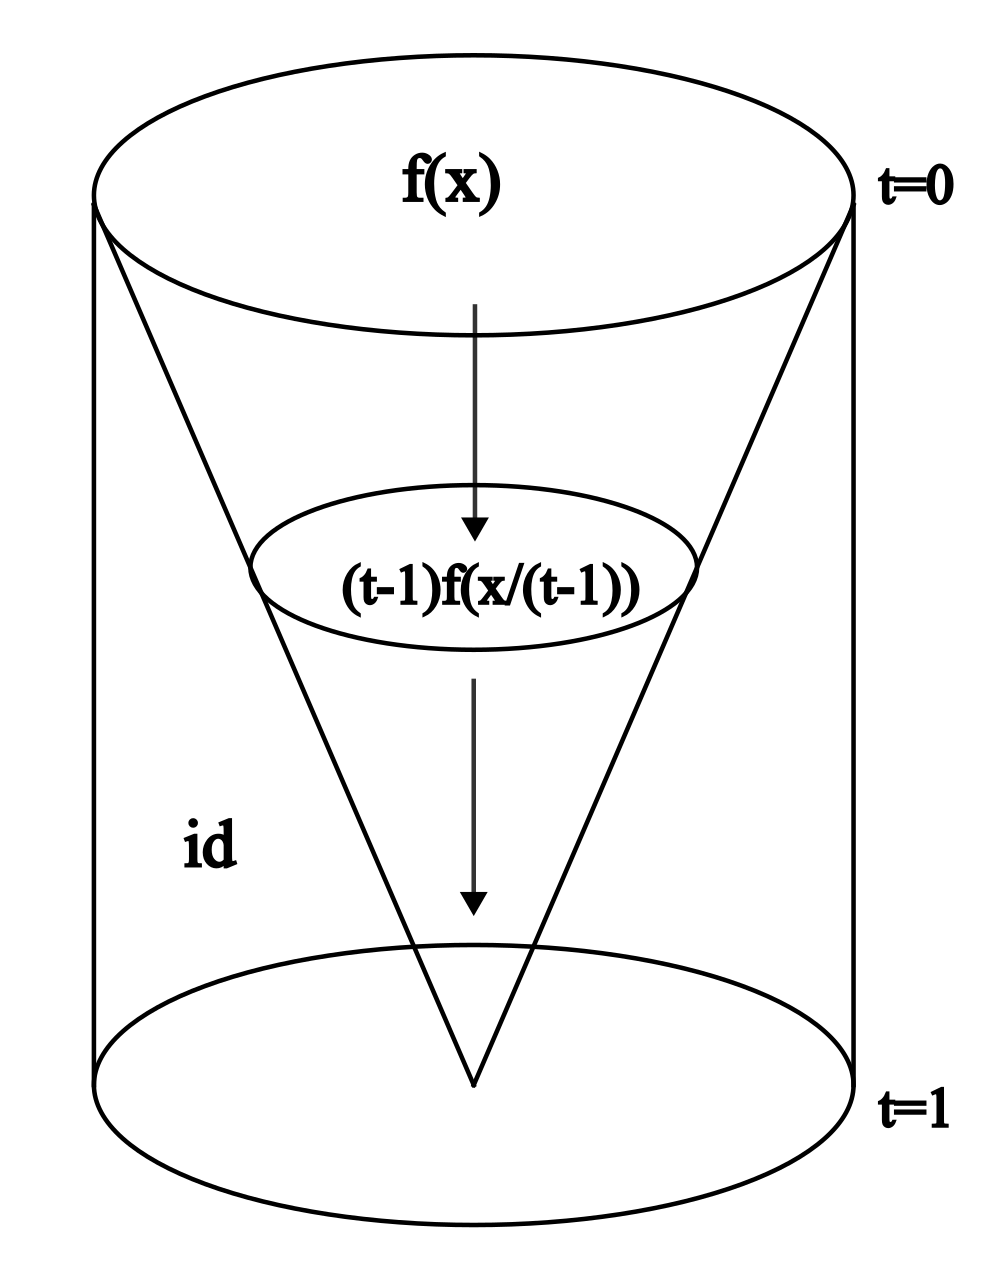
\includegraphics[width = .35\textwidth]{Inkscape Files/alexander-trick.png}
	\caption{A standard visual of the Alexander trick by taking the function
		\((F(x, t),	t)\) where \(F\) is the isotopy. In other words, we are
		taking what \(F(x, t)\) is at each time and moving that slightly out of
		the way of what it was before. No information is lost and we get a nice
		visualization.}
	\label{Alex-trick-pic}
\end{figure}

However, the key point is this: every homeomorphism of the disk, so long as it
fixes the boundary \(S^1\), is homotopic to the identity. What this means is,
like how we could interpret the function \(r\) in Example \ref{first-squishing} as
squishing the cylinder, we can think of every boundary-fixing homeomorphism of
the disk as some continuously pushing the points of the disk around. The
pushing here is formally in accordance with the isotopy \(F(x, 1-t)\) from
\(\id\) to \(f\), where \(F\) and \(f\) are defined as in Lemma
\ref{alexander-trick}.

Intuitively, this makes such homeomorphisms of a disk rather intuitive: it is
as if the disk were made of soft clay, and we are kneading it around while
ensuring the whole disk remains covered, and without moving the boundary or
breaking it.

This is not true in general for continuous functions or homeomorphisms. For
example, even the homeomorphism \(f: D^2\to D^2\) given by \(f(x) = -x\) cannot
be interepreted this way.

\begin{remark}
   For those who are interested, there is a lot to learn about mapping class
	groups. In particular, a lot of
	work has been done on the mapping class groups of surfaces, where for an
	orientable surface \(S\), we focus on 
	\[
	   MCG(S) = \Homeo^+(S, \partial S) / \Homeo_0(S, \partial S),
	\] 
	the mapping classes of orientation-preserving homeomorphisms. For
	example, we know that for every compact orientable surface, possibly with
	fintely many marked points that must be permuted, \(MCG(S)\) is
	finitely presented {\cite[p.~137]{primer}}, and we can write a presentation
	down. The same is true for compact non-orientable surfaces with
	finitely many marked points {\cite{korkmaz2002}}.

	For orientable surfaces, \cite{primer} is great (I think it's amazing!).
	For non-orientable surfaces, try
	\cite{paris2014}.
\end{remark}

\section{Punctured Disk and Braids}\label{punctured-disk-and-braids}
The group \(MCG(D^2, S^1)\) was the final piece we needed to formally connect
braids to disks.

\begin{theorem}[{\cite[p.~243]{primer}}]
	Let \(D_n\) denote \(D^2\setminus\{p_1, \ldots, p_n\}\). Assume none of the
	points \(p_i\) are on the boundary circle of \(D^2\). Then 
	\[
	   B_n\cong MCG(D_n, S^1).
	\]
\end{theorem}
This is not very elementary to prove, but the intuition is much easier. First,
we must state the following characterization of homeomorphisms \(D_n\to D_n\).
\begin{proposition}\label{puncture-markedpoints}
	Fix \(n\) points \(p_1,\ldots, p_n\in D^2\) not on the boundary. Let
	\(\Homeo_p(D^2, S^1)\) denote the subgroup of \(\Homeo(D^2, S^1)\) that
	permutes the \(p_i\)'s. In other words, for all \(f\in\Homeo_p(D^2, S^1)\),
	there exists \(\sigma\in S_n\) such that \(f(p_i) = p_{\sigma(i)}\) for all
	\(1\le i\le n\). Then \(\Homeo(D_n, S^1)\cong \Homeo_p(D^2, S^1)\).
\end{proposition}
\begin{proof}
	\begin{informal}
	   The proof of this is a bit technical, but the idea is this. Whenever we
		have a homeomorphism of the punctured disk \(D_n\), we can actually
		``fill in'' the punctures and send them to each other. For any \(f:
		D_n\to D_n\) a homeomorphism, \(f\) being a homeomorphisms ensures each
		of these punctures has one and only one other puncture they can go to. We
		find this by checking all the points around each puncture. By continuity,
		they must all be sent to an area roughly around another puncture. This
		allows us to extend functions of punctured disks to functions of
		the whole disk that simply permute the \(p_i\)'s around.

		This corresondence goes both ways. Given any homeomorphism that permutes
		the \(p_i\)'s, we can define a new homeomorphism \(D_n\to D_n\) just by
		restricting the domain to \(D_n\).

		The proof is on the technical side. A rigorous understanding of it is not
		required.
	\end{informal}
	\begin{formal}
	   Let \(f\in\Homeo(D_n, S^1)\), and pick mutually disjoint punctured
		neighborhoods \(U_i\) for each point \(p_i\). We will define
		\(\overline{f}\in S_n\) as follows. Since \(f\) is a
		homeomorphism, the image of
		each \(U_i\) must be another punctured neighborhood of some \(p_j\), \(1\le
		j\le n\). Let \(\overline{f}(i) = j\). Observe that \(\overline{f}\) is
		indeed a bijection. If \(i\ne j\), then the assumption \(U_i\cap U_j =
		\varnothing\) implies \(\overline{f}(U_i)\cap \overline{f}(U_j) =
		\varnothing\) because \(f\) is a homeomorphism. But all punctured
		neighborhoods of the same puncture must intersect. Thus,
		\(\overline{f}(i)\ne \overline{f}(j)\). It follows \(\overline{f}\) is
		injective, hence bijective.

		Then defining \(\widetilde{f}: D^2\to D^2\) by 
		\[
			\widetilde{f}(x) = 
			\begin{cases}
				f(x) &\text{if }x\in D_n\\
				p_{\overline{f}(i)} &\text{if }x = p_i
			\end{cases},
		\] 
		we have a homeomorphism \(\widetilde{f}\in\Homeo_p(D^2, S^1)\). This
		gives us a group homomorphism 
		\begin{align*}
			\Phi: \Homeo(D_n, S^1)&\to \Homeo_p(D^2, S^1),\\
			\Phi(f) &= \widetilde{f}.
		\end{align*}

		We can define another homomorphism 
		\begin{align*}
			\Psi:\Homeo_p(D^2, S^1)&\to\Homeo(D_n, S^1)\\
			\Psi(f) &= f|_{D_n}
		\end{align*}
		via restricting to \(D_n\). \(\Phi\) and \(\Psi\) are inverses,
		so we conclude 
		\[
			\Homeo(D_n, S^1)\cong\Homeo_p(D^2, S^1).
		\] 
	\end{formal}
\end{proof}

Therefore, whenever we consider a homeomorphism \(D_n\to D_n\), we may just as
well consider a homeomorphism \(D^2\to D^2\) that permutes the \(p_i\)'s. This
interpretation is quite useful --- recall the discussion after the Alexander
trick (Lemma \ref{alexander-trick}). Any homeomorphism \(D^2\to D^2\) that
fixes the boundary can be obtained by an isotopy in \(\Homeo(D^2, S^1)\) from the
identity.

This means that for any \(f\in\Homeo(D_n, S^1)\), we can intuitively think of
\(f\) as corresonding to some ``kneading'' of \(D^2\). To get \(f\), we
continuously move the
points of \(D^2\) around, gradually moving each point \(x\in D^2\) to where the
point \(f(x)\) used to be. At the end, remove the \(p_i\)'s. Since we're
thinking of deforming from the identity, this isotopy is the one from the
Alexander trick, but backwards: 
\[
   F(x, t) = 
	\begin{cases}
		xf\left(\frac{x}{t}\right) &\text{if }0\le \abs{x}\le t,\\
		x &\text{if }t\le\abs{x}\le 1.
   \end{cases}
\]
Really all we are doing is reversing where \(t=0\) and \(t=1\) are on Figure
\ref{Alex-trick-pic}.

But in this process, pay special attention to how
each point \(p_i\) traces out a
path on \(D^2\) to some \(p_{\overline{f}(i)}\) as time moves from \(t=0\) to
\(t=1\). There is the connection! For each \(p_i\), we are getting a path 
\[
	\gamma_i: [0, 1]\to D^2
\] 
defined by how the point \(p_i\) moves to \(p_{\overline{f}(i)}\). We will
now make one modification to the \(\gamma_i\) by defining 
\begin{align*}
	f_i: [0, 1]&\to D^2\times [0, 1],\\
	f_i(t) &= (\gamma_i(t), t).
\end{align*} 
In effect, the \(f_i\)'s ``raise'' the paths outside of \(D^2\),
having them move forward as time passes. This is illustrated in Figure
\ref{alex-braid}.

\begin{figure}
   \centering
	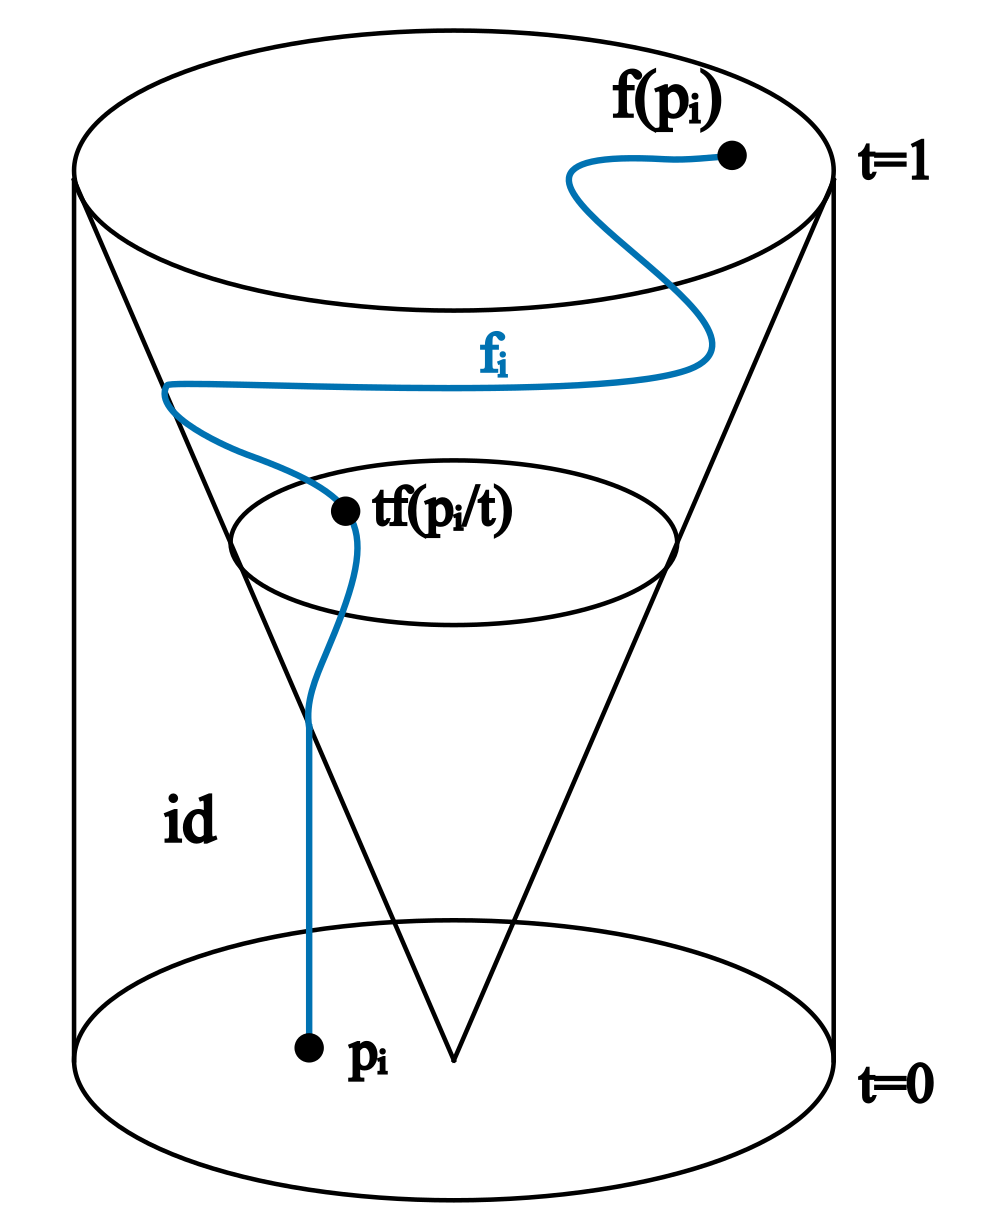
\includegraphics[width = 0.4\textwidth]{Inkscape Files/alexander-braid.png}
	\caption{Observe how the Alexander lemma gives rise to the strands of a
	braid.}
	\label{alex-braid}
\end{figure}

Observe that by definition, we have:
\begin{enumerate}[label=(\roman*)]
	\item the images \(f_i[0, 1]\) are disjoint. This is because if for any time
	\(t\), \(f_i(t) = f_j(t)\) for some \(i\ne j\), then this implies that
	\(p_i\) and \(p_j\) were moved to the same location in the ``kneading''
	process. As we have covered, this is not allowed. 

	Physically, this means the paths we have defined never intersect each other.
	\item \(f_i(0) = (\gamma_i(0), 0) = (p_i, 0)\).
	\item \(f_i(1) = (\gamma_i(1), 1) = (p_{\overline{f}(i)}, 1)\).
	\item For any \(t\in[0, 1]\), \(f_i(t) = (\gamma_i(t), t)\in
	D^2\times\{t\}\).
\end{enumerate}
But recall from Definition \ref{braids} that these conditions are precisely
what defines a braid. Thus, from an arbitrary homeomorphism \(f: D_n\to D_n\),
we have obtained \(\{f_i: 1\le i\le n\}\), a braid on \(n\) strands! Let's call
\(\{f_i: 1\le i\le n\} = \beta_f\). But does this association still make sense
for mapping classes?

Let's at least verify first that isotopic functions in \(\Homeo(D_n, S^1)\)
give equivalent braids.

\begin{proposition}\label{well-defined-braid}
   The function 
	\[
      \Phi: MCG(D_n, S^1)\to B_n
   \]
	defined by
	\[
		\Phi([f]) = \{f_i: 1\le i\le n\} = \beta_f
   \] 
	as in the preceding discussion is well-defined.
\end{proposition}
\begin{proof}
	\begin{informal}
		We wish to show that \(\Phi\) makes sense. Of course, given an arbitrary
		homeomorphism in \(\Homeo(D_n, S^1)\), it makes sense by our discussion
		that we just get the braid \(\beta_f\). But for a quotient group like
		\(MCG(D_n, S^1)\), if we take an arbitrary mapping class \([f]\), do we
		get \(\beta_f\) regardless of what representative we choose. It is not
		immediately clear that if \(g\in [f]\), \(\beta_g\) is equivalent to
		\(\beta_f\).

		The way we do it here is by working explicitly with the braid formulas
		for \(f\) and \(g\) given by the Alexander trick, then extending the
		isotopy \(H\) from \(f\) to \(g\) to the entire braid. Visually, we are
		moving the
		whole braid from \(f\) to \(g\) in accordance with \(H\). A bit more
		technical work is done to make this an ambient isotopy.

	   Ostensibly, this is the first step of a proof that \(MCG(D_n, S^1)\cong
		B_n\). Using this strategy, we would want to show that \(\Phi\) is also a
		homomorphism, and in fact bijective (technically, \(\Phi\) is not a
		homomorphism in its current state, but we address this later). However,
		this is not how this
		theorem is conventionally proven. The proof is not easy, and we
		use much more powerful tools to tackle it. The following
		argument is included just to make the theorem seem more convincing using
		only elementary arguments. It may also demonstrate why
		continuing in this manner is not very sustainable.
	\end{informal}

	\begin{formal}
		Suppose \(f\sim g\) in \(\Homeo(D_n, S^1)\). Then let \(F, G:
		\mathbb{D}\to D^2\) be the isotopies from \(\id\) to \(F\) and \(G\)
		respectively given by the Alexander trick.
		We use these to define \(\widetilde{F}, \widetilde{G}: \mathbb{D}\to
		\mathbb{D}\),
		\begin{align*}
			\widetilde{F}(x, s) &= (F(x, s), s),\\
			\widetilde{G}(x, s) &= (G(x, s), s).
		\end{align*}

		Since \(f\sim g\), let \(H: \mathbb{D}\to\mathbb{D}\) be an isotopy from
		\(\id\) to \(g\circ f^{-1}\) (given by filling in the missing points
		of the corresponding isotopy in \(\Homeo(D_n, S^1)\)). Then \(h:
		\mathbb{D}\times[0, 1]\to\mathbb{D}\) defined by 
		\[
			h((x, s), t) = 
			\begin{cases}
				\left(sH\left(\frac{x}{s}, t\right), s\right) &\text{if}
				0\le\abs{x}\le s,\\
				(x, s) & \text{if }s\le\abs{x}\le 1.
			\end{cases}
		\] 
		satisfies 
		\begin{enumerate}[label=(\roman*)]
			\item for all \(t\in[0, 1]\), \(h_t: \mathbb{D}\to\mathbb{D}\) is a
			homeomorphism,
			\item for all \(t\in[0, 1]\), \(h_t\) fixes the boundary of
			\(\mathbb{D}\),
			\item \(h_0(x, s) = (x, s)\) is the identity and 
			\begin{align*}
				h_1(f_i(s)) = h_1(F(x, s), s) &= 
				\begin{cases}
					\left(s(g\circ f^{-1})\left(\frac{F(p_i, s)}{s}\right),
					s\right)&\text{if}0\le\abs{F(p_i, s)}\le s,\\
					(F(p_i, s), s) &\text{if }s\le\abs{F(p_i, s)}\le 1
				\end{cases} \\
				&= 
				\begin{cases}
					\left(s(g\circ f^{-1})\left(\frac{sf\left(\frac{p_i}{s}\right)}{s}
					\right), s\right) &\text{if }0\le \abs{p_i}\le s,\\
					(p_i, s)&\text{if } s\le \abs{p_i}\le 1
				\end{cases}\\
				&= 
				\begin{cases}
					\left(sg\left(\frac{p_i}{s}\right), s\right) &\text{if }0\le
					\abs{p_i}\le s,\\
					(p_i, s) &\text{if }s\le\abs{p_i}\le 1
				\end{cases}\\
				&=\widetilde{G}(p_i, s) = g_i(s).
			\end{align*}
		\end{enumerate}
		It follows that \(h\) is an ambient isotopy taking \(\beta_f\) to
		\(\beta_g\), so \(\beta_f\) and \(\beta_g\) are the same braid. Thus,
		\(\Phi\) is independent of our choice of mapping class representative and
		therefore well-defined.
	\end{formal}
\end{proof}

In the discussion preceding the proof of Proposition \ref{well-defined-braid},
we briefly mentioned \(\Phi\) is not technically a homomorphism in its current
state. This is because it's backwards: \(\Phi([f]\circ[g]) =
\beta_g\ast\beta_f\). The reason is that \(f\circ g\) is the function that
applies \(g\) first, then \(f\); meanwhile \(\beta_f\ast\beta_g\) is first the
braid given by \(f\), then the braid given by \(g\).

The fix for this is easy. We just redefine composition in \(MCG\) to go
backwards. We will say \((f\circ g)(x) = g(f(x))\). This is not too
unreasonable: if \(\beta\ast\beta'\) is first \(\beta\), then \(\beta'\), then
why should \(f\circ g\) be \(g\) first, then \(f\)? In some texts, this is
the convention, and it ultimately makes no difference to the group structure
(they are isomorphic). We will make this adjustment moving forward (I did not
introduce it this way because it confuses me a lot).

The proof \(\Phi\) is a homomorphism, and indeed an isomorphism, is much more
involved. We will omit it in lieu of a more intuitive discussion.

\begin{comment}
   I am not actually aware if there is an elementary proof in this style.
	Probably there is a way to at least show \(\Phi\) is a homomorphism, but I
	have not found or constructed an elementary argument for it using just
	ambient isotopy. If anyone has or knows of one, I would love to know it!
\end{comment}

Ultimately, what does this isomorphism tell us about the relationship between
braids and homeomorphisms of the punctured disk? 

\begin{enumerate}[label=(\roman*)]
	\item First, the very fact \(\Phi\) is a homomorphism tells us that if we
	deform the disk in accordance to \(f\), then in accordance to \(g\), that
	very process is no different (up to isotopy by homeomorphisms) to deforming
	the disk in accordance to \(f\circ g\).

	\item Second, that \(\Phi\) is a bijective tells us that every braid arises
	from a mapping class of homeomorphisms in \(\Homeo(D_n, S^1)\). Likewise,
	every mapping class of homeomorphisms in \(\Homeo(D_n, S^1)\) uniquely gives
	a braid --- any other mapping class will give a different braid.

	\item Third, from the correspondence of mapping classes and braids, we see
	that kneading around a
	homeomorphism in \(\Homeo(D_n, S^1)\) is essentially no different from
	nudging around a braid on \(n\) strands.
\end{enumerate}

This brings us to our final point: by endowing group structures to our objects
--- homeomorphisms and braids --- we are able to speak precisely about the
correspondence of structures between homeomorphisms and braids. Braids and
mapping classes in \(MCG(D_n, S^1)\) correspond one-to-one, and the natural
operations on each correspond perfectly as well. Up to multiplying, these are
exactly the same.

Besides just being interesting, this correspondence is quite useful for talking
about mapping classes in general. For example, while homeomorphisms can be
rather difficult to write down explcitly, in the case of the disk, we can
simply specify a braid rather than write down an explicit formula. Writing down
and composing functions can all be substituted by drawing braids. Or we
can tell if two functions are the same by examining their braids. and when we
compose functions, we need only multiply their braids.

This is not limited to the disk. ``Surfaces,'' such as the sphere, torus, klein
bottle, etc. all contain disks. If a torus has some punctures in it, we can cut
out a disk, apply braids, then glue that disk back to get a mapping class of
the torus (we call this a \emph{half dehn twist}). 

This means, remarkably, that braids do not just describe the mapping classes of
a punctured disk, but in fact of all shapes that have disks inside of them. All
because we realized braids can be multiplied.

\section{The proof?}
The main storyline of this paper is over, but probably there are readers
interested in the proof that \(MCG(D_n, S^1)\cong B_n\). 

The techniques are quite beyond the scope of this paper, but they are worth
learning. They are accessible after a typical first course in algebraic
topology.

The braid group on \(n\) strands is the same as the fundamental group of the
unordered configuration space \(C(D^2, n)\). Then we use the generalized
\emph{Birman exact sequence}, where for any orientable surface \(S\), \(S_n =
S\setminus\{p_1, \ldots, p_n\}\), there is an exact sequence 
\[
	1 \to \pi_1(C(S, n))\xrightarrow{\text{Push}} MCG(S_n, \partial
	S_n)\xrightarrow{\text{Forget}} MCG(S, \partial S)\to 1.
\]
Roughly, we define Push by taking \emph{Dehn twists} around the loops in
\(C(S, n)\), Forget is the natural map where we fill in the punctures, and the
exact sequence is obtained by the long exact sequence of homotopy groups of the
fiber bundle (the LES of a fiber bundle is covered in Chapter 4 of
{\cite{hatcherAT}}),
\[
   \Homeo^+(S_n, \partial S_n)\to \Homeo^+(S, \partial S) \to C(\itr (S), n).
\] 
Of course, since \(MCG(D^2, S^1)\) is trivial, we get 
\[
   B_n\cong \pi_1(C(D^2, n))\cong MCG(D^2, S^1).
\]
The full exposition is covered in detail in \cite{primer}.




\printbibliography 


\end{document}
